\documentclass[titlepage,a4paper,12pt]{report}
\usepackage{amssymb,amsfonts,amsmath}
\usepackage{fullpage}
\usepackage{graphicx}
%\usepackage[cc]{titlepic}
\usepackage{amsthm}
\newtheorem{definition}{Definition}[section]
\newtheorem{example}{Example}[section]
\newtheorem{theorem}{Theorem}[section]
\newtheorem{exercise}{Exercise}[section]
\newtheorem{corollary}{Corollary}[section]
\newtheorem{proposition}{Proposition}[section]
\pdfpagewidth 8.5in
\pdfpageheight 11in
\setlength\topmargin{-0.5in}
\setlength\headheight{0in}
\setlength\headsep{0in}
\setlength\textheight{9.5in}
\setlength\textwidth{7.0in}
\setlength\oddsidemargin{-0.5in}
\setlength\evensidemargin{1.0in}
\setlength\parindent{0.25in}
\setlength\parskip{0.25in}
%\begin{titlepage}
%\usepackage{titlepic}
%\titlepic{
\includegraphics[width=0.2\textwidth]{uz1.png}}
%
%\title{\textbf{HMTH111 Calculus 2}}
%\author{Nhawu. G\\
%		Department of Mathematics\\
%		University of Zimbabwe, ZIM}
%
%\end{titlepage}

\begin{document}
\begin{titlepage}
 
\begin{center}
 
 
% Upper part of the page

\includegraphics[width=0.15\textwidth]{uz1.png}\\[1cm]
 
\textsc{\LARGE University of Zimbabwe}\\[1.5cm]
 
\textsc{\Large HMTHCS111 CALCULUS 2}\\[0.5cm]
 
 
% Title

{ \huge \bfseries Calculus of Several Variables}\\[0.4cm]
 

 
% Author and supervisor
\begin{minipage}{0.4\textwidth}
\begin{center} \large
\emph{Author:}\\
G. \textsc{Nhawu}
\end{center}
\end{minipage}
\begin{minipage}{0.4\textwidth}
\begin{flushright} \large
\emph{Department:} \\
\textsc{Mathematics and Computational Sciences}
\end{flushright}
\end{minipage}

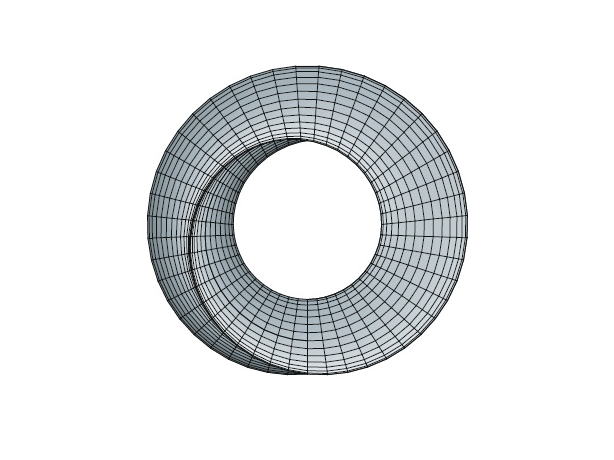
\includegraphics[width=0.7\textwidth]{umblictorus.png}\\[1cm]
 \vfill
 
 
% Bottom of the page
{\large \today}
 
\end{center}
 
\end{titlepage}
%\maketitle
\tableofcontents
\begin{abstract}
\begin{center}
	\small{\parbox{18cm}{
		\begin{raggedright}
		{\small
		\textit{Everybody is a genius. But if you judge a fish by its ability to climb a tree, it will live its whole life believing that it is stupid.}
 }
 
				\vspace{.5cm}\hfill{---Albert Einstein}
		\end{raggedright}
	}
} 
\end{center}
These notes are not intended as a textbook. It is hoped however that they will minimize the amount of note-taking activity which occupies so much of a student’s class time in most courses in Mathematics. Probably the most important aspect of the notes is the set of tutorials. You should develop the practice of attempting several of these problems every week. Many of the problems are quite difficult so please consult your
tutor/lecturer if you are not blessed with success initially. Do not acquire the habit of abandoning a problem if it does not yield to your first attempt; a defeatist
attitude is your greatest adversary. Solution of a problem, even with some assistance
from the teacher when necessary, is a fine boost to your morale. You will find that a strong effort expended on the earlier part of the courses will be rewarded by growing
self-confidence and easier success later.

\noindent The emphasis is on understanding concepts. I think that nearly everybody agrees that
this should be the primary goal of calculus instruction. In fact, the impetus for the current
calculus reform movement came from the Tulane Conference in 1986, which formulated
as their first recommendation:
\begin{center}
\textit{Focus on conceptual understanding}.
\end{center}

\noindent I have tried to implement this goal through the \textit{Rule of Three}: ``Topics should be presented
geometrically, numerically, and algebraically.'' Visualization, numerical and graphical experimentation,
and other approaches have changed how we teach conceptual reasoning in fundamental
ways. The Rule of Three has been expanded to become the \textit{Rule of Four} by
emphasizing the verbal, or descriptive, point of view as well.
\end{abstract}
\chapter{What is Calculus?}
\begin{center}
	\small{\parbox{18cm}{
		\begin{raggedright}
		{\small
		\textit{A great discovery solves a great problem but there is a grain of discovery in the
solution of any problem. Your problem may be modest; but if it challenges your
curiosity and brings into play your inventive faculties, and if you solve it by your
own means, you may experience the tension and enjoy the triumph of discovery.}
 }
 
				\vspace{.5cm}\hfill{---George Poyla}
		\end{raggedright}
	}
} 
\end{center}
To a Roman in the days of the empire, a ``calculus'' was a pebble used in counting and
gambling. Centuries later, ``calculare'' came to mean ``to calculate,'' ``to compute,'' ``to
figure out.'' For our purposes, calculus is elementary mathematics (algebra, geometry,
trigonometry) enhanced by the \textit{limit process}.

\noindent It is fitting to say something about the history of calculus. The origins can be traced
back to ancient Greece. The ancient Greeks raised many questions (often paradoxical)
about tangents, motion, area, the infinitely small, the infinitely large, ---questions that
today are clarified and answered by calculus. Here and there the Greeks themselves
provided answers (some very elegant), but mostly they provided only questions.

\noindent After the Greeks, progress was slow. Communication was limited, and each scholar
was obliged to start almost from scratch. Over the centuries, some ingenious solutions
to calculus-type problems were devised, but no general techniques were put forth.
Progress was impeded by the lack of a convenient notation. Algebra, founded in the
ninth century by Arab scholars, was not fully systematized until the sixteenth century.
Then, in the seventeenth century, Descartes established analytic geometry, and the stage
was set.

\noindent The actual invention of calculus is credited to Sir Isaac Newton (1642-1727),
an Englishman, and to Gottfried Wilhelm Leibniz (1646-1716), a German. Newton's
invention is one of the few good turns that the great plague did mankind. The plague
forced the closing of Cambridge University in 1665, and young Isaac Newton of Trinity
College returned to his home in Lincolnshire for eighteen months of meditation, out
of which grew his method of fluxions, his theory of gravitation, and his theory of light.
The method of fluxions is what concerns us here. A treatise with this title was written
by Newton in 1672, but it remained unpublished until 1736, nine years after his death.
The new method (calculus to us) was first announced in 1687, but in vague general
terms without symbolism, formulas, or applications. Newton himself seemed reluctant
to publish anything tangible about his new method, and it is not surprising that its
development on the Continent, in spite of a late start, soon overtook Newton and went
beyond him.

\noindent Leibniz started his work in 1673, eight years after Newton. In 1675 he initiated the
basic modern notation: $dx$ and$\int$. His first publications appeared in 1684 and 1686. These
made little stir in Germany, but the two brothers Bernoulli of Basel (Switzerland) took
up the ideas and added profusely to them. From 1690 onward, calculus grew rapidly and
reached roughly its present state in about a hundred years. Certain theoretical subtleties
were not fully resolved until the twentieth century.
\chapter{Vectors and the Geometry of Space}
\begin{center}
	\small{\parbox{18cm}{
		\begin{raggedright}
		{\small
		\textit{Don't be pushed around by the fears in your mind. Be led by the dreams in your heart.}
 }
 
				\vspace{.5cm}\hfill{---Roy T. Bennett, The Light in the Heart.}
		\end{raggedright}
	}
} 
\end{center}
A vector is a quantity that is characterized by \textbf{magnitude} and \textbf{direction}. We also use the term \textbf{length} for magnitude. A scalar, on the other hand, is a quantity which has \textbf{magnitude} only. To differentiate the types of quantities, let's consider a typical vector, \textbf{displacement} or \textbf{change of position}. In order to specify displacement, we need to know two things: \textit{how far?} and \textit{in what direction?} In other words, we need to specify \textbf{distance} and the \textbf{direction}. Thus we see that distance is a scalar whereas displacement is a vector.

\noindent Consider the following two situations:
\begin{enumerate}
\item A complete stranger to Zimbabwe is in Harare and wants to travel to Masvingo. Is it sufficient to simply tell them that Masvingo is 350 kilometers from Harare?
\item A well-informed Zimbabwean wants to travel from Harare to Masvingo. Will it be sufficient to tell them that Masvingo is 350 kilometers from Harare?
\end{enumerate}
Clearly, the information in the first case is not sufficient as the stranger would also want to know the direction in which to travel. However, in the second case, it is assumed that the person already has some idea of the location of Masvingo relative to Harare and so specifying \textbf{only} distance would suffice.

\noindent The following are examples of vectors: force, displacement, acceleration, momentum and  velocity . However, the following quantities are scalars and not vectors: area, volume, distance, speed, energy, work, electrical resistance, temperature, mass and time.
%Many quantities in geometry and physics, such as area, volume,energy, work, electrical resistance, temperature, mass and time, can be characterized by single real numbers scaled to appropriate units of measure. We call these \textbf{scalar quantities}, and the real number associated with each is called a \textbf{scalar}. A scalar quantity has magnitude, including the sense of being positive or negative, but no assigned position and no assigned direction.

%\noindent Other quantities such as force, displacement, acceleration, momentum and  velocity involve both magnitude and direction and cannot be characterized by single real numbers. A \textbf{vector} is a quantity having both magnitude and direction.
\section{Basic Definitions and Notation}
\noindent Graphically a vector is represented by an arrow $\overrightarrow{OP}$ defining
the direction, the magnitude of the vector being indicated by
the length of the arrow. The tail end $O$ of the arrow is called the
\textit{origin} or \textit{initial point} of the vector, and the head $P$ is called the \textit{terminal point} or \textit{terminus}. This arrow representing the vector is called a \textit{directed line segment}. The length $|\overrightarrow{OP}|$  is the magnitude of the line segment from $O$ to $P$. 
\begin{figure}[h!]
\input{notes.pic}
\caption{Directed line segment}
\end{figure}

\noindent Vectors can be represented in text by bold-case letters, such as $\textbf{A, B, C}$ and so on or lower-case boldface letters such as $\textbf{a, b, c}$ and so on. When written by hand, however, vectors are often denoted by letters with arrows above them, such as $\overrightarrow{a}, \overrightarrow{b}$ and so on or a bar above, such as $\overline{a}, \overline{ b}$ and so on or a bar below, such as $\underline{a}, \underline{b}$ and so on. When the initial point of the vector is fixed, it is called a \textbf{fixed} or \textbf{localized} vector, otherwise, it is a free vector.

\section{Unit Vectors}
A \textbf{unit vector} is a vector of unit length. A unit vector is sometimes denoted by $\widehat{e}$ or $\widehat{\bf{e}}$ . Therefore,
\[|\widehat{\bf{e}}| =1.\] Any vector can be made into a unit vector by dividing it by its length, that is, 
\[\widehat{\bf{e}}=\dfrac{\bf{u}}{|\bf{u}|}.\] So $\dfrac{\bf{u}}{|\bf{u}|}$ is a unit vector in the direction of the vector $\textbf{u}$.

\noindent In three-dimensional space $\mathbb{R}^3$, we denote the unit vectors in the positive \textit{x}-axis, positive \textit{y}-axis and positive \textit{z}-axis by \textbf{i}, \textbf{j}, \textbf{k} respectively. Thus the position vector of a point $(x,y,z)$ is
\begin{eqnarray}
x\textbf{i}+y\textbf{j}+z\textbf{k}.\nonumber
\end{eqnarray}
In a similar way, the position vector \textbf{r} of a point $(x,y)$ in two-dimensional space $\mathbb{R}^2$ is 
\begin{eqnarray}
x\textbf{i}+y\textbf{j}. \nonumber
\end{eqnarray}
In the notation above, the numbers \textit{x}, \textit{y}, \textit{z} are the \textbf{components} of the vectors.

\noindent We also denote vectors in $\mathbb{R}^3$ and $\mathbb{R}^2$ using \textbf{column vectors}. For example the vector $x\textbf{i}+y\textbf{j}+z\textbf{k}$ in $\mathbb{R}^3$ is denoted by $\begin{pmatrix}
x\\
y\\
z
\end{pmatrix}$ and the vector $x\textbf{i}+y\textbf{j}$ in $\mathbb{R}^2$ is denoted by $\begin{pmatrix}
x\\
y
\end{pmatrix}$.
%\noindent An important set of unit vectors are those having the directions of the positive $x$, $y$, and $z$ axes of a three dimensional rectangular coordinate system. Vectors will be denoted as 
%\[\textbf{A}=(A_1, A_2, A_3)=A_1\textbf{i}+A_2\textbf{j}+A_3{\textbf{k}},\] where $\bf{i}, \bf{j}$ and $\bf{k}$ are unit base vectors defined by 
%\[{\bf{i}}= (1,0,0), \quad {\bf{j}}=(0,1,0) \quad \mbox{and} \quad {\bf{k}}=(0,0,1).\]The vectors $A_1{\bf{i}}, A_2{\bf{j}}$, and $A_3{\bf{k}}$ are called the \textbf{rectangular component vectors} or simply \textbf{component vectors} of $\textbf{A}$ in the $x$, $y$ and $z$ directions respectively. $A_1, A_2$ and ${A}_3$ are called the rectangular components or simply components of $\bf{A}$ in the $x, y$ and $z$ directions respectively.
\section{Magnitude or Length of a Vector}
The magnitude or length of a vector $\textbf{r}$ is denoted by $|\textbf{r}|$. If a vector $\textbf{r}=x\textbf{i}+y\textbf{j}+z\textbf{k}$, then it can be easily shown by use of Pythagoras' theorem that
\[|{\bf{r}}|=\sqrt{x^2+y^2+z^2}.\] For example if $\textbf{r}=\textbf{i}-2\textbf{j}+2\textbf{k}$, then the magnitude $|\textbf{r}|=\sqrt{1^2+(-2)^2+2^2}=\sqrt{1+4+4}=\sqrt{9}=3$. 
%In particular, the \textbf{position vector} or \textbf{radius vector} $\bf{r}$ from $O$ to the point $(x,y,z)$ is written as \[\textbf{r}=x\textbf{i}+y\textbf{j}+z\textbf{k}\] and has magnitude $r=|\textbf{r}|=\sqrt{x^2+y^2+z^2}$. That is, $\bf{i}, \bf{j}$ and $\bf{k}$ are three mutually perpendicular vectors pointing along $Ox, Oy$ and $Oz$ axes respectively. These vectors are often called the \textbf{basis vectors}. 
\begin{example}
Given ${\bf{A}}=3{\bf{i}}-2{\bf{j}}+{\bf{k}}, {\bf{B}}=2{\bf{i}}-4{\bf{j}}-3{\bf{k}}$ and ${\bf{C}}=-{\bf{i}}+2{\bf{j}}+2{\bf{k}}$, find the magnitudes of (i)\, ${\bf{C}}$, \quad (ii)\, ${\bf{A}}+{\bf{B}}+{\bf{C}}$ and (iii)\, $2{\bf{A}}-2{\bf{B}}-5{\bf{C}}$.

\noindent \textbf{Solution:}\,  (i)\, $|{\bf{C}}|=|-{\bf{i}}+2{\bf{j}}+2{\bf{k}}|=\sqrt{(-1)^2+2^2+2^2}=3$.\\
(ii)\, ${\bf{A}}+{\bf{B}}+{\bf{C}}=3{\bf{i}}-2{\bf{j}}+{\bf{k}} +2{\bf{i}}-4{\bf{j}}-3{\bf{k}}-{\bf{i}}+2{\bf{j}}+2{\bf{k}} =(3+2-1){\bf{i}}+(-2-4+2){\bf{j}}+(1-3+2){\bf{k}}=4{\bf{i}}-4{\bf{j}}+0{\bf{k}}$. Then $|{\bf{A}}+{\bf{B}}+{\bf{C}}|=|4{\bf{i}}-4{\bf{j}}+0{\bf{k}}|=\sqrt{4^2+(-4)^2}=\sqrt{32}=4\sqrt{2}$.\\
(iii)\, $2{\bf{A}}-3{\bf{B}}-5{\bf{C}}=2(3{\bf{i}}-2{\bf{j}}+{\bf{k}})-3(2{\bf{i}}-4{\bf{j}}-3{\bf{k}})-5(-{\bf{i}}+2{\bf{j}}+2{\bf{k}})$
$=5{\bf{i}}-2{\bf{j}}+{\bf{k}}$. Then $|2{\bf{A}}-2{\bf{B}}-5{\bf{C}}| =|5{\bf{i}}-2{\bf{j}}+{\bf{k}}|=\sqrt{5^2+(-2)^2+1^2}=\sqrt{30}$.
\end{example}
\begin{example}
Find the component form and magnitude of the vector ${\bf{A}}$ having initial point $(-2,3,1)$ and terminal point $(0,-4,4)$. Then find a unit vector in the direction of ${\bf{A}}$.

\noindent \textbf{Solution:} The component form of ${\bf{A}}$ is 
\[{\bf{A}}=(0-(-2), -4-3, 4-1)=(2,-7,3)\] which implies that its magnitude is 
\[|{\bf{A}}|=\sqrt{2^2+(-7)^2+3^2}=\sqrt{62}.\] The unit vector in the direction of ${\bf{A}}$ is 
\[{\bf{U}}=\dfrac{{\bf{A}}}{|{\bf{A}}|}=\dfrac{1}{\sqrt{62}}(2,-7,3)=\left(\dfrac{2}{\sqrt{62}}, \dfrac{-7}{\sqrt{62}}, \dfrac{3}{\sqrt{62}}\right).\]
\end{example}
\section{Parallel Vectors}
Two non-zero vectors ${\bf{A}}$ ans ${\bf{B}}$ are \textbf{parallel} if there is some scalar $c$ such that ${\bf{A}}=c{\bf{B}}$.
\begin{example}
Vector ${\bf{A}}$ has initial point $(2,-1,3)$ and terminal point $(-4,7,5)$. Which of the following vectors is parallel to ${\bf{A}}$? (i)\, ${\bf{B}}=(3,-4,-1)$ and (ii)\, ${\bf{C}}=(12,-16,4)$.

\noindent \textbf{Solution:} Writing ${\bf{A}}$ in component form
\[{\bf{A}}=(-4-2, 7-(-1), 5-3)=(-6,8,2).\]
(i)\, Because ${\bf{B}}=(3,-4,-1)=-\frac{1}{2}(-6,8,2)=-\frac{1}{2}{\bf{A}}$, then ${\bf{B}}$ is parallel to ${\bf{A}}$.\\
(ii)\, In this  case, you want to find a scalar $c$ such that 
\begin{eqnarray*}
(12,-16,4) &=& c(-6,8,2)\\
12=-6c & \Rightarrow & c=-2 \\
-16 =8c & \Rightarrow & c=-2 \\
4=2c & \Rightarrow & c=2.
\end{eqnarray*}
Because there is no $c$ for which the equation has a solution, the vectors are not parallel.
\end{example}
\noindent \textbf{Definition}\\
Two or more vectors are said to be collinear vectors, when they are along the same lines or parallel lines.\\
\begin{theorem}
Let \textbf{a} and \textbf{b} be non-zero and non-collinear vectors. Then $x\textbf{a}+y\textbf{b}=0$ implies that $x=y=0$.
\end{theorem}
\begin{proof}
Suppose $x\textbf{a}+y\textbf{b}=0$ where $x\neq 0$. This means that $\textbf{a}=-(\frac{y}{x})\textbf{b}$. Thus the vectors \textbf{a} and \textbf{b} are parallel. In other words they are parallel to the same line or are collinear. Contradiction. Hence $x$ must be equal to zero and so $y\textbf{b}=0$. Therefore $y=0$ as $\textbf{b}\neq 0$.
\end{proof}
\begin{theorem}
Let \textbf{a} and \textbf{b} be non-zero and non-collinear vectors. Then $x_1\textbf{a}+y_1\textbf{b}=x_2\textbf{a}+y_2\textbf{b}$ implies that $x_1=x_2$ and $y_1=y_2$.
\end{theorem}
\noindent The proof of this theorem is left as an exercise for you.

\section{Vector Algebra}
The operations of addition, subtraction and multiplication familiar in the algebra
of numbers or scalars are, with suitable definition, capable of extension
to an algebra of vectors. The following definitions are fundamental.
\begin{itemize}
\item[(i)] Two vectors $\textbf{A}$ and $\textbf{B}$ are \textit{equal} if they have the same magnitude and direction regardless of the position of their initial points. 
\item[(ii)] A vector having direction opposite to that of vector $\textbf{A}$ but having the same magnitude is denoted by $\textbf{-A}$.
\item[(iii)] The \textbf{sum} or \textbf{resultant} of vectors $\bf{A}$ and $\bf{B}$ is a vector $\bf{C}$ formed by placing the initial point of $\bf{B}$ on the terminal point of $\bf{A}$ and then joining the initial point of $\bf{A}$ to the terminal point of $\bf{B}$. This sum is written $\bf{A}+\bf{B}$, i.e. $\bf{C} = \bf{A}+\bf{B}$. 
\begin{figure}[h!]
\input{bold.pic}
\caption{${\bf{A}}+{\bf{B}}={\bf{C}}$}
\end{figure}
\begin{theorem}
Vector addition is commutative, that is 
\[\bf{A}+\bf{B}=\bf{B}+\bf{A},\] for each pair of vectors $\bf{A}$ and $\bf{B}$.
\end{theorem}
\begin{theorem}
Vector addition is associative, that is 
\[\bf{A}+(\bf{B}+\bf{C})=(\bf{A}+\bf{B})+\bf{C},\] for any triple of vectors $\bf{A}, \bf{B}$ and $\bf{C}$.
\end{theorem}
\item[(iv)] The \textbf{difference} of vectors $\bf{A}$ and $\bf{B}$, represented by $\bf{A} -\bf{B}$, is that vector $\bf{C}$ which added to $\bf{B}$ yields vector $\bf{A}$. Equivalently, $\bf{A}- \bf{B}$ can be defined as the sum $\bf{A} + (-\bf{B})$.

\noindent If $\bf{A} = \bf{B}$, then $\bf{A}-\bf{B}$ is defined as the \textbf{null} or \textbf{zero vector} and is represented by the symbol $\bf{0}$ or simply $0$. It has zero magnitude and no specific direction. A vector which is not
null is a \textbf{proper vector}. All vectors will be assumed proper unless otherwise stated.
\item[(v)] The \textbf{product} of a vector $\bf{A}$ by a scalar $m$ is a vector $m\bf{A}$ with magnitude $|m|$ times the magnitude of $\bf{A}$ and with direction the same as or opposite to that of $\bf{A}$, according as $m$ is positive
or negative. If $m = 0, m\bf{A}$ is the null vector.
\end{itemize}
\section{Laws of Vector Algebra}
If $\bf{A}, \bf{B}$ and $\bf{C}$ are vectors and $m$ and $n$ are scalars, then
\begin{itemize}
\item[(i)] $\bf{A}+\bf{B}=\bf{B}+\bf{A}$ \quad \quad \quad \quad \quad \quad  Commutative Law for Addition.
\item[(ii)] $\bf{A}+(\bf{B}+\bf{C})=(\bf{A}+\bf{B})+\bf{C}$ \quad Associative Law of Addition.
\item[(iii)] $m(n{\bf{A}})=mn{\bf{A}}=n(m{\bf{A}})$ \quad \quad Associative Law for Multiplication.
\item[(iv)] $(m+n){\bf{A}}=m{\bf{A}}+n{\bf{A}}$ \quad \quad Distributive Law.
\item[(v)] $m({\bf{A}}+{\bf{B}})=m{\bf{A}}+m{\bf{B}}$ \quad \quad Distributive Law.
\end{itemize}
\section{The Dot or Scalar Product}
So far we have studied two operations with vectors, vector addition and multiplication by a scalar, each of which yield another vector. In this section you will study a third vector operation, called the \textbf{dot product}, this product yields a scalar, rather than a vector.

\noindent The \textbf{dot} or \textbf{scalar product} of two vectors ${\bf{A}}=A_1{\bf{i}}+A_2{\bf{j}}+A_3{\bf{k}}$ and ${\bf{B}}=B_1{\bf{i}}+B_2{\bf{j}}+{B_3\bf{k}}$, denoted by ${\bf{A\cdot B}}$ (read ${\bf{A}}$ dot ${\bf{B}}$) is defined as the product of the magnitudes of ${\bf{A}}$ and ${\bf{B}}$ and the cosine of the angle $\theta$ between them, that is, 
\[{\bf{A \cdot B}}=|{\bf{A}}||{\bf{B}}|\cos \theta =A_1B_1+A_2B_2+A_3B_3\] where $0\leq \theta \leq \pi$.
\begin{example}
Given ${\bf{A}}=2{\bf{i}}+4{\bf{j}}+6{\bf{k}}$ and ${\bf{B}}={\bf{i}}-3{\bf{j}}+2{\bf{k}}$. Compute the scalar product of ${\bf{A}}$ and ${\bf{B}}$. 

\noindent \textbf{Solution:} From the definition, the scalar product is given by 
\[{\bf{A\cdot B}}=(2)\cdot (1)+(4)\cdot (-3)+(6)(2)=2-12+12=2.\]
\end{example}
\noindent The following laws are valid
\begin{itemize}
\item[(i)] ${\bf{A\cdot B}}={\bf{B\cdot A}}$ \quad \quad Commutative Law for Dot Products. 
\item[(ii)] ${\bf{A}\cdot (\bf{B}+\bf{C})}={\bf{A\cdot B}} +{\bf{A\cdot C}}$ \quad Distributive Law.
\item[(iii)] $m({\bf{A\cdot B}})=(m{\bf{A}})\cdot {\bf{B}}={\bf{A}}\cdot (m{\bf{B}})=({\bf{A\cdot B}})m,$ where $m$ is a scalar.
\item[(iv)] ${\bf{i}\cdot \bf{i}}={\bf{j}\cdot \bf{j}}={\bf{k}\cdot \bf{k}}=1$, ${\bf{i}\cdot \bf{j}}={\bf{j}\cdot \bf{k}}={\bf{k}\cdot \bf{i}}=0$.
\item[(v)] If ${\bf{A\cdot B}}=0$ and ${\bf{A}}$ and ${\bf{B}}$ are not null vectors, then ${\bf{A}}$ and ${\bf{B}}$ are perpendicular. 
\end{itemize}
\subsection{Angle Between Two Vectors}
If $\theta$ is the angle between two non-zero vectors ${\bf{A}}$ and ${\bf{B}}$, then 
\[\cos \theta =\dfrac{{\bf{A\cdot \bf{B}}}}{|{\bf{A}}||{\bf{B}}|}.\]
\begin{figure}[h!]
\input{angle.pic}
\caption{The angle between two vectors}
\end{figure}
\subsection{Definition of Orthogonal Vectors }
The vectors ${\bf{A}}$ and ${\bf{B}}$ are \textbf{orthogonal} if ${\bf{A\cdot B}}=0$. Two non-zero vectors are orthogonal if and only if the angle between them is $\theta=\dfrac{\pi}{2}$.
\begin{example}
For ${\bf{A}}=3{\bf{i}}-{\bf{j}}+2{\bf{k}}, {\bf{B}}=-4{\bf{i}}+2{\bf{k}}, {\bf{C}}={\bf{i}}-{\bf{j}}-2{\bf{k}}$  and ${\bf{D}}=2{\bf{i}}-{\bf{k}}$, find the angles between the following pairs of vectors. (i)\, ${\bf{A}}$ and ${\bf{B}}$ (ii)\, ${\bf{A}}$ and ${\bf{C}}$ (iii)\, ${\bf{B}}$ and ${\bf{D}}$.

\noindent {\textbf{Solution:}} \\
(i)\, $\cos \theta = \dfrac{{\bf{A\cdot \bf{B}}}}{|{\bf{A}}||{\bf{B}}|}=\dfrac{-12+4}{\sqrt{14}\sqrt{20}}=\dfrac{-8}{2\sqrt{14}\sqrt{5}}=\dfrac{-4}{\sqrt{70}}$. Because ${\bf{A\cdot B}}<0, \\ \theta =\cos ^{-1}\left(\dfrac{-4}{\sqrt{70}}\right)=2.069 radians$.\\
(ii)\, $\cos \theta =\dfrac{{\bf{A\cdot C}}}{|{\bf{A}}||{\bf{C}}|}=\dfrac{3+1-4}{\sqrt{14}\sqrt{6}}=\dfrac{0}{\sqrt{84}}=0$. Because ${\bf{A\cdot C}}=0$, ${\bf{A}}$ and ${\bf{C}}$ are orthogonal. Furthermore, $\theta =\dfrac{\pi}{2}$.\\
(iii)\, $\cos \theta =\dfrac{{\bf{B\cdot D}}}{|{\bf{B}}||{\bf{D}}|}=\dfrac{-8+0-2}{\sqrt{20}\sqrt{5}}=\dfrac{-10}{\sqrt{100}}=-1$. Consequently, $\theta =\pi$.
\end{example}
\noindent\textbf{Exercise}\\
Prove that a parallelogram $ABCD$ is a rhombus if and only if its diagonals are orthogonal.
\section{The Cross or Vector Product}
Many applications in physics, engineering and geometry involve finding a vector in space that is orthogonal to two given vectors. In this section we will study a product that will yield such a vector. The \textbf{cross} or \textbf{vector product} of ${\bf{A}}$ and ${\bf{B}}$ is a vector ${\bf{C}}={\bf{A}\times \bf{B}}$ (read ${\bf{A}}$ cross ${\bf{B}}$), 
\[{\bf{A}}\times {\bf{B}}=|{\bf{A}}||{\bf{B}}|\sin \theta {\bf{n}},\] where $\theta$ is the angle between the vectors, and the unit vector ${\bf{n}}$ is perpendicular to both ${\bf{A}}$ and ${\bf{B}}$, with ${\bf{A}, \bf{B}}$ and ${\bf{n}}$ forming a right-handed system.

\noindent The following laws are valid.
\begin{itemize}
\item[(i)] ${\bf{A}\times \bf{B}}={-\bf{B}\times \bf{A}}$ \quad Anticommutative Law.
\item[(ii)] ${\bf{A}\times (\bf{B}+\bf{C})}={\bf{A}\times \bf{B}}+{\bf{A}\times \bf{C}}$ \quad Distributive Law.
\item[(iii)] $m({\bf{A}\times \bf{B}})=(m{\bf{A}})\times {\bf{B}}={\bf{A}}\times (m{\bf{B}})=({\bf{A\times \bf{B}}})m$, where $m$ is a scalar.
\item[(iv)] ${\bf{i}}\times {\bf{i}}={\bf{j}}\times {\bf{j}}={\bf{k}}\times {\bf{k}}=0$, ${\bf{i}}\times {\bf{j}}={\bf{k}}$, ${\bf{j}}\times {\bf{k}}={\bf{i}}$, ${\bf{k}}\times {\bf{i}}={\bf{j}}$.
\item[(v)] $If {\bf{A}}=A_1{\bf{i}}+A_2{\bf{j}}+A_3{\bf{k}}$ and ${\bf{B}}=B_1{\bf{i}}+B_2{\bf{j}}+B_3{\bf{k}}$, then 
\[{\bf{A}\times \bf{B}}=\begin{vmatrix}
{\bf{i}} & {\bf{j}} & {\bf{k}}\\
A_1 & A_2 & A_3 \\
B_1 & B_2 & B_3 
\end{vmatrix}.\]
\item[(vi)] The magnitude of ${\bf{A}\times \bf{B}}$ is the same as the area of a parallelogram with sides ${\bf{A}}$ and ${\bf{B}}$.
\item[(vii)] If ${\bf{A}\times \bf{B}}=0$ and ${\bf{A}}$ and ${\bf{B}}$ are not null vectors, then ${\bf{A}}$ and ${\bf{B}}$ are parallel.
\end{itemize} 
\begin{figure}[h!]
\input{cross.pic}
\caption{The vectors ${{\bf{A}}}$ and ${\bf{B}}$ form adjacent sides of a parallelogram}
\end{figure}
\begin{example}
Given ${\bf{A}}={\bf{i}}-2{\bf{j}}+{\bf{k}}$ and ${\bf{B}}=3{\bf{i}}+{\bf{j}}-2{\bf{k}}$, find the following. (i)\, ${\bf{A}\times \bf{B}}$ \\ (ii)\, ${\bf{B}\times \bf{A}}$ \quad (iii)\, ${\bf{B}\times \bf{B}}$.

\noindent \textbf{Solution:}\\
(i)\, \[{\bf{A}\times \bf{B}}=\begin{vmatrix}
{\bf{i}} & {\bf{j}} & {\bf{k}}\\
1 & -2 & 1\\
3 & 1 & -2
\end{vmatrix}=\begin{vmatrix}
-2 & 1\\
1 & -2
\end{vmatrix}{\bf{i}} -\begin{vmatrix}
1 & 1 \\
3 & -2
\end{vmatrix}{\bf{j}}+\begin{vmatrix}
1 & -2 \\
3 & 1
\end{vmatrix}{\bf{k}}=3{\bf{i}}+5{\bf{j}}+7{\bf{k}}.\]
(ii)\, \[{\bf{B}\times \bf{A}}=\begin{vmatrix}
{\bf{i}} & {\bf{j}} & {\bf{k}}\\
3 & 1 & -2\\
1 & -2 & 1
\end{vmatrix}=\begin{vmatrix}
1 & -2\\
-2 & 1
\end{vmatrix}{\bf{i}} -\begin{vmatrix}
3 & -2 \\
1 & 1
\end{vmatrix}{\bf{j}}+\begin{vmatrix}
3 & 1 \\
1 & -2
\end{vmatrix}{\bf{k}}=-3{\bf{i}}-5{\bf{j}}-7{\bf{k}}.\]
(iii)\, \[{\bf{B}\times \bf{B}}=\begin{vmatrix}
{\bf{i}} & {\bf{j}} & {\bf{k}}\\
3 & 1 & -2\\
3 & 1 & -2
\end{vmatrix}=0.\]
\end{example}
\begin{example}
Find the area of the parallelogram determined by ${\bf{A}}={\bf{i}}+{\bf{j}}-3{\bf{k}}$ and ${\bf{B}}=-6{\bf{j}}+5{\bf{k}}$.

\noindent \textbf{Solution:} \[{\bf{A}\times \bf{B}}=\begin{vmatrix}
{\bf{i}} & {\bf{j}} & {\bf{k}} \\
1 & 1 & -3\\
0 & -6 & 5 
\end{vmatrix} =-13{\bf{i}}-5{\bf{j}}-6{\bf{k}}.\] Therefore \[\left|{\bf{A}\times \bf{B}}\right|=\sqrt{(-13)^2+5^2+6^2}=\sqrt{230}\] which is the desired area.
\end{example}
\begin{example}
Find a unit vector that is orthogonal to both ${\bf{A}}={\bf{i}}-4{\bf{j}}+{\bf{k}}$ and ${\bf{B}}=2{\bf{i}}+3{\bf{j}}$.

\noindent \textbf{Solution:} The cross product ${\bf{A}\times \bf{B}}$ is orthogonal to both ${\bf{A}}$ and ${\bf{B}}$.\[{\bf{A}\times \bf{B}}=\begin{vmatrix}
{\bf{i}} & {\bf{j}} & {\bf{k}} \\
1 & -4 & 1 \\
2 & 3 & 0 
\end{vmatrix} = -3{\bf{i}}+2{\bf{j}}+11{\bf{k}}.\] Because $|{\bf{A}\times \bf{B}}| =\sqrt{(-3)^2+2^2+11^2}=\sqrt{134}$, a unit vector orthogonal to both ${\bf{A}}$ and ${\bf{B}}$ is \[\dfrac{{\bf{A}\times \bf{B}}}{|{\bf{A}\times \bf{B}}|}=-\dfrac{3}{\sqrt{134}}{\bf{i}}+\dfrac{2}{\sqrt{134}}{\bf{j}}+\dfrac{11}{\sqrt{134}}{\bf{k}}.\]
\end{example}
\section{The Scalar Triple Product}
For vectors ${\bf{A}}, {\bf{B}}$ and ${\bf{C}}$ in space, the dot product of ${\bf{A}}$ and ${\bf{B}\times \bf{C}}$ \[{\bf{A}\cdot ( {\bf{B}\times \bf{C}}})\] is called the \textbf{scalar triple product}. The following laws are valid.
\begin{itemize}
\item[(i)] ${\bf{A}\cdot ( {\bf{B}\times \bf{C}}})={\bf{B}\cdot ( {\bf{C}\times \bf{A}}})={\bf{C}\cdot ( {\bf{A}\times \bf{B}}})=$ volume of a parallelopiped having ${\bf{A}}, {\bf{B}}$ and ${\bf{C}}$ as edges.


\noindent  If ${\bf{A}}=A_1{\bf{i}}+A_2{\bf{j}}+A_3{\bf{k}},\, {\bf{B}}=B_1{\bf{i}}+B_2{\bf{j}}+B_3{\bf{k}}$ and ${\bf{C}}=C_1{\bf{i}}+C_2{\bf{j}}+C_3{\bf{k}}$, then 
\[{\bf{A}\cdot ( {\bf{B}\times \bf{C}}}) =\begin{vmatrix}
A_1 & A_2 & A_3\\
B_1 & B_2 & B_3 \\
C_1 & C_2 & C_3
\end{vmatrix}.\]
\item[(ii)] As a consequence, the volume of the parallelopiped is $0$ if and only if the three vectors are \textbf{coplanar}. That is, if the vectors ${\bf{A}}=(A_1, A_2, A_3), \, {\bf{B}}=(B_1, B_2, B_3)$ and ${\bf{C}}=(C_1, C_2, C_3)$ have the same initial point, then they lie in the same plane if and only if 
\[{\bf{A}\cdot ( {\bf{B}\times \bf{C}}}) =\begin{vmatrix}
A_1 & A_2 & A_3\\
B_1 & B_2 & B_3 \\
C_1 & C_2 & C_3
\end{vmatrix} =0.\]
\end{itemize}
\begin{example}
Find the volume of the parallelopiped having ${\bf{A}}=3{\bf{i}}-5{\bf{j}}+{\bf{k}}, \, {\bf{B}}=2{\bf{j}}-2{\bf{k}}$ and ${\bf{C}}=3{\bf{i}}+{\bf{j}}+{\bf{k}}$ as adjacent edges.

\noindent \textbf{Solution:} \[V=|{\bf{A}\cdot ( {\bf{B}\times \bf{C}}})|=\begin{vmatrix}
3 & -5 & 1 \\
0 & 2 & -2 \\
3 & 1 & 1 
\end{vmatrix}=3 \begin{vmatrix}
2 & -2 \\
1 & 1 
\end{vmatrix} -(-5)\begin{vmatrix}
0 & -2 \\
3 & 1 
\end{vmatrix} + (1) \begin{vmatrix}
0 & 2 \\
3 & 1 
\end{vmatrix} =3(4)+5(6)+1(-6)=36.\]
\end{example}
\begin{example}
Determine whether the four points $A(-2, 0, 3), \, B(1,0,0), \, C(1,-3,3)$ and $D(4,1,-2)$ are coplanar.

\noindent \textbf{Solution:} We construct three vectors from the four points, ${\bf{a}}=\overrightarrow{AD}=(6,1,-5),\\ {\bf{b}}=\overrightarrow{AB}=(3,0,-3), \, {\bf{c}}=\overrightarrow{AC}=(3,-3,0)$. The scalar product is  
\[{\bf{a}\cdot ( {\bf{b}\times \bf{c}}})=\begin{vmatrix}
6 & 1 & -5 \\
3 & 0 & -3 \\
3 & -3 & 0
\end{vmatrix} =6(-9)-(1)(9)+(-5)(-9)=-18 \neq 0.\] Hence not coplanar.
\end{example}
\section{The Vector Triple Product}
Let ${\bf{A}}, {\bf{B}}$ and ${\bf{C}}$ be a triple of vectors. Then the vector 
\[{\bf{A}\times ({\bf{B}\times \bf{C}})}\] is called the \textbf{triple vector product} of ${\bf{A}}, {\bf{B}}$ and ${\bf{C}}$ in that order. The evaluation of a vector triple product can be made easier using the vector identity
\[{\bf{A}\times ({\bf{B}\times \bf{C}})}=({\bf{A\cdot \bf{C}}}){\bf{B}}-({\bf{A\cdot \bf{B}}}){\bf{C}}.\]
\begin{example}
 Given the vectors ${\bf{A}}={\bf{i}}+3{\bf{j}}-{\bf{k}}, \,{\bf{B}}=-2{\bf{i}}+{\bf{j}}-5{\bf{k}} $ and ${\bf{C}}=3{\bf{i}}-2{\bf{j}}+7{\bf{k}}$. Verify the vector identity 
 \[{\bf{A}\times ({\bf{B}\times \bf{C}})}=({\bf{A\cdot \bf{C}}}){\bf{B}}-({\bf{A\cdot \bf{B}}}){\bf{C}}.\]
 
 \noindent \textbf{Solution:} Starting with the left hand side 
 \[{\bf{B}\times \bf{C}}=\begin{vmatrix}
 {\bf{i}} & {\bf{j}} & {\bf{k}} \\
 -2 & 1 & -5 \\
 3 & -2 & 7 
 \end{vmatrix}  =-3 {\bf{i}}-{\bf{j}}+{\bf{k}}.\]
 \[{\bf{A}\times ({\bf{B}\times \bf{C}})} =\begin{vmatrix}
 {\bf{i}} & {\bf{j}} & {\bf{k}} \\
 1 & 3 & -1 \\
 -3 & -1 & 1 
 \end{vmatrix}  =2{\bf{i}}+2{\bf{j}}+8{\bf{k}}.\] The right hand side gives 
 \[({\bf{A\cdot \bf{C}}})=3(1)+3(-2)+7(-1)=-10, \, ({\bf{A\cdot C}}){\bf{B}}=-10(-2{\bf{i}}+{\bf{j}}-5{\bf{k}})=20{\bf{i}}-10{\bf{j}}+50{\bf{k}}.\]
 \[({\bf{A\cdot \bf{B}}})=(-2)(1)+(3)(1)+(-5)(-1)=6, \, ({\bf{A\cdot B}}){\bf{C}} = 6(3{\bf{i}}-2{\bf{j}}+7{\bf{k}})=18{\bf{i}}-12{\bf{j}}+42{\bf{k}}.\] Then 
 \[({\bf{A\cdot \bf{C}}}){\bf{B}}-({\bf{A\cdot \bf{B}}}){\bf{C}} =(20-18){\bf{i}}+(-10+12){\bf{j}}+(50-42){\bf{k}}=2{\bf{i}}+2{\bf{j}}+8{\bf{k}}.\]
\end{example}
\section{Tutorial Questions}
\begin{enumerate}
\item Find $a,b$ and $c$ if $(a+b-c){\bf{i}}+(c-1){\bf{j}}+(a+c){\bf{k}}=0$.
\item Which of the following are unit vectors? \\
(i)\, ${\bf{i}}$ \quad (ii)\, ${\bf{i}}+\frac{1}{2}{\bf{j}}$ \quad (iii)\, $-{\bf{j}}+{\bf{k}}$ \quad (iv)\, $\frac{1}{\sqrt{2}}{\bf{i}}+\frac{1}{\sqrt{2}}{\bf{j}}$.
\item If $|{\bf{A}}|=3$. What is $|4{\bf{A}}|$?
\item Determine the unit vector having the same direction as $4{\bf{i}}+3{\bf{j}}$.
\item Let \textbf{a} and \textbf{b} be non-zero and non-collinear vectors. Prove that if $x_1 \textbf{a}+y_1\textbf{b}=x_2 \textbf{a}+y_2\textbf{b}$ then $x_1=x_2$ and $y_1=y_2$.
\item Find the scalar product of $3{\bf{i}}+8{\bf{j}}-2{\bf{k}}$ and $5{\bf{i}}+{\bf{j}}+2{\bf{k}}$.
\item Find the angle between $2{\bf{i}}$ and $3{\bf{i}}+4{\bf{j}}$.
\item Prove that a parallelogram $ABCD$ is a rhombus if and only if its diagonals are perpendicular bisectors of each other.
\item If ${\bf{A}}={\bf{i}}-{\bf{j}}$ and ${\bf{B}}=-{\bf{j}}+2{\bf{k}}$, show that $({\bf{A}+\bf{B}})\cdot ({\bf{A}-2\bf{B}})=-9$.
\item Find ${\bf{A}\times \bf{B}}$ if \\
(i)\, ${\bf{A}}=3{\bf{i}}-{\bf{j}}+2{\bf{k}}$ and ${\bf{B}}={\bf{i}}+{\bf{j}}-4{\bf{k}}$ \quad (ii)\, ${\bf{A}}=2{\bf{i}}+{\bf{j}}+7{\bf{k}}$ and ${\bf{B}}=3{\bf{i}}+{\bf{j}}-{\bf{k}}$\\
(iii)\, ${\bf{A}}=3{\bf{i}}$ and ${\bf{B}}={\bf{j}}$ \quad (iv)\, ${\bf{A}}={\bf{i}}+{\bf{j}}+{\bf{k}}$ and ${\bf{B}}=2{\bf{i}}+{\bf{j}}-{\bf{k}}$.
\item Find a unit vector perpendicular to both ${\bf{A}}=3{\bf{i}}+{\bf{j}}$ and ${\bf{B}}=2{\bf{i}}-{\bf{j}}-5{\bf{k}}$.
\item If ${\bf{A}}$ and ${\bf{B}}$ are unit vectors, show that $|{\bf{A}\times \bf{B}}|^2 =1-({\bf{A}\cdot \bf{B}})^2$.
\item Show that ${\bf{A}}=(\cos \theta , \sin \theta \cos \phi , \sin \theta \sin \phi)$ is a unit vector.
\item If ${\bf{A}}=3{\bf{i}}-{\bf{j}}-4{\bf{k}}, \, {\bf{B}}=-2{\bf{i}}+4{\bf{j}}-3{\bf{k}}, \, {\bf{C}}={\bf{i}}+2{\bf{j}}-{\bf{k}}$, find (i)\, $2{\bf{A}}-{\bf{B}}+3{\bf{C}}$ \quad (ii)\, $|{\bf{A}}+{\bf{B}}+{\bf{C}}|$\\
(iii)\, $|3{\bf{A}}-2{\bf{B}}+4{\bf{C}}|$ \quad (iv)\, a unit vector parallel to $3{\bf{A}}-2{\bf{B}}+4{\bf{C}}$.
\item Determine the value of $a$ so that ${\bf{A}}=2{\bf{i}}+a{\bf{j}}+{\bf{k}}$ and ${\bf{B}}=4{\bf{i}}-2{\bf{j}}+2{\bf{k}}$ are perpendicular.
\item Show that the vectors ${\bf{A}}=3{\bf{i}}-2{\bf{j}}+{\bf{k}}, \, {\bf{B}}={\bf{i}}-3{\bf{j}}+5{\bf{k}}$ and ${\bf{C}}=2{\bf{i}}+{\bf{j}}-4{\bf{k}}$ form a right angled triangle.
\item Show that $|{\bf{A} \times \bf{B}}|^2+ ({\bf{A}\cdot \bf{B}})^2=|{\bf{A}}|^2|{\bf{B}}|^2$.
\item Find the area of a parallelogram  with edges ${\bf{A}}=3{\bf{i}}+{\bf{j}}-2{\bf{k}}$ and ${\bf{B}}={\bf{i}}-3{\bf{j}}+4{\bf{k}}$.
\item Find the area of the triangle having vertices at $P(1,3,2), \, Q(2,-1,1)$ and $R(-1,2,3)$.
\item If ${\bf{A}}=2{\bf{i}}+{\bf{j}}-3{\bf{k}}$ and ${\bf{B}}={\bf{i}}-2{\bf{j}}+{\bf{k}}$, find a vector of magnitude $5$ perpendicular to both ${\bf{A}}$ and ${\bf{B}}$.
\item Find the volume of the parallelopiped whose edges are represented by ${\bf{A}}=2{\bf{i}}-3{\bf{j}}+4{\bf{k}}, \\ {\bf{B}}={\bf{i}}+2{\bf{j}}-{\bf{k}}$ and ${\bf{C}}=3{\bf{i}}-{\bf{j}}+2{\bf{k}}$.
\item Determine whether the four points $A(-2, 0, 3), \, B(1,0,0), \, C(1,-3,3)$ and $D(4,1,-2)$ are coplanar.
\item Prove that ${\bf{A}\times (\bf{B}\times \bf{C})}+{\bf{B}\times (\bf{C}\times \bf{A})}+{\bf{C}\times (\bf{A}\times \bf{B})}=0$.
\end{enumerate}
\chapter{Lines and Planes in Space}\begin{center}
	\small{\parbox{18cm}{
		\begin{raggedright}
		{\small
		\textit{Gravity explains the motions of the planets, but it cannot explain who sets the planets in motion.}
 }
 
				\vspace{.5cm}\hfill{--- Isaac Newton}
		\end{raggedright}
	}
} 
\end{center}

In the plane, \textbf{slope} is used to determine an equation of a line. In space, it is more convenient to use \textbf{vectors} to determine the equation of a line.
\section{Vector Equation of a Straight Line}
Just as in finding the equation of a straight line in Cartesian coordinates, we will find that there are two cases to consider when finding the equation of a straight line in terms of vectors.

\noindent\textbf{Case I:}\\
One case is when you are given a fixed point on the straight line and a vector parallel to the straight line. This case is analogous to the situation in Cartesian coordinates when one is given a point through which a straight line passes and the gradient of the line is known.

\noindent Suppose the straight line $l$ passes through a point $A$ with position vector \textbf{a} with respect to our reference point $O$. Further, suppose the vector \textbf{b} is parallel to the straight line. Let $R$ be any point on the straight line and let its position vector relative to $O$ be \textbf{r}. We have \begin{eqnarray}
\overrightarrow{OR}=\overrightarrow{OA}+\overrightarrow{AR}.\nonumber
\end{eqnarray} Since $\overrightarrow{AR}$ is parallel to the vector \textbf{b}, $\overrightarrow{AR}=\lambda\textbf{b}$ where $\lambda$ is a real number. Hence the vector equation of a straight line is given by\begin{eqnarray}\label{vc1}
\textbf{r}=\textbf{a}+\lambda\textbf{b}.
\end{eqnarray}
\noindent\textbf{Case II:}\\
Suppose you are given two points through which the straight line passes.

\noindent Suppose a straight line $l$ passes through two points $A$ and $B$ with position vectors \textbf{a} and \textbf{b} respectively relative to the reference point $O$. Let $R$ be any point on the straight line and let its position vector relative to $O$ be \textbf{r}. We have \begin{eqnarray}
\overrightarrow{OR}=\overrightarrow{OA}+\overrightarrow{AR}. \nonumber
\end{eqnarray}But $\overrightarrow{AR}=\lambda\overrightarrow{AB}$ where $\overrightarrow{AB}=\textbf{b}-\textbf{a}$.\\
Thus $\textbf{r}=\textbf{a}+\lambda(\textbf{b}-\textbf{a})=(\textbf{a}-\lambda\textbf{a})+\lambda\textbf{b}=(1-\lambda)\textbf{a}+\lambda\textbf{b}$. Therefore the vector equation of a straight line in this case is given by \begin{eqnarray}\label{vc2}
\textbf{r}=(1-\lambda)\textbf{a}+\lambda\textbf{b}.
\end{eqnarray}
\section{The Cartesian Equation of a Straight Line}
We know that the general equation of a straight line in 2 dimensions has the form $ax+by+c=0$ or the equivalent form $y=mx+c$.\\
You might expect the general equation of a straight line in 3 dimensional space to have the form $ax+by+cz+d=0$. In fact this is the general equation of a \textbf{plane} and \textbf{not} a straight line. In general, there are two Cartesian coordinate forms of the equation of a straight line in 3 dimensional space namely:
\begin{enumerate}
\item parametric equations form
\item symmetric equations form.
\end{enumerate}They are all derived from the vector equation \eqref{vc1}.

\noindent\textbf{Parametric Equations}\\~\\
Suppose vectors \textbf{r}, \textbf{a}, \textbf{b} have column vectors $\begin{pmatrix}
x\\
y\\
z
\end{pmatrix}$, $\begin{pmatrix}
x_1\\
y_1\\
z_1
\end{pmatrix}$, $\begin{pmatrix}
x_2\\
y_2\\
z_2
\end{pmatrix}$ respectively and suppose \\
$\textbf{r}=\textbf{a}+\lambda\textbf{b}$ is the vector equation of straight line $l$.\\
Then $\begin{pmatrix}
x\\
y\\
z
\end{pmatrix}=\begin{pmatrix}
x_1\\
y_1\\
z_1
\end{pmatrix}+\lambda\begin{pmatrix}
x_2\\
y_2\\
z_2
\end{pmatrix}$. \\
Thus, we have \begin{eqnarray}\label{par} x=x_1+\lambda x_2,~~~y=y_1+\lambda y_2,~~~z=z_1+\lambda z_2\end{eqnarray}
These are the parametric equations of the straight line $l$ with parameter $\lambda$ in 3 dimensional space.

\noindent\textbf{Symmetric Equations}\\~\\
From the equations in \eqref{par}, we obtain \begin{eqnarray}
\frac{x-x_1}{x_2}=\frac{y-y_1}{y_2}=\frac{z-z_1}{z_2}=\lambda.\nonumber
\end{eqnarray}Hence, we have \begin{eqnarray}\label{sym}
\frac{x-x_1}{x_2}=\frac{y-y_1}{y_2}=\frac{z-z_1}{z_2}.
\end{eqnarray}These are the symmetric form of the Cartesian equations of a straight line in 3 dimensional space.

\noindent Consider the line $L$ through the point $P=(x_1,y_1,z_1)$ and parallel to vector ${\bf{A}}=(a,b,c)$. The vector ${\bf{A}}$ is the \textbf{direction vector} for the line $L$, and $a,b,c$ are the \textbf{direction numbers}. One way of describing the line $L$ is to say that it consists of all points $Q=(x,y,z)$ for which the vector $\overrightarrow{PQ}$ is parallel to ${\bf{A}}$. This means that $\overrightarrow{PQ}$ is a scalar multiple of ${\bf{A}}$, and you can write $\overrightarrow{PQ}=t{\bf{A}}$, where $t$ is a scalar.
\[\overrightarrow{PQ}=(x-x_1, y-y_1,z-z_1)=(at, bt, ct)=t{\bf{A}}.\]
\begin{figure}[h!]
\input{line.pic}
\caption{A line has directed vector ${\bf{A}}$}
\end{figure}
\section{Parametric and Symmetric Equations of a Line in Space}
By equating corresponding components, you can obtain the \textbf{parametric equations} of a line in space. 
\begin{theorem}
A line $L$ parallel to the vector ${\bf{A}}=(a,b,c)$ and passing through the point\\ $P=(x_1,y_1,z_1)$ is represented by the \textbf{parametric equations}
\[ x=x_1+at, \quad y=y_1+bt, \quad z=z_1+ct. \]
\end{theorem} 
\subsection{Symmetric Equations}
If the direction numbers $a,b,c$ are all non-zero, then you can eliminate the parameter $t$ to obtain the \textbf{symmetric equations} of a line.
\[\dfrac{x-x_1}{a}=\dfrac{y-y_1}{b}=\dfrac{z-z_1}{c}.\]
\begin{example}
Find parametric and symmetric equations of the line $L$ that passes through  the point $(1,-2,4)$ and is parallel to ${\bf{A}}=(2,4,-4)$.

\noindent \textbf{Solution:} To find a set of parametric equations of the line, use the coordinates $x_1=1, y_1=-2$ and $z_1=4$ and the direction numbers $x_2=2, y_2=4$ and $z_2=-4$.
\[x=1+2\lambda, \quad y=-2+4\lambda, \quad z=4-4\lambda.\]
Because $x_2,~y_2$ and $z_2$ are all non-zero, a set of symmetric equations is 
\[\dfrac{x-1}{2}=\dfrac{y+2}{4}=\dfrac{z-4}{-4}.\]
\end{example}
\noindent Neither the parametric equations nor the symmetric equations of a given line are unique. 
\begin{example}
Find a set of parametric equations of the line that passes through the points $(-2,1,0)$ and $(1,3,5)$. 

\noindent \textbf{Solution:} Begin by letting $P=(-2,1,0)$ and $Q=(1,3,5)$. Then a direction vector for the line passing through $P$ and $Q$ is given by 
\[{\bf{A}}=(1-(-2), 3-1, 5-0)=(3,2,5)=(x_2,y_2,z_2).\]
Using the direction numbers $x_2=3, y_2=2$ and $z_2=5$, with the point $P=(-2,1,0)$ you can obtain the parametric equations 
\[x=-2+3\lambda, \quad y=1+2\lambda, \quad z=5\lambda.\]
\end{example}
\section{Planes in Space}
We have seen how an equation of a line in space can be obtained from a point on the line and a vector \textit{parallel} to it. Now we will see that an equation of a plane in space can be obtained from a point in the plane and a vector \textit{normal} (perpendicular) to it.

\noindent Consider the plane containing the point $P=(x_1,y_1,z_1)$ and having a non-zero normal vector ${\bf{n}}=(a,b,c)$. This plane consists of all points $Q=(x,y,z)$ for which vector $\overrightarrow{PQ}$ is orthogonal to ${\bf{n}}$. Using the dot product, we have the following 
\begin{eqnarray*}
{\bf{n}\cdot}\overrightarrow{PQ} &=& 0\\
(a,b,c)\cdot (x-x_1,y-y_1,z-z_1) &=& 0\\
a(x-x_1)+b(y-y_1)+c(z-z_1) &=& 0.
\end{eqnarray*} 
The third equation of the plane is said to be in \textbf{standard form}.
\subsection{Standard Equation of a Plane in Space}
\begin{theorem}
The plane containing the point $(x_1,y_1,z_1)$ and having a normal vector ${\bf{n}}=(a,b,c)$ can be represented, in \textbf{standard form} by the equation
\[a(x-x_1)+b(y-y_1)+c(z-z_1) = 0.\]
\end{theorem}
\noindent By regrouping terms, we obtain the \textbf{general form} of the equation of a plane in space, 
\[ax+by+cz+d=0.\]
Given the general form of the equation of a plane, it is easy to find a normal vector to the plane. simply use the coefficients of $x,y$ and $z$ and write ${\bf{n}}=(a,b,c)$.
\begin{example}
Find the general equation of the plane containing the points $(2,1,1), (0,4,1)$ and $(-2,1,4)$.

\noindent \textbf{Solution:} We need a point in the plane and a vector that is normal to the plane. There are three choices for the point, but no normal vector is given. To obtain a normal vector, use the cross product of vectors ${\bf{B}}$ and ${\bf{C}}$ extending from the point $(2,1,1)$ to the points $(0,4,1)$ and $(-2, 1,4)$. The component forms of ${\bf{B}}$ and ${\bf{C}}$ are 
\begin{eqnarray*}
{\bf{B}} =(0-2, 4-1, 1-1) =(-2,3,0)\\
{\bf{C}} =(-2-2,1-1,4-1)= (-4,0,3)
\end{eqnarray*}
and it follows that 
\[{\bf{n}=\bf{B}\times \bf{C}}=\begin{vmatrix}
{\bf{i}} & {\bf{j}} & {\bf{k}}\\
-2 & 3 & 0 \\
-4 & 0 & 3
\end{vmatrix}=9{\bf{i}}+6{\bf{j}}+12{\bf{k}}=(a,b,c)\] is normal to the given plane. Using the direction numbers for ${\bf{n}}$ and the point $(x_1,y_1,z_1)=(2,1,1)$, you can determine an equation of the plane to be 
\begin{eqnarray*}
a(x-x_1)+b(y-y_1)+c(z-z_1) &=& 0 \\
9(x-2)+6(y-1)+12(z-1) &=& 0 \quad (Standard\, form)\\
9x+6y+12z-36 &=& 0\\
3x+2y+4z-12 &=& 0. \quad (General\, form)
\end{eqnarray*}
\textbf{Remark:} Check to see that each of the three points satisfies the equation $3x+2y+4z-12=0$.
\end{example}
\section{Angle Between Two Planes}
Two distinct planes in three-dimensional space either are parallel or intersect in a line. If they intersect, you can determine the angle between them from the angle between their normal vectors. Specifically, if vectors ${\bf{n}}_1$ and ${\bf{n}}_2$ are normal to two intersecting planes, the the angle $\theta $ between the normal vectors is equal to the angle between the two planes and is given by 
\[\cos \theta =\dfrac{{\bf{n}}_1 \cdot {\bf{n}}_2}{|{\bf{n}}_1||{\bf{n}}_2|}.\]
Consequently, two planes with normal vectors ${\bf{n}}_1$ and ${\bf{n}}_2$ are 
\begin{enumerate}
\item \textit{perpendicular}, if ${\bf{n}}_1\cdot {\bf{n}}_2 =0$.
\item \textit{parallel}, if ${\bf{n}}_1$ is a scalar multiple of ${\bf{n}}_2$.
\end{enumerate}
\begin{example}
Find the angle between the two planes
\begin{eqnarray*}
x-2y+z &=& 0 \quad Equation\, for\, Plane\, 1\\
2x+3y-2z &=& 0 \quad Equation\, for\, Plane\, 2
\end{eqnarray*} 
and find parametric equations of their line of intersection. 
\end{example}

\noindent \textbf{Solution:} The normal vectors for the planes are ${\bf{n}}_1=(1,-2,1)$ and ${\bf{n}}_2=(2,3,-2)$. Consequently, the angle between the two planes is as follows 
\begin{eqnarray*}
\cos \theta &=& \dfrac{{\bf{n}}_1 \cdot {\bf{n}}_2}{|{\bf{n}}_1||{\bf{n}}_2|} \\
&=& \dfrac{-6}{\sqrt{6}\sqrt{17}} \\
&=& \dfrac{-6}{\sqrt{102}} \\
&\approx & -0.59409 \quad (\theta \approx \cos ^{-1} -0.59409).
\end{eqnarray*} 

\noindent You can find the line of intersection of the two planes by simultaneously solving the two linear equations representing the planes. Multiply the first equation by $-2$ and add the result to the second equation.
\begin{eqnarray*}
-2x +4y-2z = 0\\
\underline{2x+3y-2z = 0} \\
0x +7y-4z=0.
\end{eqnarray*}
So $y=\dfrac{4z}{7}$. Substituting this into one of the original equations, we have $x=\dfrac{z}{7}$. Finally, letting $t=\dfrac{z}{7}$, we obtain the parametric equations 
\[x=t, \quad y=4t, \quad z=7t \quad (\mbox{Line of Intersection} ).\]  

\section{Distances Between Points, Planes and Lines}
In this section we want to find two basic types of distance problems in space, 
\begin{enumerate}
\item Finding the distance between a point and a plane.
\item Finding the distance between a point and a line.
\end{enumerate}
The solutions of these problems illustrate the versatility and usefulness of vectors in coordinate geometry. The first problem uses the \textit{dot product} of two vectors, and the second problem uses the \textit{cross product}.  The distance $D$ between a point $Q$ and a plane is the length of the shortest line segment connecting $Q$ to the plane. 
\subsection{Distance Between a Point and a Plane}
\begin{theorem}
The distance between a plane and a point $Q$ (not in the plane) is 
\[D=\dfrac{|\overrightarrow{PQ}\cdot {\bf{n}}|}{|{\bf{n}}|}.\]
\end{theorem}
To find a point in the plane given by $ax+by+cz+d=0 \, (a\neq 0)$, let $y=0$ and $z=0$. Then, from the equation $ax+d=0$, we conclude that the point $(-\frac{d}{a}, 0, 0)$ lies in the plane.
\begin{example}
Find the distance between $Q=(1,5,-4)$ and the plane given by $3x-y+2z=6$.

\noindent \textbf{Solution:} We know that ${\bf{n}}=(3,-1,2)$ is normal to the given plane. To find a point in the plane, let $y=0$ and $z=0$, and obtain the point $P=(2,0,0)$. The vector from $P$ to $Q$ is given by 
\[\overrightarrow{PQ}=(1-2, 5-0, -4-0)=(-1, 5, -4).\]
Using the distance formula, 
\begin{eqnarray*}
D=\dfrac{|\overrightarrow{PQ}\cdot {\bf{n}}|}{|{\bf{n}}|} &=& \dfrac{|(-1,5,-4)\cdot (3,-1,2)|}{\sqrt{9+1+4}} \\
&=& \dfrac{|-3-5-8|}{\sqrt{14}}\\
&=& \dfrac{16}{\sqrt{14}}.
\end{eqnarray*}
\textbf{Remark:} The choice of the point $P$ is arbitrary in the Example. Try choosing a different point to verify that we obtain the same distance.
\end{example}
The distance between the point $Q=(x_0, y_0, z_0)$ and the plane given by $ax+by+cz+d=0$ is 
\begin{eqnarray*}
D &=& \dfrac{|a(x_0-x_1)+b(y_0-y_1)+c(z_0-z_1)|}{\sqrt{a^2+b^2+c^2}}\\
D &=& \dfrac{|ax_0+by_0+cz_0+d|}{\sqrt{a^2+b^2+c^2}}
\end{eqnarray*}
where $P=(x_1,y_1,z_1)$ is a point on the plane and $d=-(ax_1+by_1+cz_1)$.
\section{Finding the Distance Between Two Parallel Planes}
\begin{example}
Find the distance between the two parallel planes given by $3x-y+2z-6=0$ and $6x-2y+4z+4=0$.

\noindent \textbf{Solution:} To find the distance between the planes, choose a point in the first plane, say $(x_0,y_0,z_0)=(2,0,0)$. Then, from the second plane, we determine that $a=6, b=-2, c=4$ and $d=4$, and conclude that the distance is 
\begin{eqnarray*}
D &=& \dfrac{|ax_0+by_0+cz_0+d|}{\sqrt{a^2+b^2+c^2}} \\
&=& \dfrac{|6(2)+(-2)(0)+(4)(0)+4|}{\sqrt{6^2+(-2)^2+4^2}}\\
&=& \dfrac{16}{\sqrt{56}} =\dfrac{8}{\sqrt{14}} \approx 2.14.
\end{eqnarray*}
\end{example}
\section{Distance Between a Point and a Line in Space }
The formula for the distance between a point and a line in space resembles that for the distance between a point and a plane, except that we replace the dot product by the cross product and replace the normal vector ${\bf{n}}$ by a direction vector for the given line. 
\begin{theorem}
The distance between a point $Q$ and a line in space is given by 
\[D=\dfrac{|\overrightarrow{PQ}\times {\bf{u}}|}{|{\bf{u}}|}\] where ${\bf{u}}$ is the direction vector for the line and $P$ is a point on the line.
\end{theorem}
\begin{example}
Find the distance between the point $Q=(3,-1,4)$ and the line given by 
\[x=-2+3t, \quad y=-2t, \quad z=1+4t.\]

\noindent \textbf{Solution:} Using the direction numbers, $3, -2$ and $4$, we know that the direction vector for the line is ${\bf{u}}=(3,-2,4)$. To find a point on the line, let $t=0$, and obtain $P=(-2,0,1)$. thus, 
\[\overrightarrow{PQ}=(3-(-2), -1-0,4-1)=(5,-1,3)\] and we form the cross product 
\[\overrightarrow{PQ} \times {\bf{u}} =\begin{vmatrix}
{\bf{i}} & {\bf{j}} & {\bf{k}} \\
5 & -1 & 3 \\
3 & -2 & 4
\end{vmatrix}=2{\bf{i}}-11{\bf{j}}-7{\bf{k}}=(2,-11,-7).\] Finally 
\[D=\dfrac{|\overrightarrow{PQ}\times {\bf{u}}|}{|{\bf{u}}|} =\dfrac{\sqrt{174}}{\sqrt{29}} =\sqrt{6}\approx 2.45.\]
\end{example}

\section{Tutorial Questions}
\begin{enumerate}
\item Find the parametric and symmetric equations of the line through the two points.\\
(i)\,  $(5,-3,-2)$ and $(-\frac{2}{3}, \frac{2}{3},1)$ \quad (ii)\, $(1,0,1)$ and $(1,3,-2)$.
\item Determine which of the points lie on the line $L$.
\begin{itemize}
\item[(a)] The line $L$ passes through the point $(-2,3,1)$ and is parallel to the vector ${\bf{A}}=4{\bf{i}}-{\bf{k}}$.  \\
(i)\, $(2,3,0)$ \quad (ii)\, $(-6,3,2)$ \quad (iii)\, $(2,1,0)$ \quad (iv)\, $(6,3,-2)$.
\item[(b)] The line $L$ passes through the points $(2,0,-3)$ and $(4,2,-2)$.\\
(i)\, $(4,1,-2)$ \quad (ii)\, $(\frac{5}{2}, \frac{1}{2}, -\frac{11}{4})$ \quad (iii)\, $(-1, -3, -4)$ \quad $(0,-2,-4)$.
\end{itemize}
\item Find the parametric equation of the line that passes through the point $(2,3,4)$ and is perpendicular to the plane given by $3x+2y-z=6$.
\item Find the equation of the plane that contains the point $(1,-2,3)$ and is parallel to the plane $z=2x+3y-4$.
\item Find the equation of the plane passing through the points\\
(i)\, $(0,0,0), (1,2,3)$ and $(-2,3,3)$ \quad (ii)\, $(1,2,-3), (2,3,1)$ and $(0,-2,-1)$ \\
(iii)\, $(1,2,3), (3,2,1)$ and $(-1,-2,2)$.
\item Determine whether the planes are parallel or orthogonal or neither. If they are neither parallel nor orthogonal, find the angle between them.\\
(i)\, $5x-3y+z=4,\,  x+4y+7z=1$ \quad (ii)\, $3x+y-4z=3, \, -9x-3y+12z=4$\\
(iii)\, $x-3y+6z=4, \, 5x+y-z=4$ \quad (iv)\, $3x+2y-z=7, \, x-4y+2z=0$\\
(v)\, $x-5y-z=1, \, 5x-25y-5z=-3 $ \quad (vi)\, $2x-z=1, \, 4x+y+8z=10$.
\item Find the angle of intersection of the plane $x+y-z=0$ and the plane $x-3y+z-1=0$.
\item Given the planes $3x+y-5=0, \, y+z-1=0$. Determine equations of the line of intersection of the planes.
\item Find the parametric equations for the line of intersection of the planes.\\
(i)\, $3x+2y-z=7, \, x-4y+2z=0$ \quad (ii)\, $x-3y+6z=4, \, 5x+y-z=4$ \quad (iii)\, $2x+y+z=4, \,3x-y+z=3$.
\item Find the parametric equations of the line of intersection of the planes $2x+y+z=4$ and $3x-y+z=3$.
\item Find the distance between the point $(10,3,-2)$ and the line $x=4t-2, \, y=3, \, z=-t+1$.
\item Find the distance between the point $(4,1,-2)$ and the line $x=2t+2, \, y=2t, \, z=t-3$.
\item Find the distance between the point $(0,0,0)$ and the plane $2x+3y+z=12$.
\item Find the distance from the point $(2,5,4)$ to the plane $x+2y+2z=2$.
\item Find the distance between the point $(1,2,3)$ and the plane $2x-y+z=4$.
\item Find the distance between the planes.\\
(i)\, $x-3y+4z=10, \, x-3y+4z=6$ \quad (ii)\, $2x-4z=4, \, 2x-4z=10$\\
(iii)\, $2x-3y+z=6, \, 2x-3y+z=2$ \quad (iv)\, $x+2y-z=0, \, x+2y-z=4$.
\item A plane passes through the point $(1,1,1)$ and is perpendicular to each of the planes $3x-2y+3z+6=0$ and $6x-2y-3z-6=0$. Find its equation.
\item Given three points $(1,2,3), \, (-1,3,1)$ and $(-2,-3,0)$, find the equation of the plane through these points.
\item Find an equation for the plane that passes through the point $(1,3,-2)$ and also passes through the line of intersection of the planes $x-y+z=1$ and $x+y-z=1$.
\item Find the equation of the plane through the points $(1,0,-1)$ and $(2,1,0)$ that is also parallel to the line of intersection of the planes $x+y+z=5$ and $3x-y=4$.
\end{enumerate}
\chapter{Coordinate Geometry in $3$ Dimensions}\begin{center}
\small{\parbox{18cm}{
		\begin{raggedright}
		{\small
		\textit{Every heart sings a song, incomplete, until another heart whispers back. Those who wish to sing always find a song. At the touch of a lover, everyone becomes a poet.}
 }
 
				\vspace{.5cm}\hfill{--- Plato}
		\end{raggedright}
	}
} 
\end{center}
A coordinate system represents a point in the plane by an ordered pair of numbers called
coordinates. Usually we use Cartesian coordinates, which are directed distances from two
perpendicular axes. Here we describe a coordinate system introduced by Newton, called
the \textbf{polar coordinate system}, which is more convenient for many purposes.

\noindent So far, we have been representing graphs as collections of points $(x,y)$ in the rectangular coordinate system. 
\section{Polar Coordinates}
We fix a point $O$, called the \textbf{pole} (or \textbf{origin}) and construct from $O$ an initial ray called the \textbf{polar axis}. Then each point $P$ in the plane can be assigned \textbf{polar coordinates} $(r, \theta)$ as follows, $r=$ directed distance from $O$ to $P$ and $\theta =$ directed angle, counter-clockwise from polar axis to segment $\overline{OP}$.
\begin{figure}[h!]
\input{three.pic}
\caption{Polar Coordinates}
\end{figure}
\subsection{Coordinate Conversion}
To establish the relationship between polar and rectangular coordinates, let the polar axis coincide with the positive $x-$axis and the pole with the origin.Because $(x,y)$ lies on a circle of radius $r$, it follows that $r^2=x^2+y^2$. Moreover, for $r>0$, 
\[\tan \theta =\dfrac{y}{x}, \quad \cos \theta =\dfrac{x}{r}, \quad \sin \theta = \dfrac{y}{r}.\]
\begin{theorem}
The polar coordinates $(r, \theta)$ of a point are related to the rectangular coordinates $(x,y)$ of the point as follows, 
\[x=r\cos \theta , \quad y=r\sin \theta , \quad \tan \theta =\dfrac{y}{x}, \quad r^2=x^2+y^2.\]
\end{theorem}
\begin{example}
(i)\, For the point $(r, \theta)=(2, \pi)$. 
\[x=r\cos \theta =2 \cos \pi =-2 \quad \mbox{and} \quad y=r\sin \theta = 2\sin \pi =0.\] Thus, the rectangular coordinates are $(x,y)=(-2,0)$.\\
(ii)\, For the second quadrant point $(x,y)=(-1,1)$.
\[\tan \theta =\dfrac{y}{x}=-1\Longrightarrow \theta = \dfrac{3\pi}{4}, \quad r=\sqrt{x^2+y^2}=\sqrt{(-1)^2+1^2}=\sqrt{2}.\] Polar coordinates are $(r, \theta)=(\sqrt{2}, \frac{3\pi}{4})$.
\end{example}
\chapter{Vector-Valued Functions}
\begin{center}
\small{\parbox{18cm}{
		\begin{raggedright}
		{\small
		\textit{If you think dogs can't count, try putting three dog biscuits in your pocket and then giving Fido only two of them.}
 }
 
				\vspace{.5cm}\hfill{---Phil Pastoret}
		\end{raggedright}
	}
} 
\end{center}
This chapter introduces the concept of vector-valued functions. Vector-valued functions can be used to study curves in the plane and in space. These functions can  also be used to study the motion of an object along a curve.
\section{Plane Curves and Parametric Equations}
Until now, we have been representing a graph by a single equation involving two variables. Consider the path followed by an object that is propelled into the air at an angle of $45^\circ$. If the initial velocity of the object is $48$ meters per second, the object travels the parabolic path given by 
\[y=-\dfrac{x^2}{72}+x, \quad \mbox{Rectangular form}.\]
However, this equation does not tell the whole story. Although it does tell you where the object has been, it doesn't tell you when the object was at a given point $(x,y)$. To determine this time, you introduce a third variable $t$, called a \textbf{parameter}. By writing both $x$ and $y$ as functions of $t$, you obtain the \textbf{parametric equations}
\[x=24\sqrt{2}t \quad {\mbox{and}} \quad y=-16t^2+24\sqrt{2}t \quad {\mbox{Parametric equations}}. \]
From this set of equations, you can determine that at time $t=0$, the object is at the point $(0,0)$. Similarly, at time $t=1$, the object is at the point $(24\sqrt{2}, 24\sqrt{2}-16)$, and so on.
\begin{theorem}
If $f$ and $g$ are continuous functions of $t$ on an interval $I$, then the equations 
\[x=f(t) \quad \mbox{and} \quad y=g(t)\] are called \textbf{parametric equations} and $t$ is called a \textbf{parameter}. 
\end{theorem}
\noindent A \textbf{space curve} is the set of all ordered triples $(f(t), g(t), h(t))$ together with their defining parametric equations
\[x=f(t), \quad y=g(t) \quad \mbox{and} \quad z=h(t)\] where $f,g$ and $h$ are continuous functions of $t$ on the interval $I$.
\begin{theorem}
A function of the form 
\[{\bf{r}}(t) = f(t){\bf{i}}+g(t){\bf{j}} \quad \mbox{Plane}\] or \[{\bf{r}}(t)=f(t){\bf{i}}+g(t){\bf{j}}+h(t){\bf{k}} \quad \mbox{Space} \] is a \textbf{vector-valued function}, where the \textbf{component functions} $f,g$ and $h$ are real-valued functions of the parameter $t$. Vector-valued functions are sometimes denoted as ${\bf{r}}(t)=(f(t), g(t))$ or ${\bf{r}}(t)=(f(t, g(t), h(t))$.
\end{theorem}
\noindent Vector-valued functions serve dual roles in the representation of curves. By letting the parameter $t$ represent time, we can use a vector-valued function to represent \textit{motion} along a curve. Or, in the more general case, we can use a vector-valued function to \textit{trace the graph} of a curve. 
\begin{figure}
\input{curve.pic}
\caption{Curve in plane}
\end{figure}
\noindent Unless stated otherwise, the \textbf{domain} of a vector-valued function ${\bf{r}}$ is considered to be the intersection of the domains of the component functions $f,g$ and $h$. For example, the domain of \\${\bf{r}}(t)=\ln t {\bf{i}}+\sqrt{1-t}{\bf{j}}+t{\bf{k}}$ is the interval $(0,1]$.
\section{Limits and Continuity}
Many techniques and definitions used in calculus of real-valued functions can be applied to vector-valued functions. For example, we can add and subtract vector-valued functions, multiply a vector-valued function with a scalar, take the limit of a vector-valued function, differentiate a vector-valued function, and so on.
\begin{eqnarray*}
{\bf{r}}_1(t) + {\bf{r}}_2(t) &=& [f_1(t){\bf{i}}+g_1(t){\bf{j}}] +[f_2(t){\bf{i}}+g_2(t){\bf{j}}] \\
&=& [f_1(t)+f_2(t)] {\bf{i}} + [g_1(t)+g_2(t)] {\bf{j}}.
\end{eqnarray*}
\section{Definition of the Limit of a Vector-Valued Function }
If ${\bf{r}}$ is a vector-valued function such that ${\bf{r}}(t) = f(t){\bf{i}}+g(t){\bf{j}}$, then 
\[\lim _{t\rightarrow a} {{\bf{r}}(t)} =\left[ \lim _{t\rightarrow a}{f(t)}\right]{\bf{i}} +\left[ \lim _{t\rightarrow a}{g(t)}\right]{\bf{j}} \quad \quad \mbox{Plane}\] provided $f$ and $g$ have limits as $t\rightarrow a$.

\noindent If ${\bf{r}}$ is a vector-valued function such that ${\bf{r}}(t)=f(t){\bf{i}}+g(t){\bf{j}}+h(t){\bf{k}}$, then 
\[\lim _{t\rightarrow a} {{\bf{r}}(t)} =\left[ \lim _{t\rightarrow a}{f(t)}\right]{\bf{i}} +\left[ \lim _{t\rightarrow a}{g(t)}\right]{\bf{j}} +\left[ \lim _{t\rightarrow a}{h(t)}\right]{\bf{k}} \quad \quad \mbox{Space}\] provided $f,g$ and $h$ have limits as $t\rightarrow a$.

\noindent If ${\bf{r}}(t)$ approaches the vector ${\bf{L}}$ as $t\rightarrow a$, the length of the vector ${\bf{r}}(t)-{\bf{L}}$ approaches $0$, that is 
 \[|{\bf{r}}(t)-{\bf{L}}|\rightarrow 0 \quad  \mbox{as} \quad t\rightarrow a.\]
 
\noindent The next theorem extends the notion of continuity of vector-valued functions.
\begin{theorem}
A vector-valued function ${\bf{r}}$ is \textbf{continuous at a point} given by $t=a$ if the limit of ${\bf{r}}(t)$ exists as $t\rightarrow a$ and 
\[\lim _{t\rightarrow a} {\bf{r}}(t)={\bf{r}}(a).\]
\end{theorem}
\noindent A vector-valued function ${\bf{r}}$ is \textbf{continuous on an interval $I$} if it is continuous at every point in the interval. It follows that a vector-valued function is continuous at $t=a$ if and only if each of its component functions is continuous at $t=a$.

\begin{example}
Discuss the continuity of the vector-valued function given by 
\[{\bf{r}}(t)=t{\bf{i}}+a{\bf{j}}+(a^2-t^2){\bf{k}}\] at $t=0$.

\noindent \textbf{Solution:} As $t$ approaches $0$, the limit is 
\begin{eqnarray*}
\lim _{t\rightarrow 0} {\bf{r}}(t) &=& \left[ \lim _{t\rightarrow 0}{t}\right]{\bf{i}} +\left[ \lim _{t\rightarrow 0}{a}\right]{\bf{j}}+\left[ \lim _{t\rightarrow 0}{(a^2-t^2)}\right]{\bf{k}}\\
&=& 0{\bf{i}}+a{\bf{j}}+a^2{\bf{k}}\\
&=& a{\bf{j}}+a^2{\bf{k}}.
\end{eqnarray*}
Because 
\begin{eqnarray*}
{\bf{r}}(0) &=& (0){\bf{i}} +(a){\bf{j}} +(a^2){\bf{k}}\\
&=& a{\bf{j}}+a^2{\bf{k}}.
\end{eqnarray*}
We can conclude that ${\bf{r}}$ is continuous at $t=0$.
\end{example}
\section{Differentiation and Integration of Vector-Valued Functions}
\subsection{Differentiation of Vector-Valued Functions}
The definition of the derivative of a vector-valued function parallels the definition given for real-valued functions.
\begin{theorem}
The \textbf{derivative of a vector-valued function ${\bf{r}}$} is defined by 
\[{\bf{r}}'(t)=\lim _{\bigtriangleup t \rightarrow 0}\dfrac{{\bf{r}}(t+\bigtriangleup t)-{\bf{r}}(t)}{\bigtriangleup t }\] for all $t$ for which the limit exists. If ${\bf{r}}'(t)$ exists, then ${\bf{r}}$ is \textbf{differentiable at t}. In addition to ${\bf{r}}'(t)$, other notations for the derivative of a vector-valued function are 
\[D_t[{\bf{r}}(t)], \quad \dfrac{d}{dt}[{\bf{r}}(t)] \quad \mbox{and} \quad \dfrac{d{\bf{r}}}{dt}.\]
\end{theorem}
\noindent Differentiation of vector-valued functions can be done on a \textit{component-by-component basis}. To see why this is true, consider the function given by
\[{\bf{r}}(t)=f(t){\bf{i}}+g(t){\bf{j}}.\]
Applying the definition of the derivative produces the following 
\begin{eqnarray*}
{\bf{r}}'(t) &=& \lim _{\bigtriangleup t \rightarrow 0}\dfrac{{\bf{r}}(t+\bigtriangleup t)-{\bf{r}}(t)}{\bigtriangleup t }\\
&=& \lim _{\bigtriangleup t \rightarrow 0} \dfrac{f(t+\bigtriangleup t){\bf{i}}+g(t+\bigtriangleup t){\bf{j}}-f(t){\bf{i}}-g(t){\bf{j}}}{\bigtriangleup t}\\
&=& \lim _{\bigtriangleup t \rightarrow 0} \left \{ \left[ \dfrac{f(t+\bigtriangleup t)-f(t)}{\bigtriangleup t}\right]{\bf{i}}+\left[\dfrac{g(t+\bigtriangleup t)-g(t)}{\bigtriangleup t}\right]{\bf{j}}\right \}\\
&=& \left \{\lim _{\bigtriangleup t\rightarrow 0} \left[ \dfrac{f(t+\bigtriangleup t)-f(t)}{\bigtriangleup t}\right]{\bf{i}}\right \}+\left \{\lim _{\bigtriangleup t\rightarrow 0}\left[\dfrac{g(t+\bigtriangleup t)-g(t)}{\bigtriangleup t}\right]{\bf{j}}\right \}\\
&=& f'(t){\bf{i}}+g'(t){\bf{j}}.
\end{eqnarray*}
Note that the derivative of the vector-valued function ${\bf{r}}$ is itself a vector-valued function. ${\bf{r}}'(t)$ is a vector tangent to the curve given by ${\bf{r}}(t)$ and pointing in the direction of increasing  $t$-values.
\begin{theorem}
If ${\bf{r}}(t)=f(t){\bf{i}}+g(t){\bf{j}}$, where $f$ and $g$ are differentiable functions of $t$, then 
\[{\bf{r}}'(t)=f'(t){\bf{i}}+g'(t){\bf{j}}.\]
If ${\bf{r}}(t)=f(t){\bf{i}}+g(t){\bf{j}}+h(t){\bf{k}}$, where $f,g$ and $h$ are differentiable functions of $t$, then 
\[{\bf{r}}'(t)=f'(t){\bf{i}}+g'(t){\bf{j}}+h'(t){\bf{k}}.\]
\end{theorem}
\begin{example}
For the vector-valued function given by ${\bf{r}}(t)=t{\bf{i}}+(t^2+2){\bf{j}}$, find ${\bf{r}}'(t)$.

\noindent \textbf{Solution:} ${\bf{r}}'(t)={\bf{i}}+2t{\bf{j}}$.
\end{example}
\noindent Higher-order derivatives of vector-valued functions are obtained by successive differentiation of each component function.
\begin{example}
For the vector-valued function given by ${\bf{r}}(t)=\cos t{\bf{i}}+\sin t {\bf{j}}+2t{\bf{k}}$, find each of the following (i)\, ${\bf{r}}'(t)$ \quad (ii)\, ${\bf {r}}''(t)$ \quad (iii)\, ${\bf{r}}'(t) \cdot {\bf {r}}''(t) $ \quad (iv)\, ${\bf{r}}'(t) \times {\bf {r}}''(t) $.

\noindent \textbf{Solution:} (i)\, ${\bf{r}}'(t)=-\sin t {\bf{i}}+\cos t {\bf{j}} +2{\bf{k}}$.\\
(ii)\, ${\bf{r}}''(t)=-\cos t {\bf{i}}-\sin  t {\bf{j}} +0{\bf{k}}=-\cos t {\bf{i}}-\sin  t {\bf{j}}$.\\
(iii)\, ${\bf{r}}'(t) \cdot {\bf {r}}''(t) =\sin t \cos t-\sin t \cos t =0 $.\\
(iv)\, ${\bf{r}}'(t) \times {\bf {r}}''(t) =\begin{vmatrix}
{\bf{i}} & {\bf{j}} & {\bf{k}} \\
-\sin t & \cos t & 2 \\
-\cos t & -\sin t & 0
\end{vmatrix} =\begin{vmatrix}
\cos t & 2 \\
-\sin t & 0
\end{vmatrix} {\bf{i}}-\begin{vmatrix}
-\sin t & 2 \\
-\cos t & 0
\end{vmatrix} {\bf{j}} +\begin{vmatrix}
-\sin t & \cos t \\
-\cos t & -\sin t
\end{vmatrix} {\bf{k}} \\ =2\sin t {\bf{i}}-2\cos t {\bf{j}} +{\bf{k}}$. 
\end{example}
\noindent The parametrization of the curve represented by the vector-valued function 
\[{\bf{r}}(t)=f(t){\bf{i}}+g(t){\bf{j}}+h(t){\bf{k}}\] is \textbf{smooth on an open interval I} if $f', g'$ and $h'$ are continuous on $I$ and ${\bf{r}}'(t)\neq 0$ for any value of $t$ in the interval $I$.
\begin{example}
Find the intervals on which the epicycloid $C$ given by 
\[{\bf{r}}(t)=(5\cos t -\cos 5t){\bf{i}}+(5\sin t -\sin 5t){\bf{j}}, \quad 0\leq t\leq 2\pi\] is smooth.

\noindent \textbf{Solution:} The derivative of ${\bf{r}}$ is 
\[{\bf{r}}'(t)=(-5\sin t +5\sin 5t){\bf{i}}+(5\cos t -5\cos 5t){\bf{j}}.\]
In the interval $[0,2\pi]$, the only values of $t$ for which 
\[{\bf{r}}'(t)=0{\bf{i}}+0{\bf{j}}\] are $t=0, \dfrac{\pi}{2}, \pi, \dfrac{3\pi}{2}, 2\pi$. Therefore, we conclude that $C$ is smooth in the intervals
\[\left(0, \dfrac{\pi}{2}\right), \left(\dfrac{\pi}{2}, \pi\right), \left(\pi, \dfrac{3\pi}{2}\right)\, \mbox{and}\, \left(\dfrac{3\pi}{2}, 2\pi\right).\]
\end{example}
\section{Properties of the Derivative}
Let ${\bf{r}}$ and ${\bf{u}}$ be differentiable vector-valued functions of $t$, let $w$ be a differentiable real-valued function of $t$, and let $c$ be a scalar.
\begin{enumerate}
\item $D_t[c{\bf{r}}(t)]=c{\bf{r}}'(t)$.
\item $D_t[{\bf{r}}(t)\pm {\bf{u}}(t)]={\bf{r}}'(t) \pm {\bf{u}}'(t)$.
\item $D_t[w(t){\bf{r}}(t)]=w(t){\bf{r}}'(t)+w'(t){\bf{r}}(t)$.
\item $D_t[{\bf{r}}(t)\cdot {\bf{u}}(t)]={\bf{r}}(t) \cdot {\bf{u}}'(t)+{\bf{r}}'(t)\cdot {\bf{u}}(t).$
\item $D_t[{\bf{r}}(t) \times {\bf{u}}(t)]= {\bf{r}}(t)\times {\bf{u}}'(t) +{\bf{r}}'(t)\times {\bf{u}}(t)$.
\item $D_t[{\bf{r}}(w(t))]={\bf{r}}'(w(t))w'(t)$.
\item If ${\bf{r}}(t)\cdot {\bf{r}}(t)=c$, then ${\bf{r}}(t)\cdot {\bf{r}}'(t)=0$.
\end{enumerate}
To prove property $4$, let ${\bf{r}}(t)=f_1(t){\bf{i}}+g_1(t){\bf{j}}$ and  ${\bf{u}}(t)=f_2(t){\bf{i}}+g_2(t){\bf{j}}$, where $f_1, f_2, g_1$ and $g_2$ are differentiable functions of $t$. Then 
\[{\bf{r}}(t) \cdot {\bf{u}}(t)=f_1(t)f_2(t)+g_1(t)g_2(t)\] and it follows that 
\begin{eqnarray*}
D_t[{\bf{r}}(t) \cdot {\bf{u}}(t)] &=& f_1(t)f_2'(t) +f_1'(t)f_2(t) +g_1(t)g_2'(t)+g_1'(t)g_2(t)\\
&=&[f_1(t)f_2'(t)+g_1(t)g_2'(t)] +[f_1'(t)f_2(t)+g_1'(t)g_2(t)]\\
&=& {\bf{r}}(t)\cdot {\bf{u}}'(t) +{\bf{r}}'(t) \cdot {\bf{u}}(t).
\end{eqnarray*} 
\begin{example}
For the vector-valued function given by 
\[{\bf{r}}(t)=\dfrac{1}{t}{\bf{i}}-{\bf{j}}+\ln t {\bf{k}} \quad \mbox{and} \quad {\bf{u}}(t)=t^2{\bf{i}}-2t{\bf{j}}+{\bf{k}}\] find (i)\, $D_t[{\bf{r}}(t)\cdot {\bf{u}}(t)]$ \quad (ii)\, $D_t[{\bf{u}}(t) \times {\bf{u}}'(t)]$.

\noindent \textbf{Solution:} (i)\, Because ${\bf{r}}'(t)=-\dfrac{1}{t^2}{\bf{i}}+\dfrac{1}{t}{\bf{k}}$ and ${\bf{u}}'(t)=2t{\bf{i}}-2{\bf{j}}$, we have
\begin{eqnarray*}
D_t[{\bf{r}}(t)\cdot {\bf{u}}(t)] &=& {\bf{r}}(t) \cdot {\bf{u}}'(t)+{\bf{r}}'(t)\cdot {\bf{u}}(t)\\
&=& \left(\dfrac{1}{t}{\bf{i}}-{\bf{j}}+\ln t {\bf{k}} \right) \cdot (2t{\bf{i}}-2{\bf{j}}) +\left(-\dfrac{1}{t^2}{\bf{i}}+\dfrac{1}{t}{\bf{k}}\right) \cdot (t^2{\bf{i}}-2t{\bf{j}}+{\bf{k}})\\
&=& 2+2+(-1)+\dfrac{1}{t}\\
&=& 3+\dfrac{1}{t}.
\end{eqnarray*}
(ii)\, Because ${\bf{u}}'(t)=2t{\bf{i}}-2{\bf{j}}$ and ${\bf{u}}''(t)=2{\bf{i}}$, we have 
\begin{eqnarray*}
D_t[{\bf{u}}(t) \times {\bf{u}}'(t)] &=& [{\bf{u}}(t) \times {\bf{u}}''(t)] +[{\bf{u}}'(t)\times {\bf{u}}'(t)]\\
&=& \begin{vmatrix}
{\bf{i}} & {\bf{j}} & {\bf{k}} \\
t^2 & -2t & 1 \\
2 & 0 & 0 
\end{vmatrix} +0 \\
&=& 2{\bf{j}} +4t{\bf{k}}.
\end{eqnarray*}
\end{example}
\section{Integration of Vector-Valued Functions}
If ${\bf{r}}(t)=f(t){\bf{i}}+g(t){\bf{j}}$, where $f$ and $g$ are continuous on $[a,b]$, then the \textbf{indefinite integral (anti-derivative)} of ${\bf{r}}$ is 
\[\int {\bf{r}}(t)\, dt =\left[ \int f(t)\, dt\right]{\bf{i}}+\left[\int g(t)\, dt\right]{\bf{j}}\] and its \textbf{definite integral} over the interval $a\leq t \leq b$ is 
\[\int _a^b {\bf{r}}(t)\, dt =\left[\int _a^b f(t)\, dt\right]{\bf{i}}+\left[\int _a^b g(t)\, dt\right]{\bf{j}}.\]

\noindent If ${\bf{r}}(t)=f(t){\bf{i}}+g(t){\bf{j}}+h(t){\bf{k}}$, where $f,g$ and $h$ are continuous on $[a,b]$, then the \textbf{indefinite integral (anti-derivative)} of ${\bf{r}}$ is 
\[\int {\bf{r}}(t)\, dt =\left[ \int f(t)\, dt\right]{\bf{i}}+\left[\int g(t)\, dt\right]{\bf{j}}+\left[ \int h(t)\, dt\right]{\bf{k}}\] and its \textbf{definite integral} over the interval $a\leq t \leq b$ is 
\[\int _a^b {\bf{r}}(t)\, dt =\left[\int _a^b f(t)\, dt\right]{\bf{i}}+\left[\int _a^b g(t)\, dt\right]{\bf{j}}+\left[\int _a^b h(t)\, dt\right]{\bf{k}}.\]

\noindent The anti-derivative of a vector-valued function is a family of vector-valued functions all differing by a constant vector ${\bf{C}}$.
\begin{example} Find the indefinite integral
\[\int (t{\bf{i}}+3{\bf{j}})\, dt.\]

\noindent \textbf{Solution:} Integrating on a component-by-component basis produces 
\[\int (t{\bf{i}}+3{\bf{j}})\, dt =\dfrac{t^2}{2}{\bf{i}}+3t{\bf{j}}+{\bf{C}}.\]
\end{example}
\begin{example}
Evaluate the integral 
\[\int _0^1 {\bf{r}}(t)\, dt =\int _0^1 \left(\sqrt[3]{t}{\bf{i}}+\dfrac{1}{t+1}{\bf{j}}+e^{-t}{\bf{k}}\right)\, dt.\]

\noindent \textbf{Solution:} 
\begin{eqnarray*}
\int _0^1 {\bf{r}}(t)\, dt &=& \left(\int _0^1 \sqrt[3]{t}\, dt\right){\bf{i}} +\left(\int _0^1 \dfrac{1}{t+1}\, dt\right){\bf{j}}+\left(\int _0^1 e^{-t
}\, dt\right){\bf{k}}\\
&=& \left[\dfrac{3}{4}t^{\frac{4}{3}}\right]_0^1 {\bf{i}} +\biggl[\ln |t+1|\biggr]_0^1 {\bf{j}} +\biggl[-e^{-t}\biggr]_0^1 {\bf{k}}\\
&=& \dfrac{3}{4}{\bf{i}} +\ln 2 {\bf{j}}+\left(1-\dfrac{1}{e}\right){\bf{k}}.
\end{eqnarray*}
\end{example}
\section{Velocity and Acceleration}
We begin by looking at the motion of an object in the plane.  As an object moves along a curve in the plane, the coordinates $x$ and $y$ of its center of mass are each functions of time $t$. Rather than using the letters $f$ and $g$ to represent these two functions, it is convenient to write $x=x(t)$ and $y=y(t)$. So, the position vector ${\bf{r}}(t)$ takes the form 
\[{\bf{r}}(t)=x(t){\bf{i}}+y(t){\bf{j}}.\]
\begin{theorem}
If $x$ and $y$ are twice-differentiable functions of $t$, and ${\bf{r}}$ is a vector-valued function given by ${\bf{r}}(t)=x(t){\bf{i}}+y(t){\bf{j}}$, then the velocity vector, acceleration vector and speed at time $t$ are as follows 
\begin{enumerate}
\item Velocity $= {\bf{v}}(t)={\bf{r}}'(t)=x'(t){\bf{i}}+y'(t){\bf{j}}$.
\item Acceleration $={\bf{a}}(t)={\bf{r}}''(t)=x''(t){\bf{i}}+y''(t){\bf{j}}$.
\item Speed $=|{\bf{v}}(t)|=|{\bf{r}}'(t)|=\sqrt{[x'(t)]^2+[y'(t)]^2}$.
\end{enumerate}
\end{theorem}
\begin{example}
Find the velocity vector, speed and acceleration vector of a particle that moves along the plane curve $C$ given by ${\bf{r}}(t)=2\sin \dfrac{t}{2}{\bf{i}}+2\cos \dfrac{t}{2}{\bf{j}}$.

\noindent \textbf{Solution:} The velocity vector is 
\[{\bf{v}}(t)={\bf{r}}'(t)=\cos \dfrac{t}{2}{\bf{i}}-\sin \dfrac{t}{2}{\bf{j}}.\] The speed (at any time) is 
\[|{\bf{r}}'(t)|=\sqrt{\cos ^2 \dfrac{t}{2}+\sin ^2 \dfrac{t}{2}}=1.\] The acceleration vector is 
\[{\bf{a}}(t)={\bf{r}}''(t)=-\dfrac{1}{2}\sin \dfrac{t}{2}{\bf{i}}-\dfrac{1}{2}\cos \dfrac{t}{2}{\bf{j}}.\]
\end{example}
\noindent So far, we have concentrated on finding the velocity and acceleration by differentiating the position vector. Many practical applications involve the reverse problem, finding the position function for a given velocity or acceleration.
\begin{example}
An object starts from rest at the point $P=(1,2,0)$ and moves with an acceleration of ${\bf{a}}(t)={\bf{j}}+2{\bf{k}}$ where $|{\bf{a}}(t)|$ is measured in meters per second per second. Find the location of the object after $t=2$ seconds.

\noindent \textbf{Solution:} From the description of the object's motion, we can deduce the following \textit{initial conditions}. Because the object starts from rest, we have ${\bf{v}}(0)=0$. Moreover, because the object starts at the point $(x,y,z)=(1,2,0)$, we have 
\[{\bf{r}}(0)=x(0){\bf{i}}+y(0){\bf{j}}+z(0){\bf{k}}=1{\bf{i}}+2{\bf{j}}+0{\bf{k}}={\bf{i}}+2{\bf{j}}.\]
To find the position function, we should integrate twice, each time using one of the initial conditions to solve for the constant of integration. The velocity vector is 
\[{\bf{v}}(t)=\int {\bf{a}}(t)\, dt =\int ({\bf{j}}+2{\bf{k}})\, dt =t{\bf{j}}+2t{\bf{k}}+{\bf{C}}\] where ${\bf{C}}=C_1{\bf{i}}+C_2{\bf{j}}+C_3{\bf{k}}$. Letting $t=0$ and applying the initial condition ${\bf{v}}(0)=0$, we obtain
\[{\bf{v}}(0)=C_1{\bf{i}}+C_2{\bf{j}}+C_3{\bf{k}} =0 \Longrightarrow C_1=C_2=C_3=0.\] Thus, the velocity at any time $t$ is 
\[{\bf{v}}(t)=t{\bf{j}}+2t{\bf{j}}.\] Integrating once more produces 
\[{\bf{r}}(t)=\int {\bf{v}}(t)\, dt =\int (t{\bf{j}}+2t{\bf{j}})\, dt =\dfrac{t^2}{2}{\bf{j}}+t^2{\bf{k}}+{\bf{C}}\] where ${\bf{C}}=C_4{\bf{i}}+C_5{\bf{j}}+C_6{\bf{k}}$. Letting $t=0$ and applying the initial condition ${\bf{r}}(0)={\bf{i}}+2{\bf{j}}$, we have
\[{\bf{r}}(0)=C_4{\bf{i}}+C_5{\bf{j}}+C_6{\bf{k}} ={\bf{i}}+2{\bf{j}}\Longrightarrow C_4=1, C_5=2, C_6=0.\] Thus, the position vector is 
\[{\bf{r}}(t)={\bf{i}}+\left(\dfrac{t^2}{2}+2\right){\bf{j}}+t^2{\bf{k}}.\] The location of the object after $2$ seconds is given by ${\bf{r}}(2)={\bf{i}}+4{\bf{j}}+4{\bf{k}}$.
\end{example}
\section{Tangent Vectors and Normal Vectors}
In the previous section, we learned that the velocity vector points in the direction of motion. 
\subsection{Definition of Unit Tangent Vector}
Let $C$ be a smooth curve represented by ${\bf{r}}$ on an open interval $I$. The \textbf{unit tangent vector} ${\bf{T}}(t)$ at $t$ is defined to be 
\[{\bf{T}}(t)=\dfrac{{\bf{r}}'(t)}{|{\bf{r}}'(t)|}, \quad {\bf{r}}'(t)\neq 0.\]
\begin{example}
Find the unit tangent vector to the curve given by ${\bf{r}}(t)=t{\bf{i}}+t^2{\bf{j}}$ when $t=1$.

\noindent \textbf{Solution:} The derivative of ${\bf{r}}(t)$ is ${\bf{r}}'(t)={\bf{i}}+2t{\bf{j}}$. Thus, the unit tangent vector is 
\[{\bf{T}}(t)=\dfrac{{\bf{r}}'(t)}{|{\bf{r}}'(t)|}=\dfrac{1}{\sqrt{1+4t^2}}({\bf{i}}+2t{\bf{j}}).\] When $t=1$, the unit tangent vector is 
\[{\bf{T}}(1)=\dfrac{1}{\sqrt{5}}({\bf{i}}+2{\bf{j}}).\] 
\end{example}
\noindent The \textbf{tangent line to a curve} at a point is the line passing through the point and parallel to the unit tangent vector.
\begin{example}
Find ${\bf{T}}(t)$ and then a set of parametric equations for the tangent line to the helix given by ${\bf{r}}(t)=2\cos t {\bf{i}}+2\sin t {\bf{j}}+t{\bf{k}}$ at the point corresponding to $t=\dfrac{\pi}{4}$.

\noindent \textbf{Solution:} The derivative of ${\bf{r}}(t)$ is ${\bf{r}}'(t)=-2\sin t {\bf{i}}+2\cos t {\bf{j}}+{\bf{k}}$, which implies that \\$|{\bf{r}}'(t)|=\sqrt{4\sin ^2 t +4\cos ^2 t +1}=\sqrt{5}$. Therefore, the unit tangent vector is 
\[{\bf{T}}(t)=\dfrac{{\bf{r}}'(t)}{|{\bf{r}}'(t)|}=\dfrac{1}{\sqrt{5}}(-2\sin t {\bf{i}}+2\cos t {\bf{j}}+{\bf{k}}).\]
When $t=\dfrac{\pi}{4}$, the unit tangent vector is 
\[{\bf{T}}\left(\dfrac{\pi}{4}\right)=\dfrac{1}{\sqrt{5}}\left(-2\dfrac{\sqrt{2}}{2}{\bf{i}}+2\dfrac{\sqrt{2}}{2}{\bf{j}}={\bf{k}}\right)=\dfrac{1}{\sqrt{5}}(-\sqrt{2}{\bf{i}}+\sqrt{2}{\bf{j}}+{\bf{k}}).\]
\end{example}
\noindent There are infinitely many vectors that are orthogonal to the tangent vector ${\bf{T}}(t)$.
\subsubsection{Definition of Principal Unit Normal Vector}
Let $C$ be a smooth curve represented by ${\bf{r}}$ on an interval $I$. If ${\bf{T}}'(t)\neq 0$, then the \textbf{principal unit normal vector} at $t$ is defined to be 
\[{\bf{N}}(t)=\dfrac{{\bf{T}}'(t)}{|{\bf{T}}'(t)|}.\]
\begin{example}
Find ${\bf{N}}(t)$ and ${\bf{N}}(1)$ for the curve represented by 
\[{\bf{r}}(t)=3t{\bf{i}}+2t^2{\bf{j}}.\]

\noindent \textbf{Solution:} By differentiating, we obtain 
\[{\bf{r}}'(t)=3{\bf{i}}+4t{\bf{j}} \quad \mbox{and} \quad |{\bf{r}}'(t)|=\sqrt{9+16t^2}\]
which implies that the unit tangent vector is 
\[{\bf{T}}(t)=\dfrac{{\bf{r}}'(t)}{|{\bf{r}}'(t)|}=\dfrac{1}{\sqrt{9+16t^2}}(3{\bf{i}}+4t{\bf{j}}).\]
Then differentiating ${\bf{T}}(t)$ with respect to $t$ to obtain
\[{\bf{T}}'(t)=\dfrac{1}{\sqrt{9+16t^2}}(4{\bf{j}})-\dfrac{16t}{(9+16t^2)^{\frac{3}{2}}}(3{\bf{i}}+4t{\bf{j}})=\dfrac{12}{(9+16t^2)^{\frac{3}{2}}}(-4t{\bf{i}}+3{\bf{j}}).\]
\[|{\bf{T}}'(t)|=12\sqrt{\dfrac{9+16t^2}{(9+16t^2)^3}}=\dfrac{12}{9+16t^2}.\]
Therefore, the principal unit normal vector is ${\bf{N}}(t)=\dfrac{{\bf{T}}'(t)}{|{\bf{T}}'(t)|}=\dfrac{1}{\sqrt{9+16t^2}}(-4t{\bf{i}}+3{\bf{j}})$. When $t=1$, the principal unit normal is ${\bf{N}}(1)=\dfrac{1}{5}(-4{\bf{i}}+3{\bf{j}})$.
\end{example}
\section{Tutorial Questions}
\begin{enumerate}
\item Find the domain of the vector-valued functions.\\
(i)\, ${\bf{r}}(t)=\dfrac{1}{t+1}{\bf{i}}+\dfrac{t}{2}{\bf{j}}-3{\bf{k}}$ \quad (ii)\, ${\bf{r}}(t)=\sqrt{4-t^2}{\bf{i}} +t^2{\bf{j}}-6t{\bf{k}}$ \quad (iii)\, ${\bf{r}}(t)=\ln t {\bf{i}}-e^t{\bf{j}}-t{\bf{k}}$\\
(iv)\, ${\bf{r}}(t)=\sin t {\bf{i}}+4\cos t {\bf{j}}+t{\bf{k}}$ \quad (v)\, ${\bf{r}}(t)={\bf{F}}(t) \times {\bf{G}}(t)$ where ${\bf{F}}(t)=\sin t {\bf{i}}+\cos t {\bf{j}}$ and $ {\bf{G}}=\sin t {\bf{j}}+\cos t {\bf{k}}$.
\item Evaluate (if possible) the vector-valued functions at each given value of $t$.\\
(a)\, ${\bf{r}}(t)=\dfrac{1}{2}t^2{\bf{i}}-(t-1){\bf{j}}$ at  (i)\, ${\bf{r}}(0)$, (ii)\, ${\bf{r}}(s+1)$, (iii)\, ${\bf{r}}(2+\bigtriangleup t)-{\bf{r}}(2)$\\
(b)\, ${\bf{r}}(t)=\ln t {\bf{i}} +\dfrac{1}{t}{\bf{j}}+3t{\bf{k}}$ at (i)\, ${\bf{r}}(2)$, (ii)\, ${\bf{r}}(-3)$ (iii)\, ${\bf{r}}(t-4)$ (iv)\, ${\bf{r}}(1+\bigtriangleup t)-{\bf{r}}(1)$. 
\item Find the limit (if it exists).\\
(i)\, $\displaystyle \lim _{t\rightarrow \pi} (t{\bf{i}}+\cos t{\bf{j}}+\sin t{\bf{k}})$ \quad (ii)\, $\displaystyle \lim _{t\rightarrow 0}\left(t^2{\bf{i}}+3t{\bf{j}}+\dfrac{1-\cos t}{t}{\bf{k}}\right)$
\item Using the definition of the derivative of a vector-valued function, find ${\bf{r}}'(t)$ of the following:
\quad (i)\, ${\bf{r}}(t)=2t{\bf{i}}+{\bf{j}}+{\bf{k}}$ \quad (ii)\, ${\bf{r}}(t)=4t{\bf{i}}+4t{\bf{j}}+2t{\bf{k}}$ \quad (iii)\, ${\bf{r}}(t)=t{\bf{i}}+(2t-5){\bf{j}}+3t{\bf{k}}$ \quad (iv)\, ${\bf{r}}(t)=3t^2{\bf{i}}+4t{\bf{j}}-8t^3{\bf{k}}$.
\item Find ${\bf{r}}'(t)$. \quad (i)\, ${\bf{r}}(t)=(2\cos t, 5\sin t)$ \quad (ii)\, ${\bf{r}}(t)=(t\cos t, -2\sin t)$ \quad (iii)\, ${\bf{r}}(t)=(t^3, \cos 3t, \sin 3t)$\\
(iv)\, ${\bf{r}}(t)=6t{\bf{i}}-7t^2{\bf{j}}+t^3{\bf{k}}$ \quad (v)\, ${\bf{r}}(t)=a\cos ^3 t{\bf{i}}+a\sin ^3 t{\bf{j}}+{\bf{k}}$.
\item Let \textbf{r} and \textbf{u} be differentiable vector-valued functions of $t$ and let $c$ be a scalar. Prove the following properties:\\
\quad (i)\,$D_t[{\bf{r}}(t)\pm {\bf{u}}(t)]={\bf{r}}'(t) \pm {\bf{u}}'(t)$, \quad (ii)\,$D_t[{\bf{r}}(t)\cdot {\bf{u}}(t)]={\bf{r}}(t) \cdot {\bf{u}}'(t)+{\bf{r}}'(t)\cdot {\bf{u}}(t)$, \\
\quad (iii)\, If ${\bf{r}}(t)\cdot {\bf{r}}(t)=c$, then ${\bf{r}}(t)\cdot {\bf{r}}'(t)=0$.
\item Find the open interval(s) on which the curve given by the vector-valued function is smooth.\\
(i)\, ${\bf{r}}(t)=\dfrac{1}{t-1}{\bf{i}}+3t{\bf{j}}$ \quad (ii)\, ${\bf{r}}(\theta)=(\theta +\sin \theta){\bf{i}}+(1-\cos \theta){\bf{j}}$ \quad (iii)\, ${\bf{r}}(t)=\dfrac{2t}{8+t^3}{\bf{i}}+\dfrac{2t^2}{8+t^3}{\bf{j}}$\\
(iv)\, ${\bf{r}}(t)=t{\bf{i}}-3t{\bf{j}}+\tan t {\bf{k}}$ \quad (v)\, ${\bf{r}}(t)=\sqrt{t}{{\bf{i}}}+(t^2-1){\bf{j}}+\dfrac{1}{4}t{\bf{k}}$ \quad (vi)\, ${\bf{r}}(t)=e^t{\bf{i}}-e^{-t}{\bf{j}}+3t{\bf{k}}$.
\item Evaluate the indefinite integral.\\
(i)\, $\displaystyle \int (2t{\bf{i}}+{\bf{j}}+{\bf{k}})\, dt$ \quad (ii)\, $\displaystyle \int (3t^2{\bf{i}}+4t{\bf{j}}-8t^3{\bf{k}})\, dt $ \quad (iii)\, $\displaystyle \int [(2t-1){\bf{i}}+4t^3{\bf{j}}+3\sqrt{t}{\bf{k}}]\, dt$.
\item Find the velocity, speed and acceleration of the object.\\
(i)\, ${\bf{r}}(t)=t{\bf{i}}+(2t-5){\bf{j}}+3t{\bf{k}}$ \quad (ii)\,${\bf{r}}(t)=4t{\bf{i}}+4t{\bf{j}}+2t{\bf{k}}$  \quad (iii)\, ${\bf{r}}(t)=t{\bf{i}}+t{\bf{j}}+\sqrt{9-t^2}{\bf{k}}$.
\item Consider the motion of a point on the circumference of a rolling circle. As the circle rolls, it generates a cycloid ${\bf{r}}(t)=b(\omega t-\sin \omega t){\bf{i}}+b(1-\cos \omega t){\bf{j}}$, where $\omega$ is the constant angular velocity of the circle. Find the velocity and acceleration vectors of the point.
\item Consider a particle moving on a circular path of radius $b$ described by ${\bf{r}}(t)=b\cos \omega t {\bf{i}}+b\sin \omega t{\bf{j}}$, where $\omega=\dfrac{d\theta}{dt}$ is the constant angular velocity. \\
(i)\, Find the velocity vector and show that it is orthogonal to ${\bf{r}}(t)$.\\
(ii)\, Show that the speed of the particle is $b\omega$.\\
(iii)\, Find the acceleration vector and show that its direction is always towards the center of the circle.\\
(iv)\, Show that the magnitude of the acceleration vector is $\omega ^2 b$.
\end{enumerate}
\chapter{Functions of Several Variables}
\begin{center}
\small{\parbox{18cm}{
		\begin{raggedright}
		{\small
		\textit{Anyone who has never made a mistake has never tried anything new.}
 }
 
				\vspace{.5cm}\hfill{---Albert Einstein}
		\end{raggedright}
	}
} 
\end{center}
So far we have dealt only with functions of single (independent) variables. Many familiar quantities, however, are functions of two or more variables. For instance, the work done by a force ($W=FD$) and the volume of a right circular cylinder ($V=\pi r^2 h$) are both functions of two variables. The volume of a rectangular solid ($V=lwh$) is a function of three variables.  The notation for a function of two or three variables is as follows 
\[z=f\underbrace{(x,y)}_{2\, variables}=x^2+xy\] and \[w=f\underbrace{(x,y,z)}_{3\, variables} =x+2y-3z.\]
\section{Definition of a Function of Two Variables}
Let $D$ be a set of ordered pairs of real numbers. If to each ordered pair $(x,y)$ in $D$ there corresponds a unique real number $f(x,y)$, then $f$ is called a \textbf{function of $x$ and $y$}. The set $D$ is the \textbf{domain} of $f$ and the corresponding set of values for $f(x,y)$ is the \textbf{range} of $f$. For the function given by $z=f(x,y)$, we call $x$ and $y$ the \textbf{independent variables} and $z$ the \textbf{dependent variable}.

\noindent As with functions of one variable, the most common way to describe a function of several variables is with an \textit{equation}, and unless otherwise restricted, we can assume that the domain is the set of all points for which the equation is defined. for example, the domain of the function given by 
\[f(x,y)=x^2+y^2\] is assumed to be the entire $xy-$plane.

\begin{example}
Find the domains of the following functions.
\[(i)\, f(x,y)=\dfrac{\sqrt{x^2+y^2-9}}{x} \quad \quad \quad  (ii)\, g(x,y,z)=\dfrac{x}{\sqrt{9-x^2-y^2-z^2}}.\]

\noindent \textbf{Solution:} (i)\, The function $f$ is defined for all points $(x,y)$ such that $x\neq 0$ and $x^2+y^2\geq 9$. Thus, the domain is the set of all points lying on or outside the circle $x^2+y^2=9$.

\noindent (ii)\, The function $g$ is defined for all points $(x,y,z)$ such that $x^2+y^2+z^2<9$. Consequently, the domain is the set of all points $(x,y,z)$ lying inside a sphere of radius $3$ that is centred at the origin.
\end{example}

\noindent Functions of several variables can be combined in the same ways as functions of single variables. For instance, we can form the sum, difference, product and quotients of two functions of two variables as follows 
\begin{enumerate}
\item $(f\pm g)(x,y)=f(x,y)\pm g(x,y)$ \quad Sum or Difference.
\item $(fg)(x,y)=f(x,y)g(x,y)$ \quad \quad ~~~~  Product.
\item $\dfrac{f}{g}(x,y)=\dfrac{f(x,y)}{g(x,y)}, \quad g(x,y)\neq 0$ \quad Quotient.
\end{enumerate}
\section{The Graph of a Function of Two Variables}
As with functions of single variables, we can learn a lot about the behaviour of a function of two variables by sketching its graph. The \textbf{graph} of a function $f$ of two variables is the set of all points $(x,y,z)$ for which $z=f(x,y)$ and $(x,y)$ is in the domain of $f$. The graph can be interpreted as a \textbf{surface in space}.
\subsection{Level Curves}
A second way to visualize a function of two variables is to use a \textbf{scalar field} in which the scalar $z=f(x,y)$ is assigned to the point $(x,y)$. A scalar field can be characterized by \textbf{level curves} (or \textbf{contour lines}) along which the value of $f(x,y)$ is constant. For example, the weather map shows level curves of equal pressure called \textbf{isobars}. In weather maps for which the level curves represent points of equal temperature, the level curves are called \textbf{isotherms}. Another common use of level curves is in representing electrical potential fields, in this type of map, the level curves are called \textbf{equipotential lines}.
\subsection{Level Surfaces}
The concept of a level curve can be extended by one dimension to define a \textbf{level surface}. If $f$ is a function of three variables and $c$ is a constant, then the graph of the equation $f(x,y,z)=c$ is a \textbf{level surface} of the function $f$.
\section{Limits and Continuity}
\subsection{Neighborhoods in the Plane}
In this section, we will study limits and continuity involving functions of two or three variables. We begin our discussion of the limit of a function of two variables by defining a two-dimensional analog to an interval on the real line. Using the formula for the distance between two points $(x,y)$ and $(x_0, y_0)$ in the plane, we can define the \textbf{$\delta$-neighborhood} about $(x_0,y_0)$ to be the \textbf{disc} centered at $(x_0,y_0)$ with radius $\delta >0$
\[\{(x,y): \sqrt{(x-x_0)^2+(y-y_0)^2}< \delta\}.\] 
\textbf{closed}.
\begin{figure}[h!]
\input{open.pic}
\caption{A closed disc}
\end{figure}
When this formula contains the \textit{less than} inequality, $<$, the disc is called \textbf{open}, and when it contains the \textit{less than or equal to} inequality, $\leq$, the disc is called \textbf{closed}. 

\noindent A point $(x_0, y_0)$ in a plane region $R$ is an \textbf{interior point} of $R$ if there exists a $\delta$-neighborhood about $(x_0, y_0)$ that lies entirely in $R$. If every point in $R$ is an interior point, then $R$ is an \textbf{open region}. A point $(x_0, y_0)$ is a \textbf{boundary point} of $R$ if every open disc centered at $(x_0, y_0)$ contains points inside $R$ and points outside $R$. If a region contains all its boundary points, then the region is \textbf{closed}.
\subsection{Limit of a Function of Two Variables}
Let $f$ be a function of two variables defined on an open disc centered at $(x_0,y_0)$, except possibly at $(x_0, y_0)$ and let $L$ be a real number. Then 
\[\lim _{(x,y)\rightarrow (x_0, y_0)}f(x,y)=L\] if for each $\varepsilon >0$ there corresponds a $\delta >0$ such that 
\[|f(x,y)-L|<\varepsilon \quad {\mbox{whenever}}\quad 0<\sqrt{(x-x_0)^2+(y-y_0)^2}<\delta.\]\\
\noindent \textbf{Definition}\\
A function $f(x,y)$ has a limit $L$ as $(x,y)$ approaches $(x_0,y_0)$ if given any $\epsilon>0$ there exists \\$\delta>0$ (depending on $\epsilon$ and $(x_0,y_0)$) such that whenever $(x-x_0)^2+(y-y_0)^2<\delta^2$, then \\$|f(x,y)-L|<\epsilon$.\\~\\
\noindent The definition of the limit of a function of two variables is similar to the definition of the limit of a function of a single variable, yet there is a critical difference. For a function of two variables, the statement $(x,y)\rightarrow (x_0,y_0)$ means that the point $(x,y)$ is allowed to approach $(x_0,y_0)$ from any direction. If the value of \[\lim _{(x,y)\rightarrow (x_0,y_0)}f(x,y)\] is not the same for all possible approaches or \textbf{paths}, to $(x_0,y_0)$, then the limit does not exist. We usually choose convenient paths. Some of these are 
 \begin{enumerate}
 \item along the $x$ or $y$ axis,
 \item along straight lines, 
 \item along well-defined curves such as parabolae, for e.g.,  $y=x^3$.
 \end{enumerate}
 
 \begin{example}
 Show that \[\lim _{(x,y)\rightarrow (a,b)}x =a.\] 
 
 \noindent \textbf{Solution:} Let $f(x,y)=x$ and $L=a$. We need to show that for each $\varepsilon >0$, there exists a $\delta-$neighborhood about $(a,b)$ such that 
 \[|f(x,y)-L| =|x-a|<\varepsilon\] whenever $(x,y)\neq (a,b)$ lies in the neighborhood. We can observe that from \[0<\sqrt{(x-a)^2+(y-b)^2}<\delta\] it follows that 
 \[|f(x,y)-a|=|x-a|=\sqrt{(x-a)^2}\leq \sqrt{(x-a)^2+(y-b)^2}<\delta.\] thus, we can choose $\delta = \varepsilon$, and the limit is verified.
 \end{example}
 \begin{example}
 Prove that $\displaystyle \lim _{(x,y)\rightarrow (1,2)}x^2+2y=5$.
 
 \noindent \textbf{Solution:} Using the definition of limits, we must show that, given $\varepsilon >0$, we can find a $\delta >0$ such that $|x^2+2y-5|<\varepsilon$ when $0<|x-1|<\delta$ and $0<|y-2|<\delta$. If $0<|x-1|<\delta$ and $0<|y-2|<\delta$, then 
 \[1-\delta <x<1+\delta\] and \[2-\delta <y<2+\delta\] excluding $x=1$ and $y=2$. Thus, 
 \[1-2\delta +\delta ^2 <x^2<1+2\delta +\delta ^2\] and \[4-2\delta <2y<4+2\delta.\]
 Adding 
 \[5-4\delta +\delta ^2 <x^2+2y <5+4\delta +\delta ^2\] or 
 \[-4\delta +\delta ^2 <x^2+2y-5<4\delta +\delta ^2.\] If $\delta \leq 1$, it follows that 
 \[-5\delta<x^2+2y-5<5\delta\] i.e., $|x^2+2y-5|<5\delta$ whenever $0<|x-1|<\delta$ and $0<|y-2|<\delta$. Choosing $5\delta =\varepsilon$ i.e., $\delta =\frac{\varepsilon}{5}$ or $\delta =1$ which ever is smaller, it follows that $|x^2+2y-5|<\varepsilon$ when $0<|x-1|<\delta$ and $0<|y-2|<\delta$ i.e., $\displaystyle \lim _{(x,y)\rightarrow (1,2)}x^2+2y=5$.
 \end{example}
 \begin{example}
 Show that the following limit does not exist.
 \[\lim _{(x,y)\rightarrow (0,0)}\left(\dfrac{x^2-y^2}{x^2+y^2}\right)^2.\]
 
 \noindent \textbf{Solution:}  The domain of the function given by $f(x,y)=\left(\dfrac{x^2-y^2}{x^2+y^2}\right)^2$ consists of all points in the $xy$-plane except for the point $(0,0)$. To show that the limit as $(x,y)$ approaches $(0,0)$ does not exist, consider approaching $(0,0)$ along two different paths. along the $x$-axis, every point is of the form $(x,0)$ and the limit along this approach is 
 \[\lim _{(x,0)\rightarrow (0,0)}\left(\dfrac{x^2-y^2}{x^2+y^2}\right)^2 =\lim _ {(x,0)\rightarrow (0,0)}(1)^2=1.\] However, if $(x,y)$ approaches $(0,0)$ along the line $y=x$, we obtain 
 \[\lim _{(x,x)\rightarrow (0,0)}\left(\dfrac{x^2-y^2}{x^2+y^2}\right)^2 =\lim _{(x,x)\rightarrow (0,0)}\left(\dfrac{0}{2x^2}\right)^2=0. \] Hence, $f $does not have a limit as $(x,y)\rightarrow (0,0)$.
 \end{example}
 \begin{example}
 Show that $\displaystyle \lim _{(x,y)\rightarrow (0,0)}\dfrac{xy}{x^2+y^2}$ does not exist.
 
 \noindent \textbf{Solution:} The fact that the limit taken along the $x$ and $y-$axis exists and equal zero may lead us to suspect that the $\displaystyle \lim _{(x,y)\rightarrow (0,0)}f(x,y)$ exists. We have not examined every path to $(0,0)$. We now try any line through the origin given by $y=mx$, 
 \[\lim _{(x,y)\rightarrow (0,0)}f(x,y)=\lim _{(x,y)\rightarrow (0,0)}\dfrac{mx^2}{x^2+m^2x^2}=\dfrac{m}{1+m^2}.\]
 This limit changes as the gradient $m$ changes. For example (i)\, on $y=2x, \displaystyle \lim _{(x,y)\rightarrow (0,0)}f(x,y)=\dfrac{2}{5}$ and (ii)\, on $y=5x, \displaystyle \lim _{(x,y)\rightarrow (0,0)}f(x,y)=\dfrac{5}{26}$. There is no single number $L$ that we can call the limit of $f$ as $(x,y)\rightarrow (0,0)$. So the limit does not exist.
  \end{example}
 \subsection{Limit Combinations}
 In general, if $\displaystyle \lim _{(x,y)\rightarrow (x_0,y_0)}f(x,y)=L_1$ and $\displaystyle \lim _{(x,y)\rightarrow (x_0,y_0)}g(x,y)=L_2$, then 
 \begin{enumerate}
 \item $\displaystyle \lim [f(x,y)\pm g(x,y)]=\lim f(x,y)\pm\lim g(x,y)=L_1\pm L_2$.
 \item $\displaystyle \lim [f(x,y)\cdot g(x,y)]=(\lim f(x,y))(\lim g(x,y))=L_1L_2$.
 \item $\displaystyle \lim cf(x,y)=c\lim f(x,y)=cL_1$, where $c$ is any number.
 \item $\displaystyle \lim \dfrac{f(x,y)}{g(x,y)}=\dfrac{\lim f(x,y)}{\lim g(x,y)}=\dfrac{L_1}{L_2}$, if $L_2\neq 0$.
 \end{enumerate}
 \begin{example}
 Evaluate $\displaystyle \lim _{(x,y)\rightarrow (2,1)}(2x+5xy-3y^2)$.
 
 \noindent \textbf{Solution:} \begin{eqnarray*}
 \lim _{(x,y)\rightarrow (2,1)} (2x+5xy-3y^2) &=&  \lim _{(x,y)\rightarrow (2,1)} 2x + \lim _{(x,y)\rightarrow (2,1)} 5xy + \lim _{(x,y)\rightarrow (2,1)} (-3y^2)\\
 &=& \lim _{x\rightarrow 2} 2x + (\lim _{x\rightarrow 2} 5x)(\lim _{y\rightarrow 1}y)-3\lim _{y\rightarrow 1} y^2 \\
 &=& 2\lim _{x\rightarrow 2} x +5(\lim _{x\rightarrow 2}x)(\lim _{y\rightarrow 1}y)-3(\lim _{y\rightarrow 1}y)(\lim _{y\rightarrow 1}y)\\
 &=& 2 \cdot 2 +5\cdot 2 \cdot 1-3\cdot 1\cdot 1 =4+10-3=11.
 \end{eqnarray*}
 \end{example}
 \section{Continuity of a Function of Two Variables}
 Notice that the limit of 
 \[f(x,y)=\dfrac{5x^2y}{x^2+y^2}\] as $(x,y)\rightarrow (1,2)$ can be evaluated by direct substitution. That is, the limit is $f(1,2)=2$. In such cases the function $f$ is said to be \textbf{continuous} at the point $(1,2)$.
 \subsubsection{Definition of Continuity of a Function of Two Variables}
 A function $f$ of two variables is \textbf{continuous at a point $(x_0,y_0)$} in an open region $R$ if
 \begin{enumerate}
 \item $f$ is defined at $(x_0,y_0)$,
 \item $\displaystyle \lim _{(x,y)\rightarrow (x_0,y_0)}f(x,y)$ exists, and 
 \item $\displaystyle \lim _{(x,y)\rightarrow (x_0,y_0)}f(x,y)=f(x_0,y_0).$
\end{enumerate}  
$f(x_0,y_0)$ is equal to the limit of $f(x,y)$ as $(x,y)$ approaches $(x_0,y_0)$, i.e., 
 \[\lim _{(x,y)\rightarrow (x_0,y_0)}f(x,y)=f(x_0,y_0).\] 
 The function $f$ is \textbf{continuous in the open region $R$} if it is continuous at every point in $R$.
 \subsubsection{Properties of Continuous Functions of Two Variables}
 If $k$ is a real number and $f$ and $g$ are continuous at $(x_0,y_0)$, then the following functions are continuous at $(x_0,y_0)$, 
 \begin{enumerate}
 \item Scalar Multiple $kf$.
 \item Sum and difference $f\pm g$. 
 \item Product $fg$.
 \item Quotient $\dfrac{f}{g}$, if $g(x_0,y_0)\neq 0$.
 \end{enumerate}
 Polynomials and rational functions in two variables are continuous at any point at which they are defined.
\section{Partial Derivatives}
\subsection{Partial Derivatives of a Function of Two Variables}
In the application of functions of several variables, the question often arises, ``How will a function be affected by a change in one of its independent variables?''. You can answer by considering the independent variables one at a time.  The process is called \textbf{partial differentiation}, and the result is referred to as the \textbf{partial derivative} of $f$ with respect to the chosen independent variable \footnote{The introduction of partial derivatives followed Newton's and Leibniz's work in calculus by several years. Between 1760, Leonhard Euler and Jean Le Rond d'Alembert (1717-1783) separately published several papers on dynamics, in which they established much of the theory of partial derivatives}. 
\subsubsection{Definition of Partial Derivatives of a Function of Two Variables }
If $z=f(x,y)$, then the \textbf{first partial derivatives} of $f$ with respect to $x$ and $y$ are the functions $f_x$ and $f_y$ defined by 
\begin{eqnarray*}
f_x(x,y) &=& \lim _{\Delta x \rightarrow 0} \dfrac{f(x+\Delta x,y)-f(x,y)}{\Delta x}\\
f_y(x,y) &=& \lim _{\Delta y \rightarrow 0} \dfrac{f(x,y+\Delta y)-f(x,y)}{\Delta y}
\end{eqnarray*}
provided the limits exist.
This definition indicates that if $z=f(x,y)$, then to find $f_x$ we \textit{consider $y$ constant and differentiate with respect to $x$}. Similarly, to find $f_y$, we \textit{consider $x$ constant and differentiate with respect to $y$}.
\begin{example}
Find $f_x$ and $f_y$ for $f(x,y)=3x-x^2y^2+2x^3y$.

\noindent \textbf{Solution:} Considering $y$ to be constant and differentiating with respect to $x$ produces 
\[f_x(x,y)=3-2xy^2+6x^2y.\]
Considering $x$ to be constant and differentiating with respect to $y$ produces
\[f_y(x,y)=-2x^2y+2x^3.\]
\end{example}
 \subsubsection{Notation for Partial Derivatives}
For $z=f(x,y)$, the partial derivatives $f_x$ and $f_y$ are denoted by 
\[\dfrac{\partial }{\partial x} f(x,y)=f_x(x,y)=z_x=\dfrac{\partial z}{\partial x}\] and 
\[\dfrac{\partial }{\partial y} f(x,y)=f_y(x,y)=z_y=\dfrac{\partial z}{\partial y}.\] 
The first partials evaluated at the point $(a,b)$ are denoted by 
\[\dfrac{\partial z}{\partial x}\Biggl |_{(a,b)}=f_x(a,b)\] and 
\[\dfrac{\partial z}{\partial y}\Biggl |_{(a,b)}=f_y(a,b).\]
\begin{example}
For $f(x,y)=xe^{x^2y}$, find $f_x$ and $f_y$ and evaluate each at the point $(1, \ln 2)$.

\noindent \textbf{Solution:} Because 
\[f_x(x,y)=xe^{x^2y}(2xy)+e^{x^2y}\] the partial derivative of $f$ with respect to $x$ at $(1,\ln 2)$ is 
\[f_x(1,\ln 2)=e^{\ln 2}(2\ln 2)+e^{\ln 2}=4\ln 2 +2.\]
Because 
\[f_y(x,y)=xe^{x^2y}(x^2)=x^3e^{x^2y}\] the partial derivative of $f$ with respect to $y$ at $(1,\ln 2)$ is 
\[f_y(1,\ln 2)=e^{\ln 2}=2.\]
\end{example}
\subsection{Partial Derivatives of a function of Three or More Variables}
The concept of a partial derivative can be extended naturally to functions of three or more variables. For instance, if $w=f(x,y,z)$, then there are three partial derivatives, each of which is formed by holding two of three variables constant.
\begin{eqnarray*}
\dfrac{\partial w}{\partial x} &=& f_x(x,y,z)=\lim _{\Delta x \rightarrow 0} \dfrac{f(x+\Delta x, y, z)-f(x,y,z)}{\Delta x} \\
\dfrac{\partial w}{\partial y} &=& f_y(x,y,z)=\lim _{\Delta y \rightarrow 0} \dfrac{f(x,y+\Delta y, z)-f(x,y,z)}{\Delta y} \\
\dfrac{\partial w}{\partial z} &=& f_z(x,y,z)=\lim _{\Delta z \rightarrow 0} \dfrac{f(x,y,z+\Delta z)-f(x,y,z)}{\Delta z}.
\end{eqnarray*}
\begin{example}
\begin{itemize}
\item[(i)] To find the partial derivative of $f(x,y,z)=xy+yz^2+xz$ with respect to $z$, consider $x$ and $y$ to be constant and obtain 
\[\dfrac{\partial}{\partial z}\left[xy+yz^2+xz\right]=2yz+x.\]
\item[(ii)] to find the partial derivative of $f(x,y,z)=z\sin (xy^2+2z)$ with respect to $z$, consider $x$ and $y$ to be constant. Then, using the Product rule, we obtain
\begin{eqnarray*}
\dfrac{\partial}{\partial z}\left[z\sin (xy^2+2z)\right] &=& (z)\dfrac{\partial}{\partial z}[\sin (xy^2+2z)] +\sin (xy^2+2z)\dfrac{\partial}{\partial z} [z]\\
&=& (z)[\cos (xy^2+2z)](2) +\sin (xy^2+2z)\\
&=& 2z\cos (xy^2+2z)+\sin (xy^2+2z).
\end{eqnarray*}
\item[(iii)] To find the partial derivative of $f(x,y,z,w)=\dfrac{x+y+z}{w}$ with respect to $w$, consider $x,y$ and $z$ to be constant and obtain
\[\dfrac{\partial }{\partial w}\left[\dfrac{x+y+z}{w}\right]=-\dfrac{x+y+z}{w^2}.\]
\end{itemize}
\end{example}
\subsection{Higher-Order Partial Derivatives}
It is possible to take second, third and higher partial derivatives of a function of several variables, provided such derivatives exist. Higher-order derivatives are denoted by the order in which the differentiation occurs. For instance, the function $z=f(x,y)$ has the following second partial derivatives.
\begin{enumerate}
\item Differentiate twice with respect to $x$:
\[\dfrac{\partial}{\partial x}\left(\dfrac{\partial f}{\partial x}\right) =\dfrac{\partial ^2 f}{\partial x^2}=f_{xx}.\]
\item Differentiate twice with respect to $y$:
\[\dfrac{\partial}{\partial y}\left(\dfrac{\partial f}{\partial y}\right) =\dfrac{\partial ^2 f}{\partial y^2}=f_{yy}.\]
\item Differentiate first with respect to $x$ and then with respect to $y$:
\[\dfrac{\partial}{\partial y}\left(\dfrac{\partial f}{\partial x}\right) =\dfrac{\partial ^2 f}{\partial y \partial x}=f_{xy}.\]
\item Differentiate first with respect to $y$ and then with respect to $x$:
\[\dfrac{\partial}{\partial x}\left(\dfrac{\partial f}{\partial y}\right) =\dfrac{\partial ^2 f}{\partial x \partial y}=f_{yx}.\]
\end{enumerate}
The third and fourth cases are called \textbf{mixed partial derivatives}.
\begin{example}
Find the second partial derivatives of $f(x,y)=3xy^2-2y+5x^2y^2$ and determine the value of $f_{xy}(-1,2)$.

\noindent \textbf{Solution:} Begin by finding the first partial derivatives with respect to $x$ and $y$.
\[f_x(x,y)=3y^2+10xy^2 \quad \mbox{and}\quad f_y(x,y)=6xy-2+10x^2y.\]
Then, differentiate each of these with respect to $x$ and $y$.
\[f_{xx}(x,y)=10y^2, \quad f_{yy}(x,y)=6x+10x^2, \quad f_{xy}(x,y)=6y+20xy \quad \mbox{and} \quad f_{yx}(x,y)=6y+20xy.\] At $(-1,2)$, the value of $f_{xy}$ is $f_{xy}(-1,2)=12-40=-28$.
\end{example}
\noindent Notice that the two mixed partials are equal.  Sufficient conditions for this occurrence are given in the next theorem.
\begin{theorem}[Equality of Mixed Partial Derivatives]
If $f$ is a function of $x$ and $y$ such that $f_x$ and $f_y$ are continuous on an open disc $R$, then for every $(x,y)$ in $R$, 
\[f_{xy}(x,y)=f_{yx}(x,y).\]
\end{theorem}
\noindent The order of differentiation of the mixed partial derivatives is irrelevant. 
\begin{example}
Show that $f_{xz}=f_{zx}$ and $f_{xzz}=f_{zxz}=f_{zzx}$ for the function given by 
\[f(x,y,z)=ye^x+x\ln z.\]

\noindent \textbf{Solution:} First partials:
\[f_x(x,y,z)=ye^x+\ln z, \quad f_z(x,y,z)=\dfrac{x}{z}.\]
Second partials: (Note the first two are equal)
\[f_{xz}(x,y,z)=\dfrac{1}{z}, \quad f_{zx}(x,y,z)=\dfrac{1}{z}, \quad f_{zz}(x,y,z)=-\dfrac{x}{z^2}.\]
Third partials: (Note that all three are equal)
\[f_{xzz}(x,y,z)=-\dfrac{1}{z^2}, \quad f_{zxz}(x,y,z)=-\dfrac{1}{z^2}, \quad f_{zzx}(x,y,z)=-\dfrac{1}{z^2}.\]
\end{example}
\section{Tutorial Questions}
\begin{enumerate}
\item If $f(x,y)=x^3-2xy+3y^2$, find (i)\, $f(-2,3)$ \quad (ii)\, $f\left(\dfrac{1}{x}, \dfrac{2}{y}\right)$.
\item Give the domain for which each of the following functions is defined and is real.\\
(i)\, $f(x,y)=\dfrac{1}{x^2+y^2-1}$ \quad (ii)\, $f(x,y)=\ln (x+y)$ \quad (iii)\, $f(x,y)=\sin ^{-1}\left(\dfrac{2x-y}{x+y}\right)$ \\ (iv)\, $f(x,y)=\ln \{(16-x^2-y^2)(x^2+y^2-4)\}$ \quad (v)\, $f(x,y)=\sqrt{6-(2x+3y)}$.
\item Find the first partial derivatives with respect to $x,y$ and $z$.\\
(i)\, $w=\sqrt{x^2+y^2+z^2}$ \quad (ii)\, $w=\dfrac{xy}{x+y+z}$ \quad (iii)\, $F(x,y,z)=\ln (\sqrt{x^2+y^2+z^2})$.
\item Use the definition of a limit to show that:\\ (i)\,$\displaystyle \lim _{(x,y)\rightarrow (4,-1)}(3x-2y)=14$ \, (ii) $\displaystyle \lim _{(x,y)\rightarrow (2,1)}(xy-3x+4)=0$ \, (iii) $\displaystyle \lim _{(x,y)\rightarrow (2,1)}(2x+5xy-3y^2)=11$.
\item Let \[f(x,y) = \left\{ 
\begin{array}{l l}
 \dfrac{xy^2}{x^2+y^2}, & \quad (x,y)\neq (0,0)\\
  0, & \quad (x,y)=(0,0),\\ \end{array} \right. \]\\
Prove that $\displaystyle \lim _{(x,y)\rightarrow (0,0)}f(x,y)=0$.
\item Use rules of limits to evaluate each of the following limits.\\
(i)\, $\displaystyle \lim _{(x,y)\rightarrow (2,-1)}(3x^3-2xy+4y^2)$ \quad (ii)\, $\displaystyle \lim _{(x,y)\rightarrow (1,2)}\dfrac{3-x+y}{4+x-2y}$ \quad (iii)\, $\displaystyle \lim _{(x,y)\longrightarrow (4,\pi)}x^2\sin \left(\dfrac{y}{x}\right)$ \\ (iv)\, $\displaystyle \lim _{(x,y)\rightarrow (0^+, 1^-)}\dfrac{x+y-1}{\sqrt{x}-\sqrt{1-y}}$.
\item Show that the following limits do not exist:\\
(i)\, $\displaystyle \lim _{(x,y)\rightarrow (0,0)}\dfrac{x^2-3y^2}{x^2+2y^2}$ \quad (ii)\, $\displaystyle \lim _{(x,y)\rightarrow (0,0)}\dfrac{xy}{x^2+y^2}$ \quad (iii)\, $\displaystyle \lim _{(x,y)\rightarrow (0,0)}\dfrac{x^{2}y}{x^4+y^2}$ \quad (iv)\, $\displaystyle \lim _{(x,y)\rightarrow (0,0)}\dfrac{2x-y^2}{2x^2+y}$.
\item Use the definition of partial derivative to find $\displaystyle\frac{\partial z}{\partial x}$ and $\displaystyle\frac{\partial z}{\partial y}$ for $z=3x^2-xy+2y^2+3$.
\item If $f(x,y)=\dfrac{x-y}{x+y}$, find $\dfrac{\partial f}{\partial x}$ and $\dfrac{\partial f}{\partial y}$ from the definition.
\item Let $f(x,y)=xe^{x^2+2y^2}$, find $\dfrac{\partial f}{\partial x}$, $\dfrac{\partial f}{\partial y}$ and verify that $\dfrac{\partial^2f}{\partial x \partial y}=\dfrac{\partial^2f}{\partial y \partial x}$.
\item If $z=x^2\tan ^{-1}\dfrac{y}{x}$, find $\dfrac{\partial ^2 z}{\partial x \partial y}$ at $(1,1)$.
\item Let $f(x,y,z)=\dfrac{1}{\sqrt{x^2+y^2+z^2}}$. Show that $f_{xx}+f_{yy}+f_{zz}=0$.
\item Show that $f_x(0,0)$ and $f_y(0,0)$ exist but $f$ is not differentiable at $(0,0)$ for the following functions.\\
(i)\, $f(x,y) = \left\{ 
\begin{array}{l l}
  \dfrac{3x^2y}{x^4+y^2}, & \quad (x,y)\neq (0,0)\\
  0, & \quad (x,y)=(0,0),\\ \end{array} \right. $ \quad (ii)\, 
  $ f(x,y) = \left\{ 
\begin{array}{l l}
  \dfrac{2x^2y^2}{x^4+y^4}, & \quad (x,y)\neq (0,0)\\
  0, & \quad (x,y)=(0,0),\\ \end{array} \right. $
\item Let $$f(x,y)=\left\{\begin{array}{cc}xy\bigg(\dfrac{x^2-y^2}{x^2+y^2}\bigg)&(x,y)\neq (0,0)\cr 0&(x,y)=(0,0)\end{array} \right.$$
\begin{enumerate}
\item Show that $f(x,y)$ is continuous at the origin.
\item Find $f_{x}(0,0)$ and $f_{y}(0,0).$
\item Compute $f_{x}(x,y)$ and $f_{y}(x,y)$ where $(x,y)\neq(0,0)$.
\item Find $f_{xy}(0,0)$ and $f_{yx}(0,0)$ and verify that $f_{xy}(0,0)\neq f_{yx}(0,0)$.
\end{enumerate}
\item Find $\dfrac{dw}{dt}$ given that (i)\, $w=x^2+y^2, x=e^t, y=e^{-t}$ \quad (ii)\, $w=\ln \left(\dfrac{y}{x}\right), x=\cos t, y=\sin t$\\
(iii), $w=\sqrt{x^2+y^2}, x=\sin t, y=e^t$.
\item Find $\dfrac{\partial r}{\partial x}, \, \dfrac{\partial r}{\partial y}$ and $\dfrac{\partial r}{\partial z}$.\\
  (i)\, $r=e^{u+v+w}$ and $u=yz, \, v=xz, \, w=xy$ (ii)\, $r=uvw-u^2-v^2-w^2$ and $u=y+z, \\ v=x+z, \, w=x+y$.
\item Let $f(x,y)$ be a function of $x$ and $y$ where $x=e^{u-v}\mbox{cos}(u+v)$, $y=e^{u-v}\mbox{sin}(u+v)$.\\
Show that \begin{equation*}
\frac{\partial f}{\partial u}+\frac{\partial f}{\partial v}=2x\frac{\partial f}{\partial y}-2y\frac{\partial f}{\partial x}.
\end{equation*}
\item Assume that $w=f(u,v)$ where $u=x+y$ and $v=x-y$. Show that 
  \[\dfrac{\partial w}{\partial x}\dfrac{\partial w}{\partial y}=\left(\dfrac{\partial w}{\partial u}\right)^2-\left(\dfrac{\partial w}{\partial v}\right)^2.\]
\item Suppose that $w=f(x,y)$ and that $x=u+v$ and $y=u-v$. Show that 
\begin{equation*}
\dfrac{\partial ^2 w}{\partial x^2}-\dfrac{\partial ^2 w}{\partial y^2}=\dfrac{1}{2}\bigg(\dfrac{\partial ^2 w}{\partial u\partial v}+\dfrac{\partial ^2 w}{\partial v\partial u}\bigg).
\end{equation*}
\item Let $V=f(x,y)$, where $x$ and $y$ are given in polar co-ordinates by the equations $x=r\cos \theta$ and $y=r\sin \theta$. Show that $\left(\dfrac{\partial V}{\partial x}\right)^2+\left(\dfrac{\partial V}{\partial y}\right)^2=\left(\dfrac{\partial V}{\partial r}\right)^2+\dfrac{1}{r^2}\left(\dfrac{\partial V}{\partial \theta}\right)^2$.
\item Given $V=f(x,y)$. Show that if $x=r\cos \theta$ and $y=r\sin \theta$, then 
\begin{equation*}
\dfrac{\partial ^2 V}{\partial x^2}+\dfrac{\partial ^2 V}{\partial y^2}=\dfrac{\partial ^2 V}{\partial r^2}+\dfrac{1}{r}\dfrac{\partial V}{\partial r}+\dfrac{1}{r^2}\dfrac{\partial ^2 V}{\partial \theta ^2}.
\end{equation*} 
 \item Given that $w=f(x,y), \, x=e^u\cos v$ and $y=e^u\sin v$. Show that 
  \[\left(\dfrac{\partial w}{\partial x}\right)^2 +\left(\dfrac{\partial w}{\partial y}\right)^2=e^{-2u}\left[\left(\dfrac{\partial w}{\partial u}\right)^2+\left(\dfrac{\partial w}{\partial v}\right)^2\right].\]
\end{enumerate}
\section{Increments and Differentials}
We generalize the concepts of increments and differentials to functions of two or more variables. So $\Delta x$ and $\Delta y$ are the \textbf{increments of $x$ and $y$}, and the \textbf{increment of $z$} is given by 
\[\Delta z =f(x+\Delta x, y+\Delta y)- f(x,y).\]
\subsection{Definition of Total Differential}
If $z=f(x,y)$ and $\Delta x$ and $\Delta y$ are increments of $x$ and $y$, then the \textbf{differentials} of the independent variables $x$ and $y$ are 
\[dx=\Delta x \quad \mbox{and} \quad dy=\Delta y\]
and the \textbf{total differential} of the dependent variable $z$ is 
\[dz=\dfrac{\partial z}{\partial x}dx+\dfrac{\partial z}{\partial y}dy=f_x(x,y)dx+f_y(x,y)dy.\]
This definition can be extended to a function of three or more variables. for example,\\ if $w=f(x,y,z,u)$, then $dx=\Delta x, dy=\Delta y, dz=\Delta z, du=\Delta u$, and the total differential of $w$ is 
\[dw=\dfrac{\partial w}{\partial x}dx+\dfrac{\partial w}{\partial y}dy+\dfrac{\partial w}{\partial z}dz+\dfrac{\partial w}{\partial u}du.\]
\begin{example}
\begin{itemize}
\item[(i)] The total differential $dz$ for $z=2x\sin y-3x^2y^2$ is 
\[dz=\dfrac{\partial z}{\partial x}dx+\dfrac{\partial z}{\partial y}dy =(2\sin y-6xy^2)dx+(2x\cos y-6x^2y)dy.\]
\item[(ii)] The total differential $dw$ for $w=x^2+y^2+z^2$ is 
\[dw=\dfrac{\partial w}{\partial x}dx+\dfrac{\partial w}{\partial y}dy+\dfrac{\partial w}{\partial z}dz=2xdx+2ydy+2zdz.\]
\end{itemize}
\end{example}
\subsubsection{Approximation by Differentials }
For small $\Delta x$ and $\Delta y$ we can use the approximation $\Delta z \approx dz$. The approximation of $\Delta z$ by $dz$ is called a \textbf{linear approximation}.
\begin{example}
Use the differential $dz$ to approximate the change in 
\[z=\sqrt{4-x^2-y^2}\] as $(x,y)$ moves from the point $(1,1)$ to $(1.01, 0.97)$.

\noindent \textbf{Solution:} Letting $(x,y)=(1,1)$ and $(x+\Delta x, y+\Delta y)=(1.01, 0.97)$ produces 
\[dx=\Delta x =0.01 \quad \mbox{and} \quad dy=\Delta y =-0.03.\]
Thus, the change in $z$ can be approximated by 
\begin{eqnarray*}
\Delta z &\approx & dz \\
&=& \dfrac{\partial z}{\partial x}dx+\dfrac{\partial z}{\partial y}dy \\
&=& \dfrac{-x}{\sqrt{4-x^2-y^2}}\Delta x + \dfrac{-y}{\sqrt{4-x^2-y^2}}\Delta y.
\end{eqnarray*}
When $x=1$ and $y=1$, you have 
\[\Delta z \approx -\dfrac{1}{\sqrt{2}}(0.01)-\dfrac{1}{\sqrt{2}}(-0.03)=\dfrac{0.02}{\sqrt{2}}=\sqrt{2}(0.01) \approx 0.0141.\]
\end{example}
\begin{theorem}
If a function of $x$ and $y$ is differentiable at $(x_0,y_0)$, then it is continuous at $(x_0,y_0)$.

\end{theorem}

\noindent Note that the existence of $f_x$ and $f_y$ is not sufficient to guarantee differentiability.
\begin{example}
Show that $f_x(0,0)$ and $f_y(0,0)$ both exist, but that $f$ is not differentiable at $(0,0)$ where $f$ is defined as 
\[f(x,y) = \left\{ 
\begin{array}{l l}
  \dfrac{-3xy}{x^2+y^2}, & \quad (x,y)\neq (0,0)\\
  0, & \quad (x,y)=(0,0),\\ \end{array} \right. \]

\noindent \textbf{Solution:} You can show that $f$ is not differentiable at $(0,0)$ by showing that it is not continuous at this point. to see that $f $ is not continuous at $(0,0)$, look at the values of $f(x,y)$ along two different approaches to $f(x,y)$. Along the line $y=x$, the limit is 
\[\lim _{(x,x)\rightarrow (0,0)}f(x,y)=\lim _{(x,x)\rightarrow (0,0)}\dfrac{-3x^2}{2x^2}=-\dfrac{3}{2}\]
whereas along $y=-x$ we have 
\[\lim _{(x,-x)\rightarrow (0,0)}f(x,y)=\lim _{(x,-x)\rightarrow (0,0)}\dfrac{3x^2}{2x^2}=\dfrac{3}{2}.\] 
Thus, the limit of $f(x,y)$ as $(x,y)\rightarrow (0,0)$ does not exist, and we can conclude that $f$ is not continuous at $(0,0)$. Hence $f $ is not differentiable at $(0,0)$. On the other hand, by the definition of the partial derivatives $f_x$ and $f_y$, we have 
\[f_x(0,0)=\lim _{\Delta x\rightarrow 0}\dfrac{f(\Delta  x, 0)-f(0,0)}{\Delta  x}=\lim _{\Delta  x\rightarrow 0}\dfrac{0-0}{\Delta  x}=0\] and 
\[f_y(0,0)=\lim _{\Delta y\rightarrow 0}\dfrac{f(0, \Delta y)-f(0,0)}{\Delta  y}=\lim _{\Delta  y\rightarrow 0}\dfrac{0-0}{\Delta  y}=0.\] Thus, the partial derivatives at $(0,0)$ exist.
\end{example}
\section{Chain Rules for Functions of Several Variables}
\begin{theorem}
Let $w=f(x,y)$, where $f$ is a differentiable   function of $x$ and $y$. If $x=g(t)$ and $y=h(t)$, where $g$ and $h$ are differentiable functions of $t$, then $w$ is a differentiable function of $t$, and 
\[\dfrac{dw}{dt}=\dfrac{\partial w }{\partial x}\dfrac{dx}{dt}+\dfrac{\partial w}{\partial y}\dfrac{dy}{dt}.\]
\end{theorem}
\begin{figure}[h!]
\input{partial.pic}
\caption{Chain rule: one independent variable}
\end{figure}
\begin{example}
Let $w=x^2y-y^2$, where $x=\sin t$ and $y=e^t$. Find $\dfrac{dw}{dt}$ at $t=0$.

\noindent \textbf{Solution:} By the Chain Rule for one independent variable, we have
\begin{eqnarray*}
\dfrac{dw}{dt} &=& \dfrac{\partial w }{\partial x}\dfrac{dx}{dt}+\dfrac{\partial w}{\partial y}\dfrac{dy}{dt}\\
&=& 2xy(\cos t)+ (x^2-2y)e^t.
\end{eqnarray*}
When $t=0, x=0$, and $y=1$, it follows that 
\[\dfrac{dw}{dt}=0-2=-2.\] 
\end{example}
\noindent The Chain Rule can be extended to any number of variables. for example, if each $x_i$ is a differentiable function of a single variable $t$, then for $w=f(x_1, x_2, \dots , x_n)$, we have 
\[\dfrac{dw}{dt}=\dfrac{\partial w }{\partial x_1}\dfrac{dx_1}{dt}+\dfrac{\partial w}{\partial x_2}\dfrac{dx_2}{dt}+\cdots +\dfrac{\partial w}{\partial x_n}\dfrac{dx_n}{dt}.\]
Another type of composite function is one in which the intermediate variables are  themselves functions of more than one variable. For example, if $w=f(x,y)$, where $x=g(s,t)$ and $y=h(s,t)$, then it follows that $w$ is a function of $s$ and $t$, and we consider the partial derivatives of $w$ with respect to $s$ and $t$. One way to find these partial derivatives is to write $w$ as a function of $s$ and $t$ explicitly by substituting the equations $x=g(s,t)$ and $y=h(s,t)$ into the equation $w=f(x,y)$, then find the partial derivatives in the usual way.
\begin{example}
Find $\dfrac{\partial w}{\partial s}$ and $\dfrac{\partial w}{\partial t}$ for $w=2xy$, where $x=s^2+t^2$ and $y=\dfrac{s}{t}$.

\noindent \textbf{Solution:} Begin by substituting $x=s^2+t^2$ and $y=\dfrac{s}{t}$
 into the equation $w=2xy$ to obtain 
 \[ w=2xy =2(s^2+t^2)\left(\dfrac{s}{t}\right)=2\left(\dfrac{s^3}{t}+st\right).\] 
 Then, to find $\dfrac{\partial w}{\partial s}$, hold $t$ constant and differentiate with respect to $s$.
 \[\dfrac{\partial w}{\partial s} =2\left(\dfrac{3s^2}{t}+t\right)=\dfrac{6s^2+2t^2}{t}.\] Similarly, to find $\dfrac{\partial w}{\partial t}$, hold $s$ constant and differentiate with respect to $t$ to obtain 
 \[\dfrac{\partial w}{\partial t}=2\left(-\dfrac{s^3}{t^2}+s\right)=2\left(\dfrac{-s^3+st^2}{t^2}\right)=\dfrac{2st^2-2s^3}{t^2}.\]
  \end{example}
  \noindent The following theorem gives an alternative method for finding the partial derivatives without explicitly writing $w$ as a function of $s$ and $t$.
  \begin{theorem}[Chain Rule: Two Independent Variables] 
 Let $w=f(x,y)$, where $f$ is a differentiable function of $x$ and $y$. If $x=g(s,t)$ and $y=h(s,t)$ such that the first partials $\dfrac{\partial x}{\partial s}, \dfrac{\partial x}{\partial t}, \dfrac{\partial y}{\partial s}$ and $ \dfrac{\partial y}{\partial t}$ all exist, then $\dfrac{\partial w}{\partial s}$ and $\dfrac{\partial w}{\partial t}$ exist and are given by 
 \[\dfrac{\partial w}{\partial s}=\dfrac{\partial w}{\partial x} \dfrac{\partial x}{\partial s}+\dfrac{\partial w}{\partial y}\dfrac{\partial y}{\partial s} \quad \mbox{and} \quad \dfrac{\partial w}{\partial t}=\dfrac{\partial w}{\partial x} \dfrac{\partial x}{\partial t}+\dfrac{\partial w}{\partial y}\dfrac{\partial y}{\partial t}.\]
  \end{theorem}
  \begin{figure}[h!]
  \input{two.pic}
  \caption{Chain Rule: Two independent variables}
  \end{figure}
  \begin{example}
  Use the Chain rule to find $\dfrac{\partial w}{\partial s}$ and $\dfrac{\partial w}{\partial t}$ for $w=2xy$ where $x=s^2+t^2$ and $y=\dfrac{s}{t}$.
  
  \noindent \textbf{Solution:} We can hold $t$ constant and differentiate with respect to $s$ to obtain, 
\begin{eqnarray*}
\dfrac{\partial w}{\partial s} &=& \dfrac{\partial w}{\partial x} \dfrac{\partial x}{\partial s}+\dfrac{\partial w}{\partial y}\dfrac{\partial y}{\partial s}\\
&=& 2y(2s)+2x\left(\dfrac{1}{t}\right)\\
&=& 4\left(\dfrac{s^2}{t}\right)+\dfrac{2s^2+2t^2}{t}\\
&=& \dfrac{6s^2+2t^2}{t}.
\end{eqnarray*}
Similarly, holding $s$ fixed gives 
\begin{eqnarray*}
 \dfrac{\partial w}{\partial t} &=& \dfrac{\partial w}{\partial x} \dfrac{\partial x}{\partial t}+\dfrac{\partial w}{\partial y}\dfrac{\partial y}{\partial t} \\
 &=& 2y(2t)+2x\left(\dfrac{-s}{t^2}\right)\\
 &=& 2\left(\dfrac{s}{t}\right) (2t)+2(s^2+t^2)\left(\dfrac{-s}{t^2}\right)\\
 &=& 4s-\dfrac{2s^3+2st^2}{t^2}\\
 &=& \dfrac{4st^2-2s^3-2st^2}{t^2}\\
 &=& \dfrac{2st^2-2s^3}{t^2}.
\end{eqnarray*}
  \end{example}
\begin{example}
Find $\dfrac{\partial w}{\partial s}$ and $\dfrac{\partial w}{\partial t}$ when $s=1$ and $t=2\pi$ for the function given by $w=xy+yz+xz$ where $x=s\cos t, y=s\sin t$ and $z=t$.

\noindent \textbf{Solution:} By extending the theorem, we have 
\begin{eqnarray*}
\dfrac{\partial w}{\partial s} &=& \dfrac{\partial w}{\partial x} \dfrac{\partial x}{\partial s}+\dfrac{\partial w}{\partial y}\dfrac{\partial y}{\partial s} +\dfrac{\partial w}{\partial z}\dfrac{\partial z}{\partial s}\\
&=& (y+z)(\cos t)+)(x+z)(\sin t) +(y+x)(0)\\
&=& (y+z)(\cos t)+(x+z)(\sin t)
\end{eqnarray*}
When $s=1$ and $t=2\pi$, we have $x=1, y=0$ and $z=2\pi$. Therefore 
\[\dfrac{\partial w}{\partial s}=2\pi(1)+(1+2\pi)(0)+0=2\pi.\]
Furthermore 
\begin{eqnarray*}
\dfrac{\partial w}{\partial t} &=& \dfrac{\partial w}{\partial x} \dfrac{\partial x}{\partial t}+\dfrac{\partial w}{\partial y}\dfrac{\partial y}{\partial t}+\dfrac{\partial w}{\partial z}\dfrac{\partial z}{\partial t}\\
&=& (y+z)(-s\sin t) +(x+z)(s\cos t)+(y+x)(1)
\end{eqnarray*}
and for $s=1$ and $t=2\pi$ it follows that 
\[\dfrac{\partial w}{\partial t}= (0+2\pi)(0)+(1+2\pi)(1)+(0+1)(1)=2+2\pi.\]
\end{example}
\begin{example}
If $u=x+y$ and $v=xy$, find $\dfrac{\partial x}{\partial u},\, \dfrac{\partial x }{\partial v},\,  \dfrac{\partial y}{\partial u},\,  \dfrac{\partial y}{\partial v}$.

\noindent \textbf{Solution:} Clearly $du=dx +dy$ and $dv=ydx+xdy$, and hence $-ydx=xdy-dv$ and \\$xdx=xdu-xdy$. Adding these two equations, yield $(x-y)dx=xdu-dv$. Also, $xdy=dv-ydx$ and $-ydy=ydx-ydu$, hence $(x-y)dy=dv-ydu$. Thus 
\[dx=\dfrac{x}{x-y}du-\dfrac{1}{x-y}dv\] and 
\[dy=\dfrac{1}{x-y}dv-\dfrac{y}{x-y}du.\] Consequently, we have 
\[\dfrac{\partial x}{\partial u}=\dfrac{x}{x-y}, \quad \dfrac{\partial x}{\partial v}=\dfrac{-1}{x-y} \quad \dfrac{\partial y}{\partial u}=\dfrac{-y}{x-y} \quad \dfrac{\partial y}{\partial v}=\dfrac{1}{x-y}.\]
\end{example}
\begin{example}
Parabolic co-ordinates $(u,v)$ are defined implicitly in terms of the Cartesian co-ordinates $(x,y)$ by the pair of equations 
\[x=\dfrac{u^2-v^2}{2}, \quad y=uv.\]
Obtain expressions for $\dfrac{\partial u}{\partial y}, \, \dfrac{\partial v}{\partial x}$ and $\dfrac{\partial v}{\partial y}$ in terms of $u$ and $v$ and verify that 
\[\dfrac{\partial u}{\partial x}\dfrac{\partial v}{\partial x}+\dfrac{\partial u}{\partial y}\dfrac{\partial v}{\partial y}=0.\] Given that $f(x,y)=\phi (u,v)$, obtain expressions for $\dfrac{\partial f}{\partial x}$ and $\dfrac{\partial f}{\partial y}$ in terms of $\dfrac{\partial \phi}{\partial u}, \, \dfrac{\partial \phi}{\partial v}, \, u$ and $v$, and deduce that 
\[\left(\dfrac{\partial f}{\partial x}\right)^2 +\left(\dfrac{\partial f}{\partial y}\right)^2=\dfrac{1}{u^2+v^2}\left[\left(\dfrac{\partial \phi}{\partial u}\right)^2+\left(\dfrac{\partial \phi}{\partial v}\right)^2\right].\]

\noindent \textbf{Solution:} Since $x=\dfrac{u^2-v^2}{2}, \, y=uv$, then $dx=udu-vdv$ and $dy=vdu+udv$. Multiplying the first by $u$ and the second by $v$, we have 
\[udx=u^2du-uvdv, \quad vdy=v^2du+uvdv.\]
On adding them, we obtain 
\begin{equation}\label{gee}
(u^2+v^2)du =udx+vdy.
\end{equation}
Also multiplying the first by $v$ and the second by $u$, we get 
\[vdx=uvdu-v^2dv, \quad udy=uvdu+u^2dv.\]
Subtracting them, we obtain 
\begin{equation}\label{gea}
(u^2+v^2)dv=udy-vdx.
\end{equation}
From \eqref{gee} and \eqref{gea}, we have 
\[du=\dfrac{u}{u^2+v^2}dx+\dfrac{v}{u^2+v^2}dy,\] and 
\[dv=\dfrac{u}{u^2+v^2}dy-\dfrac{v}{u^2+v^2}dx.\]
Comparing these equations with $du=\dfrac{\partial u}{\partial x}dx+\dfrac{\partial u}{\partial y}dy$ and $dv=\dfrac{\partial v}{\partial x}dx+\dfrac{\partial v}{\partial y}dy$, we get 
\[\dfrac{\partial u}{\partial x}=\dfrac{u}{u^2+v^2}, \quad \dfrac{\partial u}{\partial y}=\dfrac{v}{u^2+v^2}, \quad \dfrac{\partial v}{\partial y}=\dfrac{u}{u^2+v^2}, \quad \dfrac{\partial v}{\partial x}=-\dfrac{v}{u^2+v^2}.\]
Now 
\[\dfrac{\partial u}{\partial x}\dfrac{\partial v}{\partial x}+\dfrac{\partial u}{\partial y}\dfrac{\partial v}{\partial y} =\dfrac{-uv}{u^2+v^2}+\dfrac{uv}{u^2+v^2}=0.\]
Given that $f(x,y)=\phi (u,v)$, it follows that $u$ and $v$ are implicit functions of $x$ and $y$ and so 
\[\dfrac{\partial f}{\partial x}=\dfrac{\partial \phi}{\partial u}\dfrac{\partial u}{\partial x}+\dfrac{\partial \phi}{\partial v}\dfrac{\partial v}{\partial x}=\dfrac{u}{u^2+v^2}\dfrac{\partial \phi}{\partial u}-\dfrac{v}{u^2+v^2}\dfrac{\partial \phi}{\partial v}\] and 
 \[\dfrac{\partial f}{\partial y}=\dfrac{\partial \phi}{\partial u}\dfrac{\partial u}{\partial y}+\dfrac{\partial \phi}{\partial v}\dfrac{\partial v}{\partial y}=\dfrac{v}{u^2+v^2}\dfrac{\partial \phi}{\partial u}+\dfrac{u}{u^2+v^2}\dfrac{\partial \phi}{\partial v}.\]
 Now 
 \[\left(\dfrac{\partial f}{\partial x}\right)^2=\dfrac{u^2}{(u^2+v^2)^2}\left(\dfrac{\partial \phi}{\partial u}\right)^2-\dfrac{2uv}{(u^2+v^2)^2}\dfrac{\partial \phi}{\partial u}\dfrac{\partial \phi}{\partial v}+\dfrac{v^2}{(u^2+v^2)^2}\left(\dfrac{\partial \phi}{\partial v}\right)^2\]
 \[\left(\dfrac{\partial f}{\partial y}\right)^2=\dfrac{v^2}{(u^2+v^2)^2}\left(\dfrac{\partial \phi}{\partial u}\right)^2+\dfrac{2uv}{(u^2+v^2)^2}\dfrac{\partial \phi}{\partial u}\dfrac{\partial \phi}{\partial v}+\dfrac{u^2}{(u^2+v^2)^2}\left(\dfrac{\partial \phi}{\partial v}\right)^2.\]
 Hence
\[\left(\dfrac{\partial f}{\partial x}\right)^2 +\left(\dfrac{\partial f}{\partial y}\right)^2=\dfrac{1}{u^2+v^2}\left[\left(\dfrac{\partial \phi}{\partial u}\right)^2+\left(\dfrac{\partial \phi}{\partial v}\right)^2\right].\] 
\end{example}
\begin{example}
Let $w=f(x,y)$, where $x$ and $y$ are given in polar coordinates by the equations $x=r\cos \theta$ and $y=r\sin \theta$. Calculate $\dfrac{\partial w}{\partial r}, \, \dfrac{\partial w}{\partial \theta}$ and $\dfrac{\partial ^2 w}{\partial r^2}$ in terms of $r$ and $\theta$ and the partial derivatives of $w$ with respect to $x$ and $y$.

\noindent \textbf{Solution:} Here $x$ and $y$ are intermediate values, while the independent variables are $r$ and $\theta$. First note that 
\[\dfrac{\partial x}{\partial r}=\cos \theta, \, \dfrac{\partial y}{\partial r}=\sin \theta, \, \dfrac{\partial x}{\partial \theta}=-r\sin \theta \quad \mbox{and} \quad \dfrac{\partial y}{\partial \theta}=r\cos \theta.\]
Then
\[\dfrac{\partial w}{\partial r}=\dfrac{\partial w}{\partial x}\dfrac{\partial x}{\partial r}+\dfrac{\partial w}{\partial y}\dfrac{\partial y}{\partial r}=\dfrac{\partial w}{\partial x}\cos \theta +\dfrac{\partial w}{\partial y}\sin \theta\] and 
\[\dfrac{\partial w}{\partial \theta}=\dfrac{\partial w}{\partial x}\dfrac{\partial x}{\partial \theta}+\dfrac{\partial w}{\partial y}\dfrac{\partial y}{\partial \theta}=-r\dfrac{\partial w}{\partial x}\sin \theta +r\dfrac{\partial w}{\partial y}\cos \theta.\]
Next, 
\[\dfrac{\partial ^2 w}{\partial r^2}=\dfrac{\partial}{\partial r}\left(\dfrac{\partial w}{\partial r}\right)=\dfrac{\partial}{\partial r}\left(\dfrac{\partial w}{\partial x}\cos \theta +\dfrac{\partial w}{\partial y}\sin \theta\right)=\dfrac{\partial w_x}{\partial r}\cos \theta +\dfrac{\partial w_y}{\partial r}\sin \theta, \] where $w_x=\dfrac{\partial w}{\partial x}$ and $w_y=\dfrac{\partial w}{\partial y}$. Therefore 
\begin{eqnarray*}
\dfrac{\partial ^2 w}{\partial r^2} &=& \left(\dfrac{\partial w_x}{\partial x}\dfrac{\partial x}{\partial r}+\dfrac{\partial w_x}{\partial y}\dfrac{\partial y}{\partial r}\right)\cos \theta +\left(\dfrac{\partial w_y}{\partial x}\dfrac{\partial x}{\partial r}+\dfrac{\partial w_y}{\partial y}\dfrac{\partial y}{\partial r}\right)\sin \theta\\
&=& \left(\dfrac{\partial ^2 w}{\partial x^2}\cos \theta +\dfrac{\partial ^2 w}{\partial y \partial x}\sin \theta\right)\cos \theta +\left(\dfrac{\partial ^2 w}{\partial x \partial y}\cos \theta +\dfrac{\partial ^2 w}{\partial y^2}\sin \theta\right)\sin \theta.
\end{eqnarray*}
Finally, because $w_{yx}=w_{xy}$, we get 
\[\dfrac{\partial ^2 w}{\partial r^2}=\dfrac{\partial ^2 w}{\partial x^2}\cos ^2 \theta +2\dfrac{\partial ^2 w}{\partial x \partial y}\cos \theta \sin \theta +\dfrac{\partial ^2 w}{\partial y^2}\sin ^2 \theta.\]
\end{example}
\section{The Gradient of a Function of Two Variables}
The \textbf{gradient} of a function of two variables is a vector-valued function of two variables. 

\noindent Let $z=f(x,y)$ be a function of $x$ and $y$ such that $f_x$ and $f_y$ exist. The \textbf{gradient of $f$}, denoted by $\nabla f(x,y)$, is the vector 
\[\nabla f(x,y)=f_x(x,y){\bf{i}}+f_y(x,y){\bf{j}}.\]
We read `$\nabla f$' as ``del $f$''. Another notation for the gradient is \textbf{grad} $f(x,y)$.
\begin{example}
Find the gradient of $f(x,y)=y\ln x +xy^2$ at the point $(1,2)$.

\noindent \textbf{Solution:} Using $f_x(x,y)=\dfrac{y}{x}+y^2$ and $f_y(x,y)=\ln x +2xy$, we have
\[\nabla f(x,y)=\left(\dfrac{y}{x}+y^2\right){\bf{i}}+(\ln x +2xy){\bf{j}}.\]
At the point $(1,2)$, the gradient is 
\begin{eqnarray*}
\nabla f(1,2) &=& \left(\dfrac{2}{1}+2^2\right){\bf{i}}+(\ln 1 +2(1)(2)){\bf{i}}\\
&=&6{\bf{i}}+4{\bf{j}}.
\end{eqnarray*}
\end{example}
\begin{example}
Find $\nabla f(x,y,z)$ for the function given by 
\[f(x,y,z)=x^2+y^2-4z.\]

\noindent \textbf{Solution:} The gradient vector is given by 
\begin{eqnarray*}
\nabla f(x,y,z) &=& f_x(x,y,z){\bf{i}}+f_y(x,y,z){\bf{j}}+f_z(x,y,z){\bf{k}}\\
&=& 2x{\bf{i}}+2y{\bf{j}}-4{\bf{k}}.
\end{eqnarray*}
\end{example}
\section{Tangent Planes and Normal Lines}
\subsection{Tangent Plane and Normal Line to a Surface}
So far we have represented surfaces in space primarily by the equations of the form 
\[z=f(x,y).\] In general, the representation is 
\[F(x,y,z)=0.\] For a surface $S$ given by $z=f(x,y)$, we can convert to the general form by defining $F$ as 
\[F(x,y,z)=f(x,y)-z.\] Then, because $f(x,y)-z=0$, we can consider $S$ to be the level surface of $F$ given by 
\[F(x,y,z)=0.\]
In the process of finding a normal line to a surface, we are also able to solve the problem of finding a \textbf{tangent plane} to the surface. Let $S$ be a surface given by $F(x,y,z)=0$, and $p=(x_0,y_0,z_0)$ be the point on $S$. Let $C$ be a curve on $S$ through $P$ that is defined by the vector-valued function ${\bf{r}}(t)=x(t){\bf{i}}+y(t){\bf{j}}+z(t){\bf{k}}$. Then, for all $t$
\[F(x(t),y(t),z(t))=0.\]
If $F$ is differentiable and $x'(t), y'(t)$ and $z'(t)$ all exist, it follows from the Chain Rule that 
\[0=F'(t)=F_x(x,y,z)x'(t)+F_y(x,y,z)y'(t)+F_z(x,y,z)z'(t).\]
At $(x_0,y_0,z_0)$, the equivalent vector form is 
\[0=\underbrace{\nabla F(x_0,y_0,z_0)}_{Gradient}\cdot \underbrace{{\bf{r}}'(t)}_{Tangent Vector}.\]
This result means that the gradient at $P$ is orthogonal to the tangent vector of every curve on $S$ through $P$.
\begin{theorem}[Definition of Tangent Plane and Normal Line]
Let $F$ be differentiable at the point $P=(x_0,y_0,z_0)$ on the surface $S$ given by $F(x,y,z)=0$ such that $\nabla F(x_0,y_0,z_0)\neq 0$.
\begin{enumerate}
\item The plane through $P$ that is normal to $\nabla F(x_0,y_0,z_0)$ is called the \textbf{tangent plane to $S$ at $P$}.
\item The line through $P$ having the same direction of $\nabla F(x_0,y_0,z_0)$ is called the \textbf{normal line to $S$ at $P$}.
\end{enumerate}
\end{theorem}
\begin{theorem}[Equation of Tangent Plane]
If $F$ is differentiable at $(x_0,y_0,z_0)$ then an equation of the tangent plane to the surface given by $F(x,y,z)=0$ at $(x_0,y_0,z_0)$ is 
\[F_x(x_0,y_0,z_0)(x-x_0)+F_y(x_0,y_0,z_0)(y-y_0)+F_z(x_0,y_0,z_0)(z-z_0)=0.\]
\end{theorem}
\begin{example}
Find an equation of the tangent plane to the hyperboloid given by 
\[z^2-2x^2-2y^2=12\] at the point $(1,-1,4)$.

\noindent \textbf{Solution:} Begin by writing the equation of the surface as 
\[z^2-2x^2-2y^2-12=0.\] Then, considering 
\[F(x,y,z)=z^2-2x^2-2y^2-12\] we have 
\[F_x(x,y,z)=-4x, \quad F_y(x,y,z)=-4y, \quad F_z(x,y,z)=2z.\] At the point $(1,-1,4)$, the partial derivatives are 
\[F_x(1,-1,4)=-4, \quad F_y(1,-1,4)=4, \quad F_z(1,-1,4)=8.\] Therefore, an equation of the tangent plane at $(1,-1,4)$ is 
\begin{eqnarray*}
-4(x-1) +4(y+1)+8(z-4) &=& 0\\
-4x+4+4y+4+8z-32 &=& 0\\
-4x+4y+8z-24 &=& 0\\
x-y-2z+6 &=& 0.
\end{eqnarray*}
\end{example}
\noindent To find the equation of the tangent plane at a point on a surface given by $z=f(x,y)$, we can define the function $F$ by 
\[F(x,y,z)=f(x,y)-z.\] Then $S$ is given by the level surface $F(x,y,z)=0$ and an equation of the tangent plane to $S$ at the point $(x_0,y_0,z_0)$ is 
\[f_x(x_0,y_0)(x-x_0)+f_y(x_0,y_0)(y-y_0)-(z-z_0)=0.\]
\begin{example}
Find the equation of the tangent plane to the paraboloid 
\[z=1-\dfrac{1}{10}(x^2+4y^2)\] at the point $(1,1,\frac{1}{2})$.

\noindent \textbf{Solution:} From $z=1-\dfrac{1}{10}(x^2+4y^2)$, we obtain 
\[f_x(x,y)=-\dfrac{x}{5}\Longrightarrow f_x(1,1)=-\dfrac{1}{5} \quad \mbox{and} \quad f_y(x,y)=-\dfrac{4y}{5}\Longrightarrow f_y(1,1)=-\dfrac{4}{5}.\]
Therefore, an equation of the tangent plane at $(1,1,\frac{1}{2})$ is 
\begin{eqnarray*}
f_x(1,1)(x-1)+f_y(1,1)(y-1)-\left(z-\dfrac{1}{2}\right) &=& 0\\
-\dfrac{1}{5}(x-1)-\dfrac{4}{5}(y-1)-\left(z-\dfrac{1}{2}\right) &=& 0 \\
-\dfrac{1}{5}x-\dfrac{4}{5}y-z+\dfrac{3}{2} &=& 0.
\end{eqnarray*}
\end{example}
\noindent The gradient $\nabla F(x,y,z)$ gives a convenient way to find equations of normal lines.

\begin{example}
Find a set of symmetric equations for the normal line to the surface given by $xyz=6$ at the point $(2,3,1)$.

\noindent \textbf{Solution:} Begin by writing $F(x,y,z)=xyz-6$. Then, the gradient is given by 
\begin{eqnarray*}
\nabla F(x,y,z) &=& F_x(x,y,z){\bf{i}} +F_y(x,y,z){\bf{j}}+F_z(x,y,z){\bf{k}}\\
&=& yz{\bf{i}} +xz{\bf{j}} +xy{\bf{k}}
\end{eqnarray*}
and at point $(2,3,1)$ we have 
\begin{eqnarray*}
\nabla F(2,3,1) &=& (3)(1){\bf{i}}+(2)(1){\bf{j}} +(2)(3){\bf{k}}\\
&=& 3{\bf{i}}+2{\bf{j}}+6{\bf{k}}.
\end{eqnarray*}
The normal line at $(2,3,1)$ has direction numbers $3,2$ and $6$, and the corresponding set of symmetric equations is 
\[\dfrac{x-2}{3}=\dfrac{y-3}{2}=\dfrac{z-1}{6}.\]
\end{example}
\section{Extrema of Functions of Two Variables}
\subsection{Absolute Extrema and Relative Extrema}
\begin{theorem}[Extreme Value Theorem]
Let $f$ be a continuous function of two variables $x$ and $y$ defined on a closed bounded region $R$ in the $xy$-plane.
\begin{enumerate}
\item There is at least one point in $R$ where $f$ takes on a minimum value.
\item There is at least one point in $R$ where $f$ takes on a maximum value.
\end{enumerate}
\end{theorem}
\noindent A minimum value is also called an \textbf{absolute minimum} and a maximum is also called an \textbf{absolute maximum}.
\subsubsection{Definition of Relative Extrema}
Let $f$ be a function defined on a region $R$ containing $(x_0,y_0)$.
\begin{enumerate}
\item The function $f$ has a \textbf{relative minimum} at $(x_0, y_0)$ if 
\[f(x,y)\geq f(x_0,y_0)\] for all $(x,y)$ in an \textit{open} disc containing $(x_0,y_0).$
\item The function $f$ has a \textbf{relative maximum} at $(x_0, y_0)$ if 
\[f(x,y)\leq f(x_0,y_0)\] for all $(x,y)$ in an \textit{open} disc containing $(x_0,y_0)$.
\end{enumerate}
To locate relative extreme of $f$, we can investigate the points at which the gradient of $f$ is $\mathbf{0}$. Such points are called \textbf{critical points} of $f$.
\subsubsection{Definition of Critical Point}
Let $f$ be defined on an open region $R$ containing $(x_0,y_0)$. The point $(x_0,y_0)$ is a \textbf{critical point} of $f$ if one of the following is true.
\begin{enumerate}
\item $f_x(x_0,y_0)=0$ and $f_y(x_0,y_0)=0$.
\item $f_x(x_0,y_0)$ and $f_y(x_0,y_0)$ does not exist.
\end{enumerate}
\begin{theorem}
If $f$ has a relative extremum at $(x_0,y_0)$ on an open region $R$, then $(x_0,y_0)$ is a critical point of $f$.
\end{theorem}
\begin{example}
Determine the relative extrema of 
\[f(x,y)=2x^2+y^2+8x-6y+20.\]

\noindent \textbf{Solution:} Begin by finding the critical points of $f$. Because $f_x(x,y)=4x+8$ and $f_y(x,y)=2y-6$ are defined for all $x$ and $y$, the only critical points are those for which both first partial derivatives are $0$. To locate these points, let $f_x(x,y)$ and $f_y(x,y)$ be $0$, and solve the system of equations 
\[4x+8=0 \quad \mbox{and} \quad 2y-6=0\] to obtain the critical point $(-2,3)$. By completing the square, we can conclude that for all\\ $(x,y) \neq (-2,3)$, 
\[f(x,y)=2(x+2)^2+(y-3)^2+3>3.\]
Therefore, a relative \textit{minimum} of $f$ occurs at $(-2,3)$. The value of the relative minimum is $f(-2,3)=3$.
\end{example}
The above example shows a relative minimum occurring at one type of critical point, the type for which  both $f_x(x,y)$ and $f_y(x,y)$ are $0$. The next example concerns a relative maximum that occurs at the other type of critical point, the type for which either $f_x(x,y)$ or $f_y(x,y)$ is undefined.
\begin{example}
Determine the relative extrema of $f(x,y)=1-(x^2+y^2)^{\frac{1}{3}}$.

\noindent \textbf{Solution:} Because 
\[f_x(x,y)=-\dfrac{2x}{3(x^2+y^2)^{\frac{2}{3}}} \quad \mbox{and} \quad f_y(x,y)=-\dfrac{2y}{3(x^2+y^2)^{\frac{2}{3}}}\] it follows that both partial derivatives are defined for all points in the $xy$-plane except for $(0,0)$. Moreover, because the partial derivatives cannot both be $0$ unless both $x$ and $y$ are $0$, we can conclude that $(0,0)$ is the only critical point. Note that $f(0,0)=1$, for all other $(x,y)$ it is clear that 
\[f(x,y)=1-(x^2+y^2)^{\frac{1}{3}} <1.\] Therefore, $f$ has a relative maximum at $(0,0)$.
\end{example}
\subsubsection{The Second Partials Test}
Some critical points yield \textbf{saddle points}, which are neither relative maxima nor relative minima.
\begin{theorem}
Let $f$ have continuous second partial derivatives on an open region containing a point $(a,b)$ for which 
\[f_x(a,b)=0 \quad \mbox{and} \quad f_y(a,b)=0.\]
To test for relative extrema of $f$, we define the quantity 
\[d=f_{xx}(a,b)f_{yy}(a,b)-[f_{xy}(a,b)]^2.\]
\begin{enumerate}
\item If $d>0$ and $f_{xx}(a,b)>0$, then $f$ has a \textbf{relative minimum} at $(a,b)$.
\item If $d>0$ and $f_{xx}(a,b)<0$, then $f$ has a \textbf{relative maximum} at $(a,b)$.
\item If $d<0$, then $(a,b,f(a,b))$ is a \textbf{saddle point}.
\item The test is inconclusive if $d=0$.
\end{enumerate}
\end{theorem}
A convenient  device for remembering the formula for $d$ in the Second Partials Test is given by the $2\times 2$ determinant 
\[ d=
\begin{vmatrix}
f_{xx}(a,b) & f_{xy}(a,b) \\
f_{yx}(a,b) & f_{yy}(a,b)
\end{vmatrix} \] where $f_{xy}(a,b)=f_{yx}(a,b)$.
\begin{example}
Find the relative extrema of $f(x,y)=-x^3+4xy-2y^2+1$.

\noindent \textbf{Solution:} Begin by finding the critical points of $f$. Because 
\[f_x(x,y)=-3x^2+4y \quad \mbox{and} \quad f_y(x,y)=4x-4y\] are defined for all $x$ and $y$, the only critical points are those for which both first partial derivatives are $0$. Solving the equations $-3x^2+4y=0$ and $4x-4y=0$, we see that from the second equation that $x=y$, and by substitution into the first equation, we obtain two solutions, $y=x=0$ and $y=x=\frac{4}{3}$. Because 
\[f_{xx}(x,y)=-6x, \quad f_{yy}(x,y)=-4, \quad f_{xy}(x,y)=4\] it follows that, for the critical point $(0,0)$, 
\[d=f_{xx}(0,0)f_{yy}(0,0)-[f_{xy}(0,0)]^2=0-16<0\] and, by the Second Partials Test, we can conclude that $(0,0)$ is a saddle point of $f$. Furthermore, for the critical point $(\frac{4}{3},\frac{4}{3})$, 
\[d=f_{xx}\left(\frac{4}{3}, \frac{4}{3}\right)f_{yy}\left(\frac{4}{3}, \frac{4}{3}\right)-\left[f_{xy}\left(\frac{4}{3}, \frac{4}{3}\right)\right]^2=-8(-4)-16>0\] and because $f_{xx}(\frac{4}{3}, \frac{4}{3})=-8<0$ we can conclude that $f$ has a relative maximum at $(\frac{4}{3}, \frac{4}{3})$. 
\end{example}
\section{Tutorial Questions}
\begin{enumerate}
\item Find the total differential of the following functions.\\
(i)\, $z=3x^2y^3$ \quad (ii)\, $z=\dfrac{x^2}{y}$ \quad (iii)\, $z=x\cos y-y\cos x $ \quad (iv)\, $w=e^x\cos y +z$ \\ (v)\, $w=x^2yz^2\sin yz$ \quad (vi)\, $z=\dfrac{1}{2}(e^{x^2+y^2}-e^{-x^2-y^2})$ \quad (vii)\, $z=e^x\sin y$ \quad (viii)\, $w=\dfrac{x+y}{z-2y}$.
\item Find the gradient of the function at the indicated point.\\
  (i)\, $h(x,y)=x\tan y$ at $(2, \frac{\pi}{4})$ \quad (ii)\, $h(x,y)=y\cos (x-y)$ at $(0, \frac{\pi}{3})$ \quad (iii)\, $g(x,y)=ye^{-x^2}$ at $(0,5)$ \quad (iv)\, $w=xy^2z^2$ at $(2,1,1)$.
  \item Find an equation of the tangent plane to the surface at the indicated point.\\
  (i)\, $z=25-x^2-y^2$ at $(3,1,15)$ \quad (ii)\, $z=\sqrt{x^2+y^2}$ at $(3,4,5)$ \quad (iii)\, $x^2+4y^2+z^2=36$ at $(2,-2,4)$ \quad (iv)\, $xy^2+3x-z^2=4$ at $(2,1,-2)$ \quad (v)\, $xyz+x^2-2y^2+z^3=14$ at $(5,-2,3)$.
  \item Find an equation for the tangent plane and find the symmetric equations for the normal line to the surface at the indicated point.\\
  (i)\, $x^2+y^2+z=9$ at $(1,2,4)$ \quad (ii)\, $xy-z=0$ at $(-2,-3, 6)$ \quad (iii)\,  $z=\tan ^{-1}\left(\dfrac{y}{x}\right)$ at $(1,1,\frac{\pi}{4})$\\
  (iv)\, $xyz=10$ at $(1,2,5)$ \quad (v)\, $x^2+y^2+z^2=9$ at $(1,2,2)$.
  \item Find and classify the stationary points of
  \begin{enumerate}
  \item $f(x,y)=x^2-2xy+2y^2-2x+2y+4$
  \item $f(x,y)=x^5+y^5-x^2-y^2+1$
  \item $f(x,y)=2x^2+2xy+y^2+2x-3$
  \item $f(x,y)=x^3+y^3-3x-12y+20$
  \item $f(x,y)=4xy-y^4-x^4$
  \end{enumerate}
  (i)\, $g(x,y)=(x-1)^2+(y-3)^2$ \quad (ii)\, $f(x,y)=2x^2+2xy+y^2+2x-3$ \\ (iii)\, $f(x,y)=-5x^2+4xy-y^2+16x+10$ \quad (iv)\, $z=-3x^2-2y^2+3x-4y+5$ \quad (v)\, $g(x,y)=xy$ \\ (vi)\, $f(x,y)=x^3-3xy+y^3$ \quad (vii)\, $f(x,y)=4xy-y^4-x^4$ \\ (viii)\, $f(x,y)=x^3+y^3-3x-12y+20$ \quad (ix)\, $f(x,y)=(x^2-2x+4y^2-8y)^2$.
 \item If $z=f(ax^2+by^2)$, show that $(z_{xx}-\frac{1}{x}z_x)(z_{yy}-\frac{1}{y}z_y)=(z_{xy})^2$.
  \item Suppose that $w=\dfrac{1}{r}f\left(t-\dfrac{r}{a}\right)$ and that $r=\sqrt{x^2+y^2+z^2}$. Show that \[\dfrac{\partial ^2 w}{\partial x^2}+\dfrac{\partial ^2 w}{\partial y^2}+\dfrac{\partial ^2 w}{\partial z^2}=\dfrac{1}{a^2}\dfrac{\partial ^2w}{\partial t^2}.\]
  \item Suppose that $w=f(r)$ and that $r=\sqrt{x^2+y^2+z^2}$. Show that \[\dfrac{\partial ^2 w}{\partial x^2}+\dfrac{\partial ^2 w}{\partial y^2}+\dfrac{\partial ^2 w}{\partial z^2}=\dfrac{d^2 w}{dr^2}+\dfrac{2}{r}\dfrac{dw}{dr}.\]
  \item Suppose that $w=f(u)$, where $u=\dfrac{x^2-y^2}{x^2+y^2}$. Show that $xw_x+yw_y=0$.
  \item Suppose that $w=f(u)+g(v)$, where $u=x-at$ and $v=x+at$. Show that 
  \[\dfrac{\partial ^2w }{\partial t^2}=a^2\dfrac{\partial ^2 w}{\partial x^2}.\]
 \end{enumerate}
\chapter{Multiple Integration}
\begin{center}
\small{\parbox{18cm}{
		\begin{raggedright}
		{\small
		\textit{There was a young man from Trinity,
Who solved the square root of infinity.
While counting the digits,
He was seized by the fidgets,
Dropped science, and took up divinity.}
 }
 
				\vspace{.5cm}\hfill{---Author Unknown}
		\end{raggedright}
	}
} 
\end{center}
\section{Iterated Integrals}
In the previous chapter, we saw that it is meaningful to differentiate functions of several variables with respect to one variable while holding the other variable constant, we can integrate functions of several variables by a similar procedure. For example, if we have the partial derivative\\ $f_x(x,y)=2xy$, then by considering $y$ constant, we can integrate with respect to $x$ to obtain 
\begin{eqnarray*}
f(x,y) &=& \int f_x(x,y)\, dx  \quad ~~~~~~~~ \mbox{Integrate with respect to $x$} \\
&=& \int 2xy \, dx  \quad ~~~~~~~~~~~~~\mbox{$y$ is held constant}\\
&=& y\int 2x\, dx \quad ~~~~~~~~~~~~~ \mbox{Factor out constant $y$} \\
&=&y(x^2)+C(y) \quad ~~~~~~~~ \mbox{Anti-derivative of $2x$ is $x^2$}\\
&=& x^2+C(y). \quad ~~~~~~~~~~~\mbox{$C(y)$ is function of $y$}
\end{eqnarray*}
Note that the constant of integration, $C(y)$ is a function of $y$. In other words, by integrating with respect to $x$, we are able to recover $f(x,y)$ only partially. For example, by considering $y$ constant, we can apply the Fundamental Theorem of calculus to evaluate 
\[\int _1 ^{2y} 2xy\, dx =x^2y \Biggl |_1^{2y}=(2y)^2y-(1)^2y=4y^3-y.\]
Note that the variable of integration cannot appear in either limit of integration. For example, it makes no sense to write $\displaystyle \int _0^x y\, dx$.
\begin{example}
Evaluate $\displaystyle \int _1^x (2x^2y^{-2}+2y)\, dy$.

\noindent \textbf{Solution:} Considering $x$ to be constant and integrating with respect to $y$ produces 
\begin{eqnarray*}
\int _1^x (2x^2y^{-2}+2y)\, dy &=& \left[\dfrac{-2x^2}{y}+y^2\right] _1^x \\
&=& \left(\dfrac{-2x^2}{x}+x^2\right)-\left(\dfrac{-2x^2}{1}+1\right)\\
&=& 3x^2-2x-1.
\end{eqnarray*}
\end{example}
\noindent Notice that in the above example the integral defines a function of $x$ and can \textit{itself} be integrated.
\begin{example}
Evaluate $\displaystyle \int _1^2\left[ \int _1^x (2x^2y^{-2}+2y)\, dy\right]\, dx$.

\noindent \textbf{Solution:}
\begin{figure}[h!]
\input{int.pic}
\caption{The region of integration}
\end{figure}

 Using the result from the previous example, we have 
\begin{eqnarray*}
\int _1^2\left[ \int _1^x (2x^2y^{-2}+2y)\, dy\right]\, dx &=& \int _1^2 (3x^2-2x-1)\, dx\\
&=& \left[ x^3-x^2-x\right]_1^2 \\
&=& 2-(-1)\\
&=& 3.
\end{eqnarray*} 
\end{example}
\noindent The integral in the above example is an \textbf{iterated integral}. Iterated integrals are usually written simply as 
\[\int _a^b \int _{g_1(x)}^{g_2(x)}f(x,y)\, dydx \quad \mbox{and} \quad \int _c^d \int _{h_1(y)}^{h_2(y)}f(x,y)\, dxdy.\]
The \textbf{inside limits of integration} can be variable with respect to the outer variable of integration. However, the \textbf{outside limits of integration} must be constant with respect to both variables of integration. After performing the inside integration, we obtain a definite integral, and the second integration produces a real number.

\noindent One order of integration will often produce a simpler integration problem than the other order. The order of integration affects the ease of integration, but not the value of the integral.

\subsection{Comparing Different Orders of Integration}
\begin{example}
Sketch the region whose area is represented by the integral 
\[\int _0^2 \int _{y^2}^4 dxdy.\]
Then find another iterated integral using the order $dydx$ to represent the area, and show that both integrals yield the same value.

\noindent \textbf{Solution:} 
\begin{figure}[ht!]
\input{int2.pic}
\caption{Fig 1}
\end{figure} 
From the given limits of integration, we know that 
\[y^2\leq x\leq 4 \quad \mbox{Inner limits of integration}\] which means that the region $R$ is bounded on the left by the parabola $x=y^2$ and on the right by the line $x=4$. Furthermore, because
\[0 \leq y \leq 2 \quad \mbox{Outer limits of integration}\] we know that $R$ bounded below by the $x$-axis. 
The value of this integral is 
\begin{eqnarray*}
\int _0^2 \int _{y^2}^4 dxdy &=& \int _0^2 x \Biggl ]_{y^2}^4 dy \\
&=& \int _0^2 (4-y^2)\, dy \\
&=& \left[ 4y-\dfrac{y^3}{3}\right]_0^2 =\dfrac{16}{3}.
\end{eqnarray*}
To change the order of integration to $dydx$, place a vertical rectangle in the region. From this we can see that the constant bounds $0\leq x \leq 4$ serve as the outer limits of integration. By solving for $y$ in the equation $x=y^2$, we can conclude that the inner bounds are $0\leq y \leq \sqrt{x}$. Therefore, the area of the region can be represented by 
\[\int _0^4 \int _0^{\sqrt{x}} dydx.\]
\begin{figure}[ht!]
\input{int3.pic}
\caption{Fig 2}
\end{figure}
By evaluating this integral, we can see that it has the same value as the original integral.
\begin{eqnarray*}
\int _0^4 \int _0^{\sqrt{x}} dydx &=& \int _0^4 y\Biggl ]_0^{\sqrt{x}} dx \\
&=& \int _0^4 \sqrt{x}\, dx \\
&=& \dfrac{2}{3}x^{\frac{3}{2}}\Biggl ]_0^4 =\dfrac{16}{3}.
\end{eqnarray*}
\end{example}
\begin{example}
Express $\displaystyle \int _0^4\int _{\frac{x}{2}}^2 e^{y^2}\, dydx$ as an iterated integral with order of integration reversed and evaluate.

\noindent \textbf{Solution:} From the given limits of integration we see that, for a fixed $x$, $y$ varies from $y=\frac{x}{2}$ to $y=2$ and $x$ varies from $x=0$ to $x=4$. We can also describe the region as, for $y$ fixed, $x$ varies from $x=0$ to $x=2y$ and $y$ varies from $y=0$ to $y=2$. The corresponding iterated integral is $\displaystyle \int _0^2\int _0^{2y}e^{y^2}\, dxdy$.
Solving, we have
\begin{eqnarray*}
\int _0^2\int _0^{2y} e^{y^2}\, dxdy &=& \int _0^2xe^{y^2}\biggr]_{x=0}^{x=2y}\, dy \\
&=& \int _0^2 2ye^{y^2}\, dy \\
&=& e^{y^2}\biggr]_0^2 \\
&=& e^4-1.
\end{eqnarray*}
\end{example}
\begin{example}
Evaluate $\displaystyle \int _0^2\int _{\frac{y}{2}}^1 ye^{x^3}\, dxdy$.

\noindent \textbf{Solution:} We cannot integrate first with respect to $x$, as indicated, because it happens that $e^{x^3}$ has no elementary anti-derivative. So we try to evaluate the integral by first reversing the order of integration.
\begin{eqnarray*}
\int _0^2\int _{\frac{y}{2}}^1ye^{x^3}\, dxdy &=& \int _0^1\int _0^{2x}ye^{x^3}\, dydx\\
&=& \int _0^1 \dfrac{1}{2}y^2\biggl]_0^2x e^{x^3}\, dx\\
&=& \int _0^1 2x^2 e^{x^3}\, dx\\
&=& \dfrac{2}{3}e^{x^3}\biggl]_0^1\\
&=& \dfrac{2}{3}(e-1).
\end{eqnarray*}
\end{example}
\section{Double Integrals and Volume}
\subsection{Double Integrals and Volume of a Solid Region}
\subsubsection{Definition of Double Integral}
If $f$ is defined on a closed, bounded region $R$ in the $xy$-plane, then the \textbf{double integral of $f$ over $R$} is given by 
\[\iint \limits _R f(x,y)\, dA =\lim _{|\Delta|\rightarrow 0}\sum _{i=1}^n f(x_i, y_i)\Delta x_i \Delta y_i\] provided the limit exists. If the limit exists, then $f$ is \textbf{integrable} over $R$.

\noindent A double integral can be used to find the volume of a solid region that lies between the $xy$-plane and the surface given by $z=f(x,y)$.
\subsubsection{Volume of a Solid Region}
If $f$ is integrable over a plane region $R$ and $f(x,y)\geq 0$ for all $(x,y)$ in $R$, then the volume of the solid region that lies above $R$ and below the graph of $f$ is defined as 
\[V= \iint \limits _R f(x,y)\, dA.\]
\begin{example}
Find the volume of the solid region $R$ bounded by the surface \[f(x,y)=e^{-x^2}\] and the planes $y=0, y=x$ and $x=1$.

\noindent \textbf{Solution:} The base of $R$ in the $xy$-plane is bounded by the lines $y=0, x=1$ and $y=x$. The two possible orders of integration are 
\[\int _0^1 \int _0^x e^{-x^2}\, dydx \quad \mbox{and} \quad \int _0^1 \int _y^1 e^{-x^2}\, dxdy.\] By setting up the corresponding iterated integrals, we can see that the order $dxdy$ requires the anti-derivative $\displaystyle \int e^{-x^2}\, dx$, which is not an elementary function. On the other hand, the order $dydx$ produces the integral
\begin{eqnarray*}
\int _1^0 \int _0^x e^{-x^2}\, dydx &=& \int _0^1 e^{-x^2}y\Biggl ]_0^x \, dx\\
&=& \int _0^1 xe^{-x^2}\, dx \\
&=& -\dfrac{1}{2}e^{-x^2}\Biggl ]_0^1\\
&=& -\dfrac{1}{2}\left(\dfrac{1}{e}-1\right)\\
&=& \dfrac{e-1}{2e} = 0.316.
\end{eqnarray*} 
\end{example}
\section{Triple Integrals}
\subsubsection{Definition of Triple Integral}
If $f$ is continuous over a bounded solid region $Q$, then the \textbf{triple integral of $f$ over $Q$} is defined as 
\[\iiint \limits _Q f(x,y,z)\, dV=\lim _{|\Delta|\rightarrow 0}\sum _{i=1}^n f(x_i, y_i, z_i)\, \Delta V_i \] provided the limit exists. The \textbf{volume} of the solid region $Q$ is given by 
\[\mbox{Volume of Q} =\iiint \limits _Q dV. \]
\subsubsection{Evaluation by Iterated Integrals}
Let $f$ be continuous on a solid region $Q$ defined by 
\[a\leq x\leq b, \quad h_1(x)\leq y \leq h_2(x), \quad g_1(x,y)\leq z \leq g_2(x,y)\] where $h_1, h_2, g_1$ and $g_2$ are continuous functions. Then 
\[\iiint \limits_Q f(x,y,z)\, dV =\int _a^b \int _{h_1(x)}^{h_2(x)}\int _{g_1(x,y)}^{g_2(x,y)}f(x,y,z)\, dV.\]
\begin{example}
Evaluate the triple iterated integral 
\[\int _0^2 \int _0^x \int _0^{x+y}e^x(y+2z)\, dzdydx.\]

\noindent \textbf{Solution:} For the first integration, hold $x$ and $y$ constant and integrate with respect to $z$. 
\begin{eqnarray*}
\int _0^2 \int _0^x \int _0^{x+y}e^x(y+2z)\, dzdydx &=& \int _0^2\int _0^x e^x(yz+z^2)\Biggl ]_0^{x+y} \, dydx \\
&=& \int _0^2 \int _0^x e^x(x^2+3xy+2y^2)\, dydx.
\end{eqnarray*}
For the second integration, hold $x$ constant and integrate with respect to $y$.
\begin{eqnarray*}
\int _0^2 \int _0^x e^x(x^2+3xy+2y^2)\, dydx &=& \int _0^2 \left[ e^x\left(x^2y+\dfrac{3xy^2}{2}+\dfrac{2y^3}{3}\right)\right]_0^x \, dx \\
&=& \dfrac{19}{6}\int _0^2 x^3e^x\, dx \\
&=& \dfrac{19}{6}\Biggl[e^x(x^3-3x^2+6x-6)\Biggr]_0^2 \\
&=& \dfrac{19}{6}\left(\dfrac{e^2}{3}+1\right).
\end{eqnarray*}
\end{example}
\begin{example}
If $f(x,y,z)=xy+yz$ and $T$ consists of those points $(x,y,z)$ in space satisfying the inequalities $-1\leq x\leq 1, \, 2\leq y\leq 3$ and $0\leq z\leq 1$, then 
\begin{eqnarray*}
\iint \limits _T f(x,y,z)\, dV & =& \int _{-1}^1 \int _2^3\int _0^1 (xy+yz)\, dzdydx\\
&=& \int _{-1}^1\int _2^3 \left[xyz+\dfrac{1}{2}yz^2\right]_{z=0}^1\, dydx\\
&=& \int _{-1}^1\int _2^3 \left(xy+\frac{1}{2}y\right)\, dydx\\
&=& \int _{-1}^1\left[\dfrac{1}{2}xy^2+\dfrac{1}{4}y^2\right]_{y=2}^3\, dx\\
&=& =\int _{-1}^1 \left(\dfrac{5}{2}x+\dfrac{5}{4}\right)\, dx \\
&=& \left[\dfrac{5}{4}x^2+\dfrac{5}{4}x\right]_{-1}^1=\dfrac{5}{2}.
\end{eqnarray*}
\end{example}
\section{Change of Variables : Jacobians}
\subsection{Jacobians}
The Jacobian is named after the German mathematician Carl Gustav Jacobi (1804-1851). For the single integral 
\[\int _a^b f(x)\, dx\] you can change variables by letting $x=g(u)$, so that $dx=g'(u)du$, and obtain 
\[\int _a^b f(x)\, dx = \int _c^d f(g(u))g'(u)\, du\] where $a=g(c)$ and $b=g(d)$. Note that the change of variable introduces an additional factor $g'(u)$ into the integrand. This also occurs in the case of double integrals.
\[\iint \limits _R f(x,y)\, dA =\iint \limits _S f(g(u,v), h(u,v))\underbrace{\left |\dfrac{\partial x}{\partial u}\dfrac{\partial y}{\partial v}-\dfrac{\partial y}{\partial u}\dfrac{\partial x}{\partial v}\right|}_{\mbox{Jacobian}}\, dudv\] where the change of variables $x=g(u,v)$ and $y=h(u,v)$ introduces a factor called the \textbf{Jacobian} of $x$ and $y$ with respect to $u$ and $v$.
\subsubsection{Definition of the Jacobian}
If $x=g(u,v)$ and $y=h(u,v)$, then the \textbf{Jacobian} of $x$ and $y$ with respect to $u$ and $v$, denoted by $\dfrac{\partial (x,y)}{\partial (u,v)}$ is 
\[\dfrac{\partial (x,y)}{\partial (u,v)} =\begin{vmatrix}
\dfrac{\partial x}{\partial u} & \dfrac{\partial x}{\partial v} \\~\\
\dfrac{\partial y}{\partial u} & \dfrac{\partial y}{\partial v}
\end{vmatrix} =\dfrac{\partial x}{\partial u}\dfrac{\partial y}{\partial v}-\dfrac{\partial y}{\partial u}\dfrac{\partial x}{\partial v}. \]
In cases it is more convenient to express $u$ and $v$ in terms of $x$ and $y$, we can first compute $\dfrac{\partial (u,v)}{\partial (x,y)}$ explicitly and then find the needed Jacobian $\dfrac{\partial (x,y)}{\partial (u,v)}$ from the formula
\[\dfrac{\partial (x,y)}{\partial (u,v)}\cdot \dfrac{\partial (u,v)}{\partial (x,y)}=1.\]
\begin{example}
Find the Jacobian for the change of variables defined by 
\[x=r\cos \theta \quad \mbox{and} \quad y=r\sin \theta.\]

\noindent \textbf{Solution:} From the definition of a Jacobian, we obtain 
\[\dfrac{\partial (x,y)}{\partial (r,\theta)} =\begin{vmatrix}
\dfrac{\partial x}{\partial r} & \dfrac{\partial x}{\partial \theta} \\~\\
\dfrac{\partial y}{\partial r} & \dfrac{\partial y}{\partial \theta}
\end{vmatrix}=\begin{vmatrix}
\cos \theta & -r\sin \theta \\
\sin \theta & r\cos \theta
\end{vmatrix} =r\cos ^2 \theta +r\sin ^2 \theta =r.\]
\end{example}
\noindent The above example points out that the change of variables from rectangular to polar coordinates for a double integral can be written as 
\begin{eqnarray*}
\iint \limits _R f(x,y)\, dA &=& \iint \limits _S f(r\cos \theta , r \sin \theta)\, rdrd\theta , r>0 \\
&=& \iint \limits _S f(r\cos \theta , r \sin \theta)\left|\dfrac{\partial (x,y)}{\partial (r, \theta)}\right|\, drd\theta 
\end{eqnarray*}
where $S$ is the region in the $r\theta$-plane that corresponds to the region $R$ in the $xy$-plane. In general, a change of variables is given by a one-to-one \textbf{transformation} $T$ from a region $S$ in the $uv$-plane to a region $R$ in the $xy$-plane, to be given by 
\[T(u,v)=(x,y)=(g(u,x), h(u,v))\] where $g$ and $h$ have continuous first partial derivatives in the region $S$. Note that the point $(u,v)$ lies in $S$ and the point $(x,y)$ lies in $R$. In most cases, we are hunting for a transformation for which the region $S$ is simpler than the region $R$.
\subsubsection{Change of Variables for Double Integrals}
\begin{theorem}
Let $R$ and $S$ be regions in the $xy$- and $uv$-planes that are related by the equations $x=g(u,v)$ and $y=h(u,v)$ such that each point in $R$ is the image of a unique point in $S$. If $f$ is continuous on $R$, $g$ and $h$ have continuous partial derivatives on $S$, and $\dfrac{\partial (x,y)}{\partial (u,v)}$ is non-zero on $S$, then 
\[\iint \limits _R f(x,y)\, dA =\iint \limits _S f(g(u,v), h(u,v))\left|\dfrac{\partial (x,y)}{\partial (u,v)}\right|\, dudv.\] 
\end{theorem} 
\begin{example}
Let $R$ be the region bounded by the lines 
\[x-2y=0, \quad x-2y=-4, \quad x+y=4, \quad \mbox{and} \quad x+y=1.\] Evaluate the double integral 
\[\iint \limits _R 3xy\, dA.\]

\noindent \textbf{Solution:} to begin, let $u=x+y$ and $v=x-2y$. Solving this system of equations for $x$ and $y$ produces $x=\dfrac{1}{3}(2u+v)$ and $y=\dfrac{1}{3}(u-v)$. The partial derivatives of $x$ and $y$ are 
\[\dfrac{\partial x}{\partial u}=\dfrac{2}{3}, \quad \dfrac{\partial x}{\partial v}=\dfrac{1}{3}, \quad \dfrac{\partial y}{\partial u}=\dfrac{1}{3}\quad \mbox{and} \quad \dfrac{\partial y}{\partial v}=-\dfrac{1}{3}\] which implies that the Jacobian is 
\begin{eqnarray*}
\dfrac{\partial (x,y)}{\partial (u,v)} &=&\begin{vmatrix}
\dfrac{\partial x}{\partial u} & \dfrac{\partial x}{\partial v}\\~\\
\dfrac{\partial y}{\partial u} & \dfrac{\partial y}{\partial v}
\end{vmatrix} \\
&=& \begin{vmatrix}
\dfrac{2}{3} & \dfrac{1}{3} \\~\\
\dfrac{1}{3} & -\dfrac{1}{3}
\end{vmatrix} \\
&=& -\dfrac{2}{9}-\dfrac{1}{9}=-\dfrac{1}{3}.
\end{eqnarray*} 
Therefore, we obtain 
\begin{eqnarray*}
\iint \limits _R 3xy\, dA &=& \iint \limits _S 3\left[\dfrac{1}{3}(2u+v)\dfrac{1}{3}(u-v)\right]\left|\dfrac{\partial (x,y)}{\partial (u,v)}\right|\, dvdu\\
&=& \int _1^4 \int _{-4}^0 \dfrac{1}{9} (2u^2-uv-v^2)\, dvdu\\
&=& \dfrac{1}{9}\int _1^4 \left[ 2u^2v-\dfrac{uv^2}{2}-\dfrac{v^3}{3}\right]_{-4}^0\, du\\
&=& \dfrac{1}{9}\int _1^4 \left(8u^2+8u-\dfrac{64}{3}\right)\, du \\
&=&\dfrac{1}{9}\left[\dfrac{8u^3}{3}+4u^2-\dfrac{64}{3}u\right]_1^4 \\
&=&\dfrac{164}{9}.
\end{eqnarray*}
\end{example}
\begin{example}
Suppose $R$ is the plane bounded by the hyperbolas $xy=1, \, xy=3$ and \\ $x^2-y^2=1, \, x^2=y^2=4$. Find $\displaystyle \iint \limits _R (x^2+y^2)\, dxdy$.

\noindent \textbf{Solution:} The hyperbolas bounding $R$ are $u-$curves and $v-$curves if $u=xy$ and $v=x^2-y^2$.  We can most easily write $x^2+y^2$ in terms of $u$ and $v$ by first noting that \[4u^2+v^2=4x^2y^2+(x^2-y^2)^2=(x^2+y^2)^2,\] so that $x^2+y^2=\sqrt{4u^2+v^2}$. Now 
\[\dfrac{\partial (u,v)}{\partial (x,y)}=\begin{vmatrix}
y & x \\
2x & -2y 
\end{vmatrix}=-2(x^2+y^2).\]
Hence we have 
\[\dfrac{\partial (x,y)}{\partial (u,v)}=-\dfrac{1}{2(x^2+y^2)}=-\dfrac{1}{2\sqrt{4u^2+v^2}}.\]
Therefore
\[\iint \limits _R (x^2+y^2)\, dxdy =\int _1^4\int _1^3 \sqrt{4u^2+v^2}\dfrac{1}{2\sqrt{4u^2+v^2}}\, dudv=\int _1^4\int _1^3\dfrac{1}{2}\, dudv=3.\] 
\end{example}
\begin{example}
Find the area of the region $R$ bounded by the curves $xy=1, \, xy=3$ and\\ $xy^{1.4}=1, \, xy^{1.4}=2$.

\noindent \textbf{Solution:} Define change of variables transformation by $u=xy$ and $v=xy^{1.4}$. Then 
\[\dfrac{\partial (u,v)}{\partial (x,y)}=\begin{vmatrix}
y & x \\
y^{1.4} & (1.4)xy^{0.4}
\end{vmatrix}=(0.4)xy^{1.4}=(0.4)v.\] So $\dfrac{\partial (x,y)}{\partial (u,v)}=\dfrac{1}{\dfrac{\partial (u,v)}{\partial (x,y)}}=\dfrac{2.5}{v}$. Consequently, 
\[\iint \limits _R dxdy =\int _1^2\int _1^3 \dfrac{2.5}{v}\, dudv=5\ln 2.\]
\end{example}
\section{Tutorial Questions}
\begin{enumerate}
\item Evaluate the integral.\\
(i)\, $\displaystyle \int _0^x (2x-y)\, dy$ \quad (ii)\, $\displaystyle \int _x^{x^2} \dfrac{y}{x}\, dy$ \quad (iii)\,  $\displaystyle \int _{e^y}^y \dfrac{y\ln x}{x}\, dx$ \quad (iv)\, $\displaystyle \int _0^{x^3} ye^{-\frac{y}{x}}\, dy$ \quad (v)\, $\displaystyle \int _0^{\cos x} y\, dy$.
\item Evaluate the iterated integral.\\
(i)\, $\displaystyle \int _0^1\int _0^2 (x+y)\, dydx$ \quad (ii)\, $\displaystyle \int _0^1\int _0^x \sqrt{1-x^2}\, dydx$ \quad (iii)\,$\displaystyle \int _0^2\int _{3y^2-6y}^{2y-y^2} 3y\, dxdy$ \quad (iv)\, $\displaystyle \int _0^{\frac{\pi}{2}}\int _0^{\sin \theta} \theta r\, drd\theta$.
\item Sketch the region $R$ of integration and switch the order of integration.\\
(i)\, $\displaystyle \int _0^4\int _0^y f(x,y)\, dxdy$ \quad (ii)\, $\displaystyle \int _0^4 \int _{\sqrt{y}}^2 f(x,y)\, dxdy$ \quad (iii)\, $\displaystyle \int _{-1}^1\int _{x^2}^1 f(x,y)\, dydx$.
\item Sketch the region $R$ whose area is given by the iterated integral. Then switch the order of integration and show that both orders yield the same area.\\
(i)\, $\displaystyle \int _0^1\int _0^2 dydx$ \quad (ii)\, $\displaystyle \int _0^2\int _{\frac{x}{2}}^1 dydx$ \quad (iii)\, $\displaystyle \int _0^4\int _{\sqrt{x}}^2 dydx$ \quad  (iv)\, $\displaystyle \int _{-2}^2 \int _0^{4-y^2}dxdy$.
\item Evaluate the iterated integral. (Note it is necessary to switch the order of integration)\\
(i)\, $\displaystyle \int _0^2\int _x^2 x\sqrt{1+y^3}\, dydx$ \quad (ii)\, $\displaystyle \int _0^2\int _x^2 e^{-y^2}\, dydx$ \quad (iii)\, $\displaystyle \int _0^1\int _y^1 \sin x^2 dxdy$ \quad (iv)\, $\displaystyle \int _0^2\int _{y^2}^4 \sqrt{x}\sin x \, dxdy$ \\ (v)\, $\displaystyle \int _0^1 \int _y^1 \dfrac{dxdy}{1+x^4}$ \quad (vi)\, $\displaystyle \int _0^\pi \int _x^\pi \dfrac{\sin y}{y}\, dydx$ \quad (vii)\, $\displaystyle \int _0^1\int _y^1 e^{-x^2}\, dxdy$.
\item Use polar coordinates to evaluate each of the following integrals.\\
(i)\, $\displaystyle \int _0^1 \int _0^{\sqrt{1-x^2}}\dfrac{dydx}{4-x^2-y^2}$ \quad (ii)\, $\displaystyle \int _0^2\int _0^{\sqrt{4-x^2}}(x^2+y^2)^{\frac{3}{2}}\, dydx$ \quad (iii)\, $\displaystyle \int _0^1\int _0^{\sqrt{1-y^2}}\sin (x^2+y^2)\, dxdy$.
\item Evaluate the triple integral.\\
(i)\, $\displaystyle \int _0^3\int _0^2\int _0^1 (x+y+z)\, dxdydz$ \quad (ii)\, $\displaystyle \int _{-1}^1\int _{-1}^1\int _{-1}^1 x^2y^2z^2\, dxdydz$ \quad (iii)\, $\displaystyle \int _1^4\int _0^1\int _0^x 2ze^{-x^2}\, dydxdz$ \\
(iv)\, $\displaystyle \int _1^4\int _1^{e^2}\int _0^{\frac{1}{xz}} \ln z dydzdx$ \quad (v)\, $\displaystyle \int _0^{\frac{\pi}{2}}\int _0^{\frac{y}{2}}\int _0^{\frac{1}{y}} \sin y \, dzdxdy$ \quad (vi)\, $\displaystyle \int _0^9\int _0^{\frac{y}{3}}\int _0^{\sqrt{y^2-9x^2}}z \, dzdxdy$.
\item Find the Jacobian $\dfrac{\partial (x,y)}{\partial (u,v)}$ for the indicated change of variables.\\
(i)\, $x=-\dfrac{1}{2}(u-v), \, y=\dfrac{1}{2}(u+v)$ \quad (ii)\, $x=au+bv, \, y=cu+dv$ \quad (iii)\, $x=u-uv, \, y=uv$ \\
(iv)\, $x=u\cos \theta-v\sin \theta , \, y=u\sin \theta +v \cos \theta$ \quad (v)\, $x=e^u\sin v ,\, y=e^u\cos v$.
\item Evaluate $\displaystyle \iint \limits _D \sqrt{x^2+y^2}\, dxdy$, where $D$ is the region bounded by $x^2+y^2=4$ and $x^2+y^2=9$.
\item Evaluate $\displaystyle \iint \limits _{D} (x+y)^2\, dxdy$ where $D$ is the parallelogram bounded by the lines \\$x+y=0, \, x+y=1, \, 2x-y=0$ and $2x-y=3$.
\item Let $D$ be the region in the first quadrant bounded by the hyperbolas $xy=1, \, xy=9$ and the lines $y=x, \, y=4x$. Evaluate $\displaystyle \iint \limits _{D}\left(\sqrt{\dfrac{y}{x}}+\sqrt{xy}\right)\, dxdy$.
\item Using a suitable transformation, evaluate $\displaystyle \iint \limits _{R}x(x^2-y^2)^{\frac{1}{2}}\, dxdy$, where $R$ is the region bounded by $x^2-y^2=1, \, x^2-y^2=2, \, 2y=x$ and $5y=x$.
\item Using polar co-ordinates, evaluate $\displaystyle \int _0^{\infty}\int _0^\infty e^{-(x^2+y^2)}\, dxdy$. Deduce the value of $\displaystyle \int _0^\infty e^{-x^2}\, dx$.
\item By changing the order of integration or otherwise, evaluate $\displaystyle \int _0^a\int _0^{a-\sqrt{a^2-x^2}}\dfrac{xy\log (y+a)}{(y-a)^2}\, dydx$.
\item Change the order of integration and evaluate the integral $\displaystyle \int _0^1 \int _{\sqrt{x}}^1 \dfrac{xy^2}{\sqrt{x^2+y^2}}\, dydx$.
\item Evaluate $\displaystyle \iint \limits _{R}\sqrt{x^2+y^2}\, dydx$, where $R$ is the region in which $x^2+y^2\leq 4, \, x\geq 0, \, y\geq 0$.
\item By means of the substitutions $u=x+y$ and $v=y-x$, evaluate the integral $\displaystyle \int _0^a\int _0^a \dfrac{1}{\sqrt{a^2-(y-x)^2}}\, dxdy$.
\item By means of substitutions $x=\frac{1}{2}(u+v)$ and $y=\frac{1}{2}(u-v)$, evaluate the integral $\displaystyle \int _0^a\int _0^a \dfrac{dxdy}{\sqrt{a^2+(y+x)^2}}$.
\item Calculate $\displaystyle \iint \limits _{R}(x+y)^3\cos ^2 (x-y)\, dxdy$, where $R$ is the region bounded by the lines\\ $x+y=\pi, \, x+y=5\pi, \, x-y=\pi$ and $x-y=-\pi$.
\item Calculate the area of the region bounded by $xy=4, \, xy=8, \, xy^3=5$ and $xy^3=15$.
\item Calculate the area of the parallelogram bounded by the lines $x+y=1, \, x+y=2$ and $2x-3y=2, \, 2x-3y=5$.
\item Evaluate $\displaystyle \iint \limits _{R} (x^2+y^2)\, dxdy$, where $R$ is the region in the first quadrant  bounded by the hyperbolas $x^2-y^2=6, \, x^2-y^2=1, \, 2xy=4 $ and $2xy=1$. (Hint: Use $u=x^2-y^2, \, v=2xy$)
\item Evaluate (i)\, $\displaystyle \int _0^1 \int _{\sqrt{x}}^1 e^{-\frac{x}{y^2}}\, dydx$ \quad (ii)\, $\displaystyle \int _0^{\sqrt{\pi}}\int _y^{\sqrt{\pi}} \sin (x^2) \, dxdy$.
\end{enumerate}
\chapter{Infinite Series}
\begin{center}
\small{\parbox{18cm}{
		\begin{raggedright}
		{\small
		\textit{A man has one hundred dollars and you leave him with two dollars.  That's subtraction.}
 }
 
				\vspace{.5cm}\hfill{---Mae West}
		\end{raggedright}
	}
} 
\end{center}
One important application of infinite sequences is in representing infinite summations. If $\{a_n\}$ is an infinite sequence, then 
\[\sum _{n=1}^\infty a_n=a_1+a_2+a_3+\cdots \]
is called an \textbf{infinite series} (or simply a \textbf{series}). The numbers $a_1, a_2, a_3, \dots$ are called the \textbf{terms} of the series. To find the sum of an infinite series, consider the following \textbf{sequence of partial sums}.
\begin{eqnarray*}
S_1 &=& a_1\\
S_2 &=& a_1 +a_2 \\
S_3 &=& a_1 +a_2 +a_3 \\
\vdots &=& \vdots \quad \quad  \vdots \quad \quad \vdots \\
S_n &=& a_1 +a_2 +a_3 + \cdots + a_n.
\end{eqnarray*}
If this sequence of partial sums converges, then the series is said to converge and has the sum indicated in the following definition.

\section{Definition of Convergent and Divergent Series}
For the infinite series $\displaystyle \sum a_n$, the \textbf{$n$th partial sum} is given by 
\[S_n=a_1+a_2+a_3+\cdots +a_n.\]
If the sequence of partial sums $\{S_n\}$ converges to $S$, then the series $\displaystyle \sum a_n$ \textbf{converges}. The limit $S$ is called the \textbf{sum of the series}. If $\{S_n\}$ diverges, then the series \textbf{diverges}.
\begin{example}
The series $\displaystyle \sum _{n=1}^\infty \dfrac{1}{2^n}=\dfrac{1}{2}+\dfrac{1}{4}+\dfrac{1}{8}+\dfrac{1}{16}+\cdots$ has the following partial sums.
\begin{eqnarray*}
S_1 &=& \dfrac{1}{2}\\
S_2 &=& \dfrac{1}{2}+\dfrac{1}{4}=\dfrac{3}{4} \\
s_3 &=& \dfrac{1}{2}+\dfrac{1}{4} +\dfrac{1}{8} = \dfrac{7}{8} \\
\vdots &=& \vdots \quad \quad \vdots \quad \quad \vdots \quad \vdots \\
s_n &=& \dfrac{1}{2}+\dfrac{1}{4} +\dfrac{1}{8} +\cdots + \dfrac{1}{2^n} =\dfrac{2^n-1}{2^n}.
\end{eqnarray*}
Because $\displaystyle \lim _{n\rightarrow \infty}\dfrac{2^n-1}{2^n}=1$, it follows that the series converges and its sum is $1$.
\end{example}
\begin{example}\label{groo}
The $n$th partial sum of the series 
\[\sum _{n=1}^\infty \left(\dfrac{1}{n}-\dfrac{1}{n+1}\right)=\left(1-\dfrac{1}{2}\right)+\left(\dfrac{1}{2}-\dfrac{1}{3}\right)+\left(\dfrac{1}{3}-\dfrac{1}{4}\right)+\cdots\] is given by $S_n=1-\dfrac{1}{n+1}$. Because the limit of $S_n$ is $1$, the series converges and its sum is $1$.
\end{example}
\begin{example}
The series $\displaystyle \sum _{n=1}^\infty 1 =1+1+1+\cdots$ diverges, because $S_n=n$ and the sequence of partial sums diverges.
\end{example}
\noindent The series in Example \eqref{groo} is a \textbf{telescoping series}. That is, it is of the form 
\[ (b_1-b_2)+(b_2-b_3)+(b_3-b_4)+(b_4-b_5)+\cdots \]
note that $b_2$ is canceled by the second term, $b_3$ is canceled by the third term and so on. Because the $n$th partial sum of the series is $S_n=b_1-b_{n+1}$, it follows that a telescoping series will only converge if and only if $b_n$ approaches a finite number as $n\rightarrow \infty$. Moreover, if the series converges, then its sum is 
\[S=b_1-\lim _{n\rightarrow \infty} b_{n+1}.\]
\begin{example}
Find the sum of the series $\displaystyle \sum _{n=1}^\infty \dfrac{2}{4n^2-1}$.

\noindent \textbf{Solution:} Using partial fractions, we can write 
\[a_n=\dfrac{2}{4n^2-1}=\dfrac{2}{(2n-1)(2n+1)}=\dfrac{1}{2n-1}-\dfrac{1}{2n+1}.\]
From the telescoping form, we can see that the $n$th partial sum is 
\[S_n=\left(\dfrac{1}{1}-\dfrac{1}{3}\right)+\left(\dfrac{1}{3}-\dfrac{1}{5}\right)+\cdots +\left(\dfrac{1}{2n-1}-\dfrac{1}{2n+1}\right)=1-\dfrac{1}{2n+1}.\] Thus, the series converges and its sum is $1$. That is,
\[\sum _{n=1}^\infty \dfrac{2}{4n^2-1}=\lim _{n\rightarrow \infty} S_n=\lim _{n\rightarrow \infty}\left(1-\dfrac{1}{2n+1}\right)=1.\] 
\end{example}
\section{Geometric Series}
A geometric series with ratio $r$ is given by 
\[\sum _{n=0}^\infty ar^n =a+ar+ar^2+\cdots +ar^n + \cdots , a\neq 0.\]
\begin{theorem}
A geometric series with ratio $r$ diverges if $|r|\geq 1$. If $0<|r|<1$, then the series converges to the sum $\displaystyle \sum _{n=0}^\infty ar^n=\dfrac{a}{1-r}, \quad  0<|r|<1.$
\end{theorem}
\begin{example}
The geometric series 
\[\sum _{n=0}^\infty \dfrac{3}{2^n}=\sum _{n=0}^\infty 3\left(\dfrac{1}{2}\right)^n=3(1)+3\left(\dfrac{1}{2}\right)+3\left(\dfrac{1}{2}\right)^2+\cdots\]
has a ratio of $r=\frac{1}{2}$ with $a=3$. Because $0<|r|<1$, the series converges and its sum is $S=\dfrac{a}{1-r}=\dfrac{3}{1-\frac{1}{2}}=6$.
\end{example}
\subsection{Properties of Infinite Series}
If $\displaystyle \sum a_n =A$ and $\displaystyle \sum b_n=B$ and $c$ is a real number, then the following series converge to the indicated sums. (i)\, $\displaystyle \sum ca_n=cA$ \quad (ii)\, $\displaystyle \sum (a_n\pm b_n)=\sum a_n \pm \sum b_n =
A\pm B$. 
\subsubsection{$n$-th Term Test for Divergence}
\subsubsection{Limit of $n-$th Term of a Convergent Series}
If the series $\displaystyle \sum a_n$ converges, then the sequence $\{a_n\}$ converges to $0$.

\noindent If the sequence $\{a_n\}$ does not converge to $0$, then the series $\displaystyle \sum a_n$ diverges. 
\section{Test for Convergence or Divergence of Series}
In this and the following section, we will study several convergence tests that apply to series with \textbf{positive} terms.
\subsection{The Integral Test}
If $f$ is positive, continuous, and decreasing for $x\geq 1$ and $a_n=f(n)$, then $\displaystyle \sum _{n=1}^\infty a_n$ and $\displaystyle \int _1^\infty f(x)\, dx$ either both converge or both diverge.
\begin{example}
Apply the integral test to the series $\displaystyle \sum _{n=1}^\infty \dfrac{n}{n^2+1}$.

\noindent Because $f(x)=\dfrac{x}{x^2+1}$ satisfies the conditions for the integral test (check this), we can integrate to obtain
\begin{eqnarray*}
\int _1^\infty \dfrac{x}{x^2+1}\, dx &=& \dfrac{1}{2}\int _1^\infty \dfrac{2x}{x^2+1}\, dx =\dfrac{1}{2}\lim _{b\rightarrow \infty} \int _1^b \dfrac{2x}{x^2+1}\, dx \\
&=& \dfrac{1}{2}\lim _{b\rightarrow \infty}\biggl[\ln (x^2+1)\biggr]_1^b\\
&=& \dfrac{1}{2}\lim _{b\rightarrow \infty} [\ln (b^2+1)-\ln 2]\\
&=& \infty .
\end{eqnarray*}
Thus, the series \textit{diverges}.
\end{example}
\begin{example}
Apply the integral test to the series $\displaystyle \sum _{n=1}^\infty \dfrac{1}{n^2+1}$.

\noindent \textbf{Solution:} Because $f(x)=\dfrac{1}{x^2+1}$ satisfies the conditions for the integral test, we can integrate to obtain 
\begin{eqnarray*}
\int _1^\infty \dfrac{dx}{x^2+1} &=& \lim _{b\rightarrow \infty}\int _1^b \dfrac{dx}{x^2+1} = \lim _{b\rightarrow \infty} \biggl[\tan ^{-1} x\biggr]_1^b \\
&=& \lim _{b\rightarrow \infty} (\tan ^{-1} b-\tan ^{-1} 1) \\
&=& \dfrac{\pi}{2}-\dfrac{\pi}{4} =\dfrac{\pi}{4}.
\end{eqnarray*} 
Thus, the series \textit{converges}.
\end{example}
\subsection{$p-$ Series and Harmonic Series}
A series of the form 
\[\sum _{n=1}^\infty \dfrac{1}{n^p}=\dfrac{1}{1^p}+\dfrac{1}{2^p}+\dfrac{1}{3^p}+\cdots\] is a \textbf{$p-$series}, where $p$ is a positive constant. For $p=1$, the series 
\[\sum _{n=1}^\infty \dfrac{1}{n}=1+\dfrac{1}{2}+\dfrac{1}{3}+\cdots\] is the \textbf{harmonic series}.
\begin{theorem}
The $p-$series 
\[\sum _{n=1}^\infty \dfrac{1}{n^p}=\dfrac{1}{1^p}+\dfrac{1}{2^p}+\dfrac{1}{3^p}+\cdots\] (i)\, converges if $p>1$ and (ii)\, diverges if $0<p\leq 1$.
\end{theorem}
\begin{example}
From the Theorem it follows that the harmonic series \[\sum _{n=1}^\infty \dfrac{1}{n}=1+\dfrac{1}{2}+\dfrac{1}{3}+\cdots\] diverges.
\end{example}
\section{Comparisons of Series}
\subsection{Direct Comparison Test}
This is  a test for positive-term series. It allows you to compare a series having complicated terms with a simpler series whose convergence or divergence is known.

\subsubsection{Direct Comparison Test}
\begin{theorem}
Let $0\leq a_n\leq b_n$ for all $n$.
\begin{enumerate}
\item If $\displaystyle \sum _{n=1}^\infty b_n$ converges, then $\displaystyle \sum _{n=1}^\infty a_n$ converges.
\item If $\displaystyle \sum _{n=1}^\infty a_n$ diverges, then $\displaystyle \sum _{n=1}^\infty b_n$ diverges.
\end{enumerate}
\end{theorem}
\begin{example}
Determine the convergence or divergence of $\displaystyle \sum _{n=1}^\infty \dfrac{1}{2+3^n}$.

\noindent \textbf{Solution:} This series resembles $\displaystyle \sum _{n=1}^\infty \dfrac{1}{3^n}$ (Convergent geometric series). Term-by-term comparison yields 
\[a_n=\dfrac{1}{2+3^n}<\dfrac{1}{3^n}=b_n, \quad n\geq 1.\]
Thus, by the Direct Comparison Test, the series converges.
\end{example}
\begin{example}
Determine the convergence or divergence of $\displaystyle \sum _{n=1}^\infty \dfrac{1}{2+\sqrt{n}}$.

\noindent \textbf{Solution:} The series resembles $\displaystyle \sum _{n=1}^\infty \dfrac{1}{n^{\frac{1}{2}}}$ (Divergent $p-$series). Term-by-term comparison yields 
\[\dfrac{1}{2+\sqrt{n}}\leq \dfrac{1}{\sqrt{n}}, \quad n\geq 1\]
which does not meet the requirements for divergence. Still expecting the series to diverge, we can compare the given series with $\displaystyle \sum _{n=1}^\infty \dfrac{1}{n}$ (Divergent Harmonic series). In this case, term-by-term comparison yields 
\[a_n=\dfrac{1}{n}\leq \dfrac{1}{2+\sqrt{n}}=b_n, \quad n\geq 4\] and, by the Direct Comparison Test, the given series diverges.
\end{example}
\subsection{Limit Comparison Test or Quotient Test}
Often a given series closely resembles a $p-$series or a geometric series, yet we cannot establish the term-by-term comparison necessary to apply the Direct Comparison Test. We can apply a second comparison test, called the \textbf{Limit Comparison Test}.

\subsubsection{Limit Comparison Test}
Suppose that $a_n>0$ and $b_n>0$ and $\displaystyle \lim _{n\rightarrow \infty}\left(\dfrac{a_n}{b_n}\right)=L$ where $L$ is finite and positive. Then the two series $\displaystyle \sum a_n$ and $\displaystyle \sum b_n$, either both converge or both diverge. If $L=0$ and $\displaystyle \sum b_n$ converges, then $\displaystyle \sum a_n$ converges. If $L=\infty$ and $\displaystyle \sum b_n$ diverges, then $\displaystyle \sum a_n$ diverges.

\begin{example}
Show that the following harmonic series diverges.
\[\sum _{n=1}^\infty \dfrac{1}{an+b}, \quad a>0, \, b>0.\]

\noindent \textbf{Solution:} By comparison with $\displaystyle \sum _{n=1}^\infty \dfrac{1}{n}$ we have $\displaystyle \lim _{n\rightarrow \infty} \dfrac{\frac{1}{an+b}}{\frac{1}{n}}=\lim _{n\rightarrow \infty}\dfrac{n}{an+b}=\dfrac{1}{a}$. Because this limit is grater than $0$, we can conclude from the Limit comparison Test that the given series diverges.
\end{example}
\noindent The limit Comparison Test works well for comparing a messy algebraic series with a $p-$series. In choosing an appropriate $p-$series, we must choose one with an $n$th term of the same magnitude as the $n$th term of the given series.
\begin{center}
  \begin{tabular}{ l |l |l }
 
    Given series & Comparison series & Conclusion \\ \hline
    $\displaystyle \sum _{n=1}^\infty \dfrac{1}{3n^2-4n+5}$ & $\displaystyle \sum _{n=1}^\infty \dfrac{1}{n^2}$ & Both series converge. \\ \hline
    $\displaystyle \sum _{n=1}^\infty \dfrac{1}{\sqrt{3n-2}}$ & $\displaystyle \sum _{n=1}^\infty \dfrac{1}{\sqrt{n}}$ & Both series diverge. \\
    \hline
    $\displaystyle \sum _{n=1}^\infty \dfrac{n^2-10}{4n^5+n^3}$ & $ \displaystyle \sum _{n=1}^\infty \dfrac{n^2}{n^5}=\sum _{n=1}^\infty \dfrac{1}{n^3}$ & Both series converge.\\ \hline
  \end{tabular}
\end{center}
\section{Alternating Series}
So far, most series we have dealt with have had positive terms. In this section, we will study series that contain both positive and negative terms. The simplest such series is an \textbf{alternating series}, whose terms alternate in sign. For example, the geometric series
\[\sum _{n=0}^\infty \left(-\dfrac{1}{2}\right)^n=\sum _{n=0}^\infty (-1)^n \dfrac{1}{2^n}=1-\dfrac{1}{2}+\dfrac{1}{4}-\dfrac{1}{8}+\dfrac{1}{16}-\cdots \]
is an alternating geometric series with $r=-\frac{1}{2}$. Alternating series occur in two ways, either the odd terms are negative or the even terms are negative.
\subsubsection{Alternating Series Test}
Let $a_n>0$. The alternating series $\displaystyle \sum _{n=1}^\infty (-1)^na_n$ and $\displaystyle \sum _{n=1}^\infty (-1)^{n+1}a_n$ converge, if the following two conditions are met. 
\begin{enumerate}
\item $a_{n+1}\leq a_n$ for all $n$.
\item $\displaystyle \lim _{n\rightarrow \infty} a_n =0$.
\end{enumerate}
\begin{example}
Determine the convergence or divergence of $\displaystyle \sum _{n=1}^\infty (-1)^{n+1}\dfrac{1}{n}$.

\noindent \textbf{Solution:} Because $\dfrac{1}{n+1}\leq \dfrac{1}{n}$ for all $n$ and the limit (as $n\rightarrow \infty$) of $\dfrac{1}{n}$ is $0$, we can apply the Alternating Series Test to conclude that the series converges.  (This series is called the alternating harmonic series)
\end{example} 
\begin{example}
Determine the convergence or divergence of $\displaystyle \sum _{n=1}^\infty \dfrac{n}{(-2)^{n-1}}$.

\noindent \textbf{Solution:} To apply the Alternating Series Test, note that, for $n\geq 1$, 
\begin{eqnarray*}
\dfrac{1}{2}&\leq & \dfrac{n}{n+1}\\
\dfrac{2^{n-1}}{2^n} & \leq & \dfrac{n}{n+1} \\
(n+1)2^{n-1} &\leq & n2^n \\
\dfrac{n+1}{2^n} & \leq & \dfrac{n}{2^{n-1}}.
\end{eqnarray*}
Hence, $a_{n+1}=\dfrac{n+1}{2^{n}}\leq \dfrac{n}{2^{n-1}}=a_n$ for all $n$. Furthermore, by L'Hopital's rule, 
\[\lim_{n\rightarrow \infty}\dfrac{n}{2^{n-1}}=\lim _{n\rightarrow \infty}\dfrac{1}{2^{n-1}(\ln 2)}=0\Longrightarrow \lim _{n\rightarrow \infty} \dfrac{n}{2^{n-1}}=0.\] Therefore, by the Alternating Series Test, the given series converges. 
\end{example}
\subsubsection{Cases for which the Alternating Series Test Fails}
\begin{example}
The alternating series 
\[\sum _{n=1}^\infty \dfrac{(-1)^{n+1}(n+1)}{n}=\dfrac{2}{1}-\dfrac{3}{2}+\dfrac{4}{3}-\dfrac{5}{4}+\dfrac{6}{5}-\cdots\] passes the first condition in the alternating series test because $a_{n+1}\leq a_n$ for all $n$. We cannot apply the Alternating Series Test, because the series does not  pass the second condition.

\noindent The alternating series 
\[\dfrac{2}{1}-\dfrac{1}{1}+\dfrac{2}{2}-\dfrac{1}{2}+\dfrac{2}{3}-\dfrac{1}{3}
+\dfrac{1}{2}-\dfrac{1}{4}+\cdots\] passes the second condition because $a_n$ approaches $0$ as $n\rightarrow \infty$. We cannot apply the Alternating Series Test, however, because the series does not pass the first condition.
\end{example}
\section{Absolute and Conditional Convergence}
Occasionally, a series may have both positive and negative terms and not be an alternating series, for example, the series 
\[\sum _{n=1}^\infty \dfrac{\sin n}{n^2}=\dfrac{\sin 1}{1}+\dfrac{\sin 2}{4}+\dfrac{\sin 3}{9}+\cdots\] has both positive and negative terms, yet it is not an alternating series. One way to obtain some information about the convergence of this series is to investigate the convergence of the series $\displaystyle \sum _{n=1}^\infty \left|\dfrac{\sin n}{n^2}\right|$. By direct comparison, we have $|\sin n|\leq 1$, for all $n$, so 
\[\left|\dfrac{\sin n}{n^2}\right| \leq \dfrac{1}{n^2}, \quad n\geq 1.\]
Thus, by the Direct Comparison Test, the series $\displaystyle \sum _{n=1}^\infty \dfrac{\sin n}{n^2}$ converges. But the question still is ``Does the original series converge?'' 
\begin{theorem}[Absolute Convergence]
If the series $\displaystyle \sum |a_n|$ converges, then the series $\displaystyle \sum a_n$ also converges.
\end{theorem}
\noindent The converse of the Theorem is not true. For example, the alternating harmonic series 
\[ \sum _{n=1}^\infty \dfrac{(-1)^{n+1}}{n}=1-\dfrac{1}{2}+\dfrac{1}{3}-\dfrac{1}{4}+\cdots\] converges by the Alternating Series Test. Yet the harmonic series diverges. This type of convergence is called \textbf{conditional}.
\subsubsection{Definition of Absolute and Conditional Convergence}
\begin{enumerate}
\item $\displaystyle \sum a_n$ is \textbf{absolutely convergent} if $\displaystyle \sum |a_n|$ converges.
\item $\displaystyle \sum a_n$ is \textbf{conditionally convergent } if $\displaystyle \sum a_n$ converges but $\displaystyle \sum |a_n|$ diverges.
\item An absolutely convergent series converges.
\end{enumerate}
\begin{example}
Determine whether the following series are convergent or divergent. Classify any convergent  series as absolutely or conditionally convergent.\\
(a)\, $\displaystyle \sum _{n=1}^\infty \dfrac{(-1)^{\frac{n(n+1)}{2}}}{3^n}=-\dfrac{1}{3}-\dfrac{1}{9}+\dfrac{1}{27}+\dfrac{1}{81}-\cdots$.

\noindent \textbf{Solution:} This in not an alternating series. However, because
\[\sum _{n=1}^\infty \left |\dfrac{(-1)^{\frac{n(n+1)}{2}}}{3^n}\right|=\sum _{n=1}^\infty \dfrac{1}{3^n}\] is a convergent geometric series, so the given series is absolutely convergent, hence convergent.

\noindent (b)\, $\displaystyle \sum _{n=1}^\infty \dfrac{(-1)^n}{\ln (n+1)}=-\dfrac{1}{\ln 2}+\dfrac{1}{\ln 3}-\dfrac{1}{\ln 4}+\dfrac{1}{\ln 5}-\cdots$.

\noindent \textbf{Solution:} In this case, the alternating series test indicates that the given series converges. However, the series 
\[\sum _{n=1}^\infty \left|\dfrac{(-1)^n}{\ln (n+1)}\right|=\dfrac{1}{\ln 2}+\dfrac{1}{\ln 3}+\dfrac{1}{\ln 4}+\cdots\] diverges by direct comparison with terms of the harmonic series. Therefore, the given series is conditionally convergent.

\noindent (c)\, $\displaystyle \sum _{n=1}^\infty \dfrac{(-1)^n}{\sqrt{n}}=-\dfrac{1}{\sqrt{1}}+\dfrac{1}{\sqrt{2}}-\dfrac{1}{\sqrt{3}}+\dfrac{1}{\sqrt{4}}-\cdots$.

\noindent \textbf{Solution:} The given series converges by the Alternating Series Test. Moreover, because the $p-$series 
\[\sum _{n=1}^\infty \left|\dfrac{(-1)^n}{\sqrt{n}}\right|=\dfrac{1}{\sqrt{1}}+\dfrac{1}{\sqrt{2}}+\dfrac{1}{\sqrt{3}}+\dfrac{1}{\sqrt{4}}+\cdots\] diverges, the given series is conditionally convergent.
\end{example}
\section{The Ratio and Root Tests}
\subsection{The Ratio Test}
This is a test for absolute convergence.
\subsubsection{Ratio Test}
\begin{enumerate}
\item $\displaystyle \sum a_n$ converges absolutely if $\displaystyle \lim _{n\rightarrow \infty}\left|\dfrac{a_{n+1}}{a_n}\right|<1$.
\item $\displaystyle \sum a_n$ diverges if $\displaystyle \lim _{n\rightarrow \infty}\left|\dfrac{a_{n+1}}{a_n}\right|>1$ or $\displaystyle \lim _{n\rightarrow \infty}\left|\dfrac{a_{n+1}}{a_n}\right|=\infty$.
\item The Ratio Test is inconclusive if $\displaystyle \lim _{n\rightarrow \infty}\left|\dfrac{a_{n+1}}{a_n}\right|=1$.
\end{enumerate}
Although the Ratio Test is not a cure for all ills related to tests for convergence, it is particularly useful for series that \textit{converge rapidly}. Series involving factorials or exponentials are frequently of this type. 
\begin{example}
Determine the convergence or divergence of $\displaystyle \sum _{n=0}^\infty \dfrac{2^n}{n!}$.

\noindent \textbf{Solution:} Because $a_n=\dfrac{2^n}{n!}$, we can write the following 
\begin{eqnarray*}
\lim _{n\rightarrow \infty}\left|\dfrac{a_{n+1}}{a_n}\right| &=& \lim _{n\rightarrow \infty} \left[\dfrac{2^{n+1}}{(n+1)!}\div \dfrac{2^n}{n!}\right]\\
&=& \lim _{n\rightarrow \infty} \left[\dfrac{2^{n+1}}{(n+1)!}\cdot \dfrac{n!}{2^n}\right]\\
&=& \lim _{n\rightarrow \infty} \dfrac{2}{n+1} \\
&=& 0.
\end{eqnarray*}
Therefore, the series converges.
\end{example}
\begin{example}
Determine whether the following series converge or diverge.\\
(a)\, $\displaystyle \sum _{n=0}^\infty \dfrac{n^22^{n+1}}{3^n}$ \quad (b)\, $\displaystyle \sum _{n=1}^\infty \dfrac{n^n}{ n!}$.

\noindent \textbf{Solution:} \\
(a)\, This series converges because the limit of $\left|\dfrac{a_{n+1}}{a_n}\right|$ is less than $1$.
\begin{eqnarray*}
\lim _{n\rightarrow \infty} \left|\dfrac{a_{n+1}}{a_n}\right| &=& \lim _{n\rightarrow \infty} \left[ (n+1)^2\left(\dfrac{2^{n+2}}{3^{n+1}}\right)\left(\dfrac{3^n}{n^22^{n+1}}\right)\right] \\
&=& \lim _{n\rightarrow \infty} \dfrac{2(n+1)^2}{3n^2}\\
&=& \dfrac{2}{3} <1.
\end{eqnarray*}
\noindent (b)\, This series diverges because the limit of $\left|\dfrac{a_{n+1}}{a_n}\right|$ is grater than $1$.
\begin{eqnarray*}
\lim _{n\rightarrow \infty} \left|\dfrac{a_{n+1}}{a_n}\right| &=& \lim _{n\rightarrow \infty}\left[\dfrac{(n+1)^{n+1}}{(n+1)!}\left(\dfrac{n!}{n^n}\right)\right] \\
&=& \lim _{n\rightarrow \infty} \left[\dfrac{(n+1)^{n+1}}{(n+1)}\left(\dfrac{1}{n^n}\right)\right]\\
&=& \lim _{n\rightarrow \infty} \dfrac{(n+1)^n}{n^n} =\lim _{n\rightarrow \infty} \left(1+\dfrac{1}{n}\right)^n\\
&=& e >1. 
\end{eqnarray*}
\end{example}
\subsection{The Root Test}
This test of convergence or divergence of series works especially well for series involving $n$th powers.
\subsubsection{Root Test}
Let $\displaystyle \sum a_n$ be a series with non-zero terms.
\begin{enumerate}
\item $\displaystyle \sum a_n$ converges absolutely if $\displaystyle \lim _{n\rightarrow \infty} \sqrt[n]{|a_n|}<1$.
\item $\displaystyle \sum a_n$ diverges if $\displaystyle \lim _{n\rightarrow \infty} \sqrt[n]{|a_n|}>1$ or $\displaystyle \lim _{n\rightarrow \infty} \sqrt[n]{|a_n|}=\infty$.
\item The Root Test is inconclusive if $\displaystyle \lim _{n\rightarrow \infty} \sqrt[n]{|a_n|}=1$. 
\end{enumerate}
\begin{example}
Determine the convergence or divergence of $\displaystyle \sum _{n=1}^\infty \dfrac{e^{2n}}{n^n}$.

\noindent \textbf{Solution:} We can apply the Root Test as follows 
\begin{eqnarray*}
\lim _{n\rightarrow \infty} \sqrt[n]{|a_n|} &=& \lim _{n\rightarrow \infty} \sqrt[n]{\dfrac{e^{2n}}{n^n}}\\
&=& \lim _{n\rightarrow \infty} \dfrac{e^{\frac{2n}{n}}}{n^{\frac{n}{n}}}\\
&=& \lim _{n\rightarrow \infty} \dfrac{e^2}{n}\\
&=& 0<1.
\end{eqnarray*} 
Because this limit is less than $1$, we can conclude that the series converges absolutely.
\end{example}
\section{Power Series}
\subsection{Definition of Power Series}
If $x$ is a variable, then the infinite series of the form 
\[\sum _{n=0}^\infty a_nx^x=a_0+a_1x+a_2x^2+a_3x^3+\cdots + a_nx^n+\cdots\] is called a \textbf{power series}. More generally, a series of the form 
\[\sum _{n=0}^\infty a_n(x-c)^n=a_0+a_1(x-c)+a_2(x-c)^2+\cdots +a_n(x-c)^n +\cdots\] is called a \textbf{power series centered at c}, where $c$ is a constant.
\begin{example}
(a)\, The following power series is centered at $0$.
\[\sum _{n=0}^\infty \dfrac{x^n}{n!}=1+x+\dfrac{x^2}{2}+\dfrac{x^3}{3!}+\cdots\]\\
(b)\, The following power series is centered at $-1$.
\[\sum _{n=0}^\infty (-1)^n(x+1)^n=1-(x+1)+(x+1)^2-(x+1)^3+\cdots\]
(c)\, The following power series is centered at $1$.
\[\sum _{n=1}^\infty \dfrac{1}{n}(x-1)^n=(x-1)+\dfrac{1}{2}(x-1)^2+\dfrac{1}{3}(x-1)^3+\cdots \]
\end{example}
\subsection{Radius and Interval of Convergence}
A power series in $x$ can be viewed as a function of $x$
\[f(x)=\sum _{n=0}^\infty a_n(x-c)^n\] where the \textit{domain of f} is the set of all $x$ for which the power series converges.

\subsubsection{Convergence of a Power Series}
For a power series centered at $c$, precisely one of the following is true.
\begin{enumerate}
\item The series converges only at $c$.
\item There exists a real number $R>0$ such that the series converges absolutely for $|x-c|<R$, and diverges for $|x-c|>R$.
\item The series converges absolutely for all $x$.
\end{enumerate}
The number $R$ is the \textbf{radius of convergence} of the power series. In the series converges only at $c$, then the radius of convergence is $R=0$, and if the series converges for all $x$, then the radius of convergence is $R=\infty$. The set of all values of $x$ for which the power series converges is the \textbf{interval of convergence} of the power series. 
\begin{example}
Find the radius of convergence of $\displaystyle \sum _{n=0}^\infty n!x^n$.

\noindent \textbf{Solution:} For $x=0$, we obtain 
\[f(0)=\sum _{n=0}^\infty n!0^n=1+0+0+\cdots =1.\] For any fixed value of $x$ such that $|x|>0$, let $u_n=n!x^n$. Then 
\begin{eqnarray*}
\lim _{n\rightarrow \infty} \left|\dfrac{u_{n+1}}{u_n}\right| &=& \lim _{n\rightarrow \infty}\left|\dfrac{(n+1)!x^{n+1}}{n!x^n}\right|\\
&=& |x| \lim _{n\rightarrow \infty} (n+1)\\
&=& \infty .
\end{eqnarray*}
Therefore, by the Ratio Test, the series diverges for $|x|>0$, and converges only at its center, $0$. Hence, the radius of convergence is $R=0$.
\end{example}
\begin{example}
Find the radius of convergence of $\displaystyle \sum _{n=0}^\infty 3(x-2)^n$.

\noindent \textbf{Solution:} For $x\neq 2$, let $u_n=3(x-2)^n$. Then 
\begin{eqnarray*}
\lim _{n\rightarrow \infty} \left|\dfrac{u_{n+1}}{u_n}\right| &=& \lim _{n\rightarrow \infty}\left|\dfrac{3(x-2)^{n+1}}{3(x-2)^n}\right|\\
&=& \lim _{n\rightarrow \infty} |x-2|\\
&=&|x-2|.
\end{eqnarray*}
By the Ratio Test, the series converges if $|x-2|<1$ and diverges if $|x-2|>1$. Therefore, the radius of convergence of the series is $R=1$. 
\end{example}
\subsubsection{Finding the Interval of Convergence}
\begin{example}
Find the interval of convergence of $\displaystyle \sum _{n=1}^\infty \dfrac{x^n}{n}$.

\noindent \textbf{Solution:} Letting $u_n=\dfrac{x^n}{n}$ produces 
\begin{eqnarray*}
\lim _{n\rightarrow \infty} \left|\dfrac{u_{n+1}}{u_n}\right| &=& \lim _{n\rightarrow \infty}\left|\dfrac{\frac{x^{n+1}}{n+1}}{\frac{x^n}{n}}\right|\\
&=& \lim _{n\rightarrow \infty} \left|\dfrac{nx}{n+1}\right|\\
&=& |x|.
\end{eqnarray*}
Therefore, by the Ratio Test, the radius of convergence is $R=1$. Moreover, because the series is centered at $0$, it converges in the interval $(-1,1)$. This interval, however, is not necessarily the interval of convergence. To determine this, we must test for convergence at each endpoint. When $x=1$, we obtain the divergent harmonic series 
\[\sum _{n=1}^\infty \dfrac{ 1}{n}=1+\dfrac{1}{2}+\dfrac{1}{3}+\cdots\] When $x=-1$, we obtain the convergent alternating harmonic series \[\sum _{n=1}^\infty \dfrac{(-1)^n}{n}=-1+\dfrac{1}{2}-\dfrac{1}{3}+\dfrac{1}{4}-\cdots\] Therefore, the interval of convergence for the series is $[-1,1)$.
\end{example}
\begin{example}
Find the interval of convergence of $\displaystyle \sum _{n=0}^\infty \dfrac{(-1)^n(x+1)^n}{2^n}$.

\noindent \textbf{Solution:} Letting $u_n=\dfrac{(-1)^n(x+1)^n}{2^n}$ produces 
\begin{eqnarray*}
\lim _{n\rightarrow \infty} \left|\dfrac{u_{n+1}}{u_n}\right| &=& \lim _{n\rightarrow \infty}\left|\dfrac{\frac{(-1)^{n+1}(x+1)^{n+1}}{2^{n+1}}}{\frac{(-1)^n(x+1)^n}{2^n}}\right|\\
&=& \lim _{n\rightarrow \infty} \left|\dfrac{2^n(x+1)}{2^{n+1}}\right|\\
&=& \left|\dfrac{x+1}{2}\right|.
\end{eqnarray*}
By the Ratio test, the series converges if $\left|\dfrac{x+1}{2}\right| <1$ or $|x+1|<2$. Hence, the radius of convergence is $R=2$. Because the series is centered at $x=-1$, it will converge in the interval $(-3,1)$. Furthermore, at the endpoints we have 
\[\sum _{n=0}^\infty \dfrac{(-1)^n(-2)^n}{2^n}=\sum _{n=0}^\infty \dfrac{2^n}{2^n}=\sum _{n=0}^\infty 1 \quad (\mbox{Diverges when x=-3})\] and \[\sum _{n=0}^\infty \dfrac{(-1)^n(2)^n}{2^n}=\sum _{n=0}^\infty (-1)^n \quad (\mbox{Diverges when  x=1})\]
both of which diverge. Thus, the interval of convergence is $(-3,1)$.
\end{example}
\begin{example}
Find the interval of convergence of $\displaystyle \sum _{n=1}^\infty \dfrac{x^n}{n^2}$.

\noindent \textbf{Solution:} Letting $u_n=\dfrac{x^n}{n^2}$ produces 
\begin{equation*}
\lim _{n\rightarrow \infty} \left|\dfrac{u_{n+1}}{u_n}\right| = \lim _{n\rightarrow \infty}\left|\dfrac{\frac{x^{n+1}}{(n+1)^2}}{\frac{x^n}{n^2}}\right| =\lim _{n\rightarrow \infty} \left| \dfrac{n^2x}{(n+1)^2}\right| =|x|.
\end{equation*}
Thus, the radius of convergence is $R=1$. Because the series is centered at $x=0$, it converges in the interval $(-1,1)$. When  $x=1$, we obtain the convergent $p-$series \[\sum _{n=1}^\infty \dfrac{1}{n^2}=1+\dfrac{1}{2^2} +\dfrac{1}{3^2}+\dfrac{1}{4^2}+\cdots \quad (\mbox{Converges when x=1})\]
When $x=-1$, we obtain the convergent alternating series 
\[\sum _{n=1}^\infty \dfrac{(-1)^n}{n^2}=-1+\dfrac{1}{2^2}-\dfrac{1}{3^2}+\dfrac{1}{4^2}-\cdots \quad (\mbox{Converges when x=-1})\]
Therefore, the interval of convergence for the given series is $[-1,1]$.
\end{example}
\begin{example}
Find the interval of convergence of $\displaystyle \sum _{n=1}^\infty nx^n$.

\noindent \textbf{Solution:} The series is a power series with $a_n=n$ and $c=0$. Let $u_n=nx^n$, so $u_{n+1}=(n+1)x^{n+1}$. Then 
\[\dfrac{u_{n+1}}{u_n}=\dfrac{(n+1)|x|^{n+1}}{n|x|^n}=\dfrac{n+1}{n}|x|\Longrightarrow |x| \quad \mbox{as} \quad n\rightarrow \infty.\]
The limit is less than one whenever $|x|<1$. The Ratio Test then shows $\displaystyle \sum _{n=1}^\infty u_n$ is convergent for $|x|<1$, and the series diverges for $|x|>1$. This means the radius of convergence is $R=1$. We know that the series is convergent for $-1<x<1$. We need to check convergence at the endpoints of this interval. When $x=1$, we have $\displaystyle \sum _{n=1}^\infty n$. This series does not approach zero as $n\rightarrow \infty$, we know this series must diverge. Similarly, the series is divergent when $x=-1$. The interval of convergence is $(-1,1)$.
\end{example}
\begin{example}
Find the interval of convergence of $\displaystyle \sum _{n=1}^\infty \dfrac{(-1)^n(x-2)^n}{n4^n}$.

\noindent \textbf{Solution:} Let $u_n=\dfrac{|x-2|^n}{n4^n}$, so $u_{n+1}=\dfrac{|x-2|^{n+1}}{(n+1)4^{n+1}}$. Then 
\[\dfrac{u_{n+1}}{u_n}=\dfrac{|x-2|^{n+1}}{(n+1)4^{n+1}}\dfrac{n4^n}{|x-2|^n}=\dfrac{n|x-2|}{(n+1)4}\Longrightarrow \dfrac{|x-2|}{4}\quad \mbox{as} \quad n\rightarrow \infty.\]
The Ratio Test gives convergence for $\dfrac{|x-2|}{4}<1$ and divergence for $\dfrac{|x-2|}{4}>1$. Solving the first inequality, we have 
\[|x-2|<4\Longrightarrow -4<x-2<4\Longrightarrow -2<x<6.\]
When $x=-2$, the series is 
\[\sum _{n=1}^\infty \dfrac{(-1)^n(-2-2)^n}{n4^n}=\sum _{n=1}^\infty \dfrac{1}{n},\]
which is a divergent $p-$series. When $x=6$, we have 
\[\sum _{n=1}^\infty \dfrac{(-1)^n(6-2)^n}{n4^n}=\sum _{n=1}^\infty \dfrac{(-1)^n}{n}.\] The Alternating Series Test shows that the series is convergent. The interval of convergence is $-2<x\leq 6$.
\end{example}
\begin{example}
Find the interval of convergence of the series $\displaystyle \sum _{n=1}^\infty \dfrac{x^n}{n3^n}$.

\noindent \textbf{Solution:} With $u_n=\dfrac{x^n}{n3^n}$, we find that 
\[\lim _{n\rightarrow \infty }\left|\dfrac{u_{n+1}}{u_n}\right|=\left|\dfrac{\dfrac{x^{n+1}}{(n+1)3^{n+1}}}{\dfrac{x^n}{n3^n}}\right|=\lim _{n\rightarrow \infty}\dfrac{n|x|}{3(n+1)}=\dfrac{|x|}{3}.\]
Now $\dfrac{|x|}{3}<1$ provided $|x|<3$, so the Ratio Test implies that the given series converges absolutely if $|x|<3$ and diverges if $|x|>3$. When $x=3$, we have the divergent harmonic series $\displaystyle \sum \dfrac{1}{n}$ and when $x=-3$, we have the convergent alternating series $\displaystyle \sum \dfrac{(-1)^n}{n}$. Thus the interval of convergence of the given power series is $[-3,3)$.
\end{example}
\begin{example}
Find the interval of convergence of $\displaystyle \sum _{n=0}^\infty \dfrac{2^nx^n}{n!}$.

\noindent \textbf{Solution:} With $u_n=\dfrac{2^nx^n}{n!}$, we find that 
\[\lim _{n\rightarrow \infty}\left|\dfrac{\dfrac{2^{n+1}x^{n+1}}{(n+1)!}}{\dfrac{2^nx^n}{n!}}\right|=\lim _{n\rightarrow \infty}\dfrac{2|x|}{n+1}=0\] for all $x$. Hence the Ratio Test implies that the power series converges for all $x$, and its interval of convergence is $(-\infty, \infty)$. 
\end{example}
\section{Tutorial Questions}
\begin{enumerate}
\item Find the sum of the convergent series.\\
(i)\, $\displaystyle \sum _{n=0}^\infty \left(\dfrac{1}{2}\right)^n$ \quad (ii)\, $\displaystyle \sum _{n=0}^\infty 2\left(\dfrac{2}{3}\right)^n$ \quad (iii)\, $\displaystyle \sum _{n=0}^\infty \left(\dfrac{-1}{2}\right)^n$ \quad (iv)\, $\displaystyle \sum _{n=2}^\infty \dfrac{1}{n^2-1}$ \quad (v)\, $\displaystyle \sum _{n=1}^\infty \dfrac{1}{n(n+1)}$\\
(vi)\, $\displaystyle \sum _{n=1}^\infty \dfrac{4}{n(n+2)}$ \quad (vii)\, $\displaystyle \sum _{n=1}^\infty \dfrac{1}{(2n+1)(2n+3)}$ \quad (viii)\, $\displaystyle \sum _{n=0}^\infty \left(\dfrac{1}{2^n}-\dfrac{1}{3^n}\right)$.
\item Determine whether or not the series converges and find its sum if it converges\\
(i)\, $\displaystyle \sum _{r=1}^\infty \dfrac{1}{(3r-1)(3r+2)}$ \quad (ii)\, $\displaystyle \sum _{r=1}^\infty \dfrac{1}{(5r-2)(5r+3)}$ \quad (iii)\,$\displaystyle \sum _{r=1}^\infty \dfrac{20}{(7r-3)(7r+4)}$.
\item Use the integral test to determine the convergence or divergence of the series.\\
(i)\, $\displaystyle \sum _{n=1}^\infty \dfrac{1}{n+1}$  \quad (ii)\,  $\displaystyle \sum _{n=1}^\infty ne^{-n}$ \quad (iii)\,  $\displaystyle \sum _{n=1}^\infty \dfrac{1}{4n+1}$ \quad (iv)\,  $\displaystyle \sum _{n=1}^\infty \dfrac{1}{n^3}$ \quad (v)\,  $\displaystyle \sum _{n=1}^\infty \dfrac{1}{n^{\frac{1}{3}}}$.
\item Show that $\displaystyle \sum _{n=2}^\infty \dfrac{1}{n^{1.1}}$ converges and $\displaystyle \sum _{n=2}^\infty \dfrac{1}{n\ln n}$ diverges.
\item Use the Direct Comparison Test to determine the convergence or divergence of the series.\\
(i)\, $\displaystyle \sum _{n=1}^\infty \dfrac{1}{n^2+1}$ \quad (ii)\, $\displaystyle \sum _{n=2}^\infty \dfrac{1}{n-1}$ \quad (iii)\, $\displaystyle \sum _{n=0}^\infty \dfrac{1}{n!}$ \quad (iv)\, $\displaystyle \sum _{n=1}^\infty \dfrac{1}{n^2+1}$ \quad (v)\, $\displaystyle \sum _{n=0}^\infty \dfrac{2^n}{3^n+5}$ \quad (vi)\, $\displaystyle \sum_{n=1}^{\infty} \dfrac{\sin n +\frac{1}{2}}{n(\mbox{In}~n)^2}$.
\item Use the Limit Comparison to determine the convergence or divergence of the series.\\
(i)\, $\displaystyle \sum _{n=1}^\infty \dfrac{n}{n^2+1}$ \quad (ii)\,$\displaystyle \sum _{n=1}^\infty \dfrac{2n^2-1}{3n^5+2n+1}$ \quad (iii)\, $\displaystyle \sum _{n=1}^\infty \dfrac{1}{n\sqrt{n^2+1}}$  \quad (iv)\, $\displaystyle \sum _{n=1}^\infty \dfrac{n+3}{n(n+2)}$ \quad (v)\, $\displaystyle \sum _{n=1}^\infty \dfrac{n}{(n+1)2^{n-1}}$.
\item Use the Alternating Series Test to determine the convergence or divergence of the series.\\
(i)\, $\displaystyle \sum _{n=1}^\infty \dfrac{(-1)^{n+1}}{n}$ \quad (ii)\, $\displaystyle \sum _{n=1}^\infty \dfrac{(-1)^{n+1}n}{2n-1}$ \quad (iii)\, $\displaystyle \sum _{n=2}^\infty \dfrac{(-1)^{n}}{\ln n}$ \quad (iv)\, $\displaystyle \sum _{n=1}^\infty \dfrac{(-1)^{n+1}(n+1)}{\ln (n+1)}$ \quad (v)\, $\displaystyle \sum _{n=1}^\infty \dfrac{(-1)^{n+1}n^3}{n^3+6}$\\
(vi)\, $\displaystyle \sum _{n=0}^\infty \dfrac{(-1)^{n}}{n!}$ \quad (vii)\, $\displaystyle \sum _{n=1}^\infty \dfrac{(-1)^{n+1}\sqrt{n}}{n+2}$ \quad (viii)\, $\displaystyle \sum _{n=1}^\infty \dfrac{(-1)^{n+1}\sqrt{n}}{\sqrt[3]{n}}$ \quad (ix)\, $\displaystyle \sum _{n=1}^\infty \dfrac{1}{n}\cos n\pi$.
\item Determine whether the series converges conditionally or absolutely, or diverges.\\
(i)\, $\displaystyle \sum _{n=1}^\infty \dfrac{(-1)^{n+1}}{(n+1)^2}$ \quad (ii)\, $\displaystyle \sum _{n=1}^\infty \dfrac{(-1)^{n+1}}{n\sqrt{n}}$ \quad (iii)\, $\displaystyle \sum _{n=1}^\infty \dfrac{(-1)^{n+1}(2n+3)}{n+10}$ \quad (iv)\, $\displaystyle \sum _{n=1}^\infty \dfrac{(-1)^{n+1}}{n^{1.5}}$ \\ (v)\, $\displaystyle \sum _{n=1}^\infty \dfrac{(-1)^{n}}{\sqrt[3]{n+1}}$ \quad (vi)\, $\displaystyle \sum _{n=0}^\infty \dfrac{\cos n\pi}{n+1}$ \quad (vii)\, $\displaystyle \sum _{n=0}^\infty \dfrac{(-1)^{n}}{(2n+1)!}$ \quad (viii)\, $\displaystyle \sum _{n=2}^\infty \dfrac{(-1)^{n}n}{n^3-1}$ \quad (ix)\, $\displaystyle \sum _{n=0}^\infty (-1)^ne^{-n^2}$.
\item Use the Ratio Test to test for convergence or divergence of the series.\\
(i)\, $\displaystyle \sum _{n=0}^\infty \dfrac{n!}{3^n}$ \quad (ii)\,  $\displaystyle \sum _{n=1}^\infty \dfrac{n^2}{2^n}$ \quad (iii)\,  $\displaystyle \sum _{n=1}^\infty \dfrac{(-1)^{n-1}\left(\dfrac{3}{2}\right)^n}{n^2}$ \quad (iv)\,  $\displaystyle \sum _{n=0}^\infty \dfrac{(n!)^2}{(3n)!}$ \quad (v)\,  $\displaystyle \sum _{n=0}^\infty \dfrac{4^n}{3^n+1}$.
\item Use the Root Test to test for convergence or divergence of the series.\\
(i)\,  $\displaystyle \sum _{n=1}^\infty \left(\dfrac{n}{2n+1}\right)^n$ \quad (ii)\,  $\displaystyle \sum _{n=2}^\infty \dfrac{(-1)^n}{(\ln n)^n}$ \quad (iii)\,  $\displaystyle \sum _{n=0}^\infty e^{-n}$ \quad (iv)\,  $\displaystyle \sum _{n=1}^\infty  (2\sqrt[n]{n}+1)^n$ \quad (v)\,  $\displaystyle \sum _{n=1}^\infty \left( \dfrac{-2n}{3^n+1}\right)^{3n}$.
\item Show that the series $\displaystyle \sum _{n=1}^\infty \dfrac{r^n}{n!}$ and $\displaystyle \sum _{n=1}^\infty \dfrac{r^n}{n^n}$ are convergent for all $n$ and that $\displaystyle \sum _{n=1}^\infty n!r^n$ and $\displaystyle \sum _{n=1}^\infty n^n r^n$ are convergent for no $r$ except for $r=0$.
\item Show that the series $\displaystyle \sum _{n=1}^\infty \left(\dfrac{nr}{n+1}\right)^n$ and $\displaystyle \sum _{n=1}^\infty \dfrac{n+1}{n^{n+1}}$ are convergent for $r<1$ and divergent for $r\geq 1$.
\item Find the radius of convergence of the power series.\\
(i)\, $\displaystyle \sum _{n=0}^\infty (-1)^n \dfrac{x^n}{n+1} $ \quad (ii)\, $\displaystyle \sum _{n=0}^\infty \dfrac{(2x)^n}{n!} $ \quad (iii)\, $\displaystyle \sum _{n=0}^\infty  \dfrac{(-1)^n x^n}{2^n} $ \quad (iv)\,  $\displaystyle \sum _{n=0}^\infty (4x)^n $.
\item Find the interval of convergence of the power series.\\
(i)\, $\displaystyle \sum _{n=1}^\infty \dfrac{(-1)^nx^n}{n} $ \quad (ii)\, $\displaystyle \sum _{n=1}^\infty \dfrac{(-1)^{n+1}(x-5)^n}{n5^n} $ \quad (iii)\, $\displaystyle \sum _{n=1}^\infty \dfrac{(-1)^{n+1}x^{2n-1}}{2n-1} $ \quad (iv)\, $\displaystyle \sum _{n=0}^\infty \dfrac{(-1)^n(x-4)^nn!}{3^n} $\\
(v)\, $\displaystyle \sum _{n=0}^\infty \dfrac{x^{2n+1}}{(2n+1)!} $ \quad (vi)\, $\displaystyle \sum _{n=0}^\infty \dfrac{(-1)^nx^n}{(n+1)(n+2)} $ \quad (vii)\, $\displaystyle \sum _{n=1}^\infty \dfrac{n!x^n}{(2n)!} $ \quad (viii)\, $\displaystyle \sum _{n=1}^\infty \dfrac{(-1)^{n+1}x^n}{4^n} $.
\end{enumerate}
\end{document}